\documentclass[a4paper,11pt]{article}

% Encoding and language
\usepackage{fontspec}
\usepackage{polyglossia}
\setmainlanguage{german}
\setmainfont{Libertinus Serif} % Modern serif font
\setsansfont{Fira Sans} % Modern sans-serif font
\setmonofont{Fira Code} % Monospaced font for code or numbers
\usepackage{float} % Add this to the preamble
% Geometry and spacing
\usepackage[a4paper,margin=2.5cm]{geometry}
\usepackage{setspace}
\usepackage{tabularx}
\setstretch{1.15} % Line spacing for better readability
\usepackage{graphicx}
\usepackage{amsmath}
%-----------------------CONFIG----------------------------------------------------------------------------
% Configuration section
\newcommand{\ProfessorName}{Prof. Dr. Michael Lang} % Professor name
\newcommand{\LectureName}{Grundlagen der Wirtschaftswissenschaften} % Lecture name
\newcommand{\DocumentDate}{\today} % Date
%------------------------------------------------------------------------------------------------------------------------------

% Fancy headers and footers
\usepackage{fancyhdr}
\pagestyle{fancy}
\fancyhf{}
\fancyhead[L]{\textbf{\LectureName}} % Header left
\fancyhead[R]{\textbf{Seite \thepage}} % Header right

% Custom section formatting
\usepackage{titlesec}
\titleformat{\section}{\sffamily\large\bfseries}{\thesection}{1em}{}
\titleformat{\subsection}{\sffamily\bfseries}{\thesubsection}{1em}{}

% Enumerations and lists
\usepackage{enumitem}
\setlist[itemize,enumerate]{topsep=0.5em, itemsep=0.3em, parsep=0em, left=0pt}

% Fancy tables
\usepackage{array,booktabs}
\renewcommand{\arraystretch}{1.2} % More space between rows

% Color and links
\usepackage[dvipsnames]{xcolor}
\usepackage{hyperref}
\hypersetup{
  colorlinks=true,
  linkcolor=MidnightBlue,
  urlcolor=RoyalBlue,
  pdftitle={\LectureName},
}



% Custom commands for exercises and solutions
\newcommand{\exercise}[2]{
  \subsection*{\sffamily Aufgabe #1: #2}
}
\newcommand{\solution}[1]{
  \vspace{0.5em}
  \noindent
  \textbf{Lösung:}
  \begin{flushleft}
    \color{MidnightBlue} #1
  \end{flushleft}
  \vspace{1em}
}

\newcommand{\note}[1]{
  \textcolor{red}{\textit{#1}}
}

% Document begins
\begin{document}

\section*{\sffamily \LectureName}
\textbf{Dozent/in:} \ProfessorName \\
\textbf{Datum:} \DocumentDate
\vspace{1em}

\hrule
\vspace{1em}

% Include exercises and solutions from external files
\chapter{BWL}
\exercise{1\textbar 1}{Betriebswirtschaftslehre und Volkswirtschaftslehre}
Welche Gemeinsamkeiten und welche Unterschiede haben die Betriebswirtschaftslehre und die Volkswirtschaftslehre?

\solution{
\textbf{Gemeinsamkeiten}
\begin{itemize}
  \item Beide \textit{Wirtschaftswissenschaften}
  \item Real-, Geistes- und Sozialwissenschaft
  \item \textit{iterdisziplinäre Wissenschaften} -> Kentnisse andere Wissenschaften (Mathematik, Statistik)
  \item \textit{Problem der knappen Ressourcen}, ökonomischer umgang mit knappen Gütern (Optimierung)
\end{itemize}

\textbf{Unterschiede}
\begin{itemize}
  \item \textbf{BWL} Perspektive des \textit{einzelnen Unternehmens}, versucht unternehmens Prozesse zu analysieren und Handlungsempfehlungen für betriebliche Entscheidungen zu geben.
  \item \textbf{VWL} Untersucht \textit{Wirtschaftsablauf} und seine \textit{Gesetzmäßigkeiten}. Mit Modellen wird versucht sie, das Verhalten von Haushalten und Unternehmen in Märkten zu beschreiben und zu erklären, um Handlungsempfehlungen für die \textit{Wirtschaftspolitik} abzuleiten.
\end{itemize}
}

\exercise{1\textbar 2}{Produktivität und Wirtschaftlichkeit}
Aus 10 kg Draht können 1.000 Schrauben hergestellt werden.
Der Wert des Drahtes beläuft sich auf 2 €/kg.
Der Wert einer Schraube beträgt 0,02 €.
\begin{enumerate}[label=(\alph*)]
  \item Wie hoch ist die Produktivität und wie hoch ist die Wirtschaftlichkeit des Einsatzes von 10 kg Draht zur Herstellung von 1.000 Schrauben?
  \item Sie erhalten den Auftrag, die Produktivität der Schraubenherstellung um 10 \% zu steigern. Welche Möglichkeiten haben Sie?
  \item Sie erhalten den Auftrag, die Wirtschaftlichkeit der Schraubenherstellung um 10 \% zu erhöhen. Welche Möglichkeiten stehen Ihnen zur Verfügung?\\ \note{Lösungshinweis: Variieren Sie zum einen die Mengen, zum anderen die Preise.}
\end{enumerate}

\solution{
\begin{enumerate}[label=(\alph*)]
  \item \[ prod = \frac{Ausbringungsmenge}{Einsatzmenge}= \frac{1.000 \, Schrauben}{10 \, kg Draht} = 100 \, Schrauben/kg Draht\] 
        \[ wirt = \frac{Ertrag}{Kosten}= \frac{1.000 \cdot 0,02 \, €/Schraube}{10 \cdot 2 \, €/kg Draht} = \frac{20}{20} = 1\] 
  \item Um die Produktivität um 10 \% zu steigern, kann die Ausbringungsmenge erhöht oder die Einsatzmenge reduziert werden.  
      \begin{itemize}
        \item \textbf{Erhöhung der Ausbringungsmenge:}  
          Die neue Produktivität soll 110 Schrauben/kg betragen: \[ 110 = \frac{Ausbringungsmenge}{10}\]
          Somit beträgt die neue Ausbringungsmenge:  
          \[Ausbringungsmenge = 110 \cdot 10 = 1.100 \, Schrauben\]
        \item \textbf{Reduktion der Einsatzmenge:}  
          Die neue Produktivität soll ebenfalls 110 Schrauben/kg betragen:  
          \[110 = \frac{1.000}{Einsatzmenge}\]
          Somit beträgt die neue Einsatzmenge:  
          \[Einsatzmenge = \frac{1.000}{110} \approx 9,09 \, kg Draht\]
      \end{itemize}
  \item Um die Wirtschaftlichkeit um 10 \% zu steigern, stehen folgende Möglichkeiten zur Verfügung:  
    \begin{itemize}
      \item Erhöhung der Anzahl der Schrauben von 1.000 auf 1.100 Stück:  
        \[Wirtschaftlichkeit = \frac{1.100 \cdot 0,02}{10 \cdot 2} = \frac{22}{20} = 1,1\]
      \item Verminderung der Menge des eingesetzten Drahtes:  
        \[Wirtschaftlichkeit = \frac{1.000 \cdot 0,02}{9,09 \cdot 2} = \frac{20}{18,18} \approx 1,1\]
      \item Erhöhung des Preises für die Schrauben auf 0,022 €/Schraube:  
        \[Wirtschaftlichkeit = \frac{1.000 \cdot 0,022}{10 \cdot 2} = \frac{22}{20} = 1,1\]
      \item Reduktion des Preises für den Draht auf 1,818 €/kg:  
        \[Wirtschaftlichkeit = \frac{1.000 \cdot 0,02}{10 \cdot 1,818} = \frac{20}{18,18} \approx 1,1.\]
    \end{itemize}
\end{enumerate}
}

\exercise{1\textbar 3}{Produktivität, Wirtschaftlichkeit und Rentabilität}
Das Unternehmen High Sticking ist spezialisiert auf die Herstellung von
Eishockeystöcken der Marke „Slapshot“.
In der Produktionsabteilung arbeiten 8 Personen, die jährlich 24.000
Stöcke produzieren.
An Roh-und Hilfsstoffen werden im Jahr 200 m3 Holz und 500 kg Leim
benötigt.
Die Einkaufspreise für 1 m3 Holz betragen 100 € und für 100 kg Leim 200 €.
Pro Jahr arbeitet ein Mitarbeiter durchschnittlich 1800 Stunden und
verdient 25 € in der Stunde.
Die Jahresrechnung für Energie beläuft sich auf 15.000 €, der
Jahresverbrauch auf 0,5 Mio. Kilowattstunden.
Ein Hockeystock kann für 22 € an den Fachhandel verkauft werden.

\begin{enumerate}[label=(\alph*)]
  \item Berechnen Sie die Produktivität und Wirtschaftlichkeit der Produktionsfaktoren Holz, Energie und Arbeit.
  \item Wie hoch ist die Gesamtkapitalrentabilität, wenn die übrigen jährlichen Betriebskosten 68.000 € betragen? Gehen Sie davon aus, dass erst am Ende der Periode Umsätze generiert werden.
  \item Wie verändern sich bei konstanter Produktionsmenge Produktivität und Wirtschaftlichkeit der einzelnen Produktionsfaktoren, wenn ein Mitarbeiter wegen seiner Pensionierung nur noch halbtags arbeitet, die Löhne um 4 \% angehoben werden, die Energiekosten bei gleichbleibendem Verbrauch auf 20.000 € steigen und der Verkaufspreis des einzelnen Stocks auf 24 € erhöht wird?
  \item Wie verändert sich die Rentabilität unter den in c) genannten Bedingungen?
\end{enumerate}

\solution{

\textbf{a) Produktivität und Wirtschaftlichkeit:}

\begin{itemize}
    \item \textbf{Produktivität} (Holz):
    \[
    Produktivität = \frac{Menge Output}{Menge Input} = \frac{24.000}{200} = 120 \, St\"ucke/m^3.
    \]

    \item \textbf{Wirtschaftlichkeit} (Holz):
    \[
    Wirtschaftlichkeit = \frac{Wert Output}{Wert Input} = \frac{24.000 \cdot 22}{200 \cdot 100} = \frac{528.000}{20.000} = 26,4.
    \]

    \item \textbf{Produktivität} (Energie):
    \[
    Produktivität = \frac{Menge Output}{Menge Input} = \frac{24.000}{500.000} = 0,048 \, St\"ucke/kWh.
    \]

    \item \textbf{Wirtschaftlichkeit} (Energie):
    \[
    Wirtschaftlichkeit = \frac{Wert Output}{Wert Input} = \frac{24.000 \cdot 22}{15.000} = \frac{528.000}{15.000} = 35,2.
    \]

    \item \textbf{Produktivität} (Arbeit):
    \[
    Produktivität = \frac{Menge Output}{Menge Input} = \frac{24.000}{8 \cdot 1.800} = \frac{24.000}{14.400} = 1,67 \, St\"ucke/Std.
    \]

    \item \textbf{Wirtschaftlichkeit} (Arbeit):
    \[
    Wirtschaftlichkeit = \frac{Wert Output}{Wert Input} = \frac{24.000 \cdot 22}{8 \cdot 1.800 \cdot 25} = \frac{528.000}{360.000} = 1,47.
    \]
\end{itemize}

\textbf{b) Gesamtkapitalrentabilität:}

Die Gesamtkosten setzen sich aus folgenden Bestandteilen zusammen:
\[
Gesamtkosten = Holzkosten + Leimkosten + Lohnkosten + Energiekosten + übrige Kosten.
\]
\[
Holzkosten = 200 \cdot 100 = 20.000 \, €, \quad Leimkosten = \frac{500}{100} \cdot 200 = 1.000 \, €.
\]
\[
Lohnkosten = 8 \cdot 1.800 \cdot 25 = 360.000 \, €, \quad Energiekosten = 15.000 \, €, \quad übrige Kosten = 68.000 \, €.
\]
\[
Gesamtkosten = 20.000 + 1.000 + 360.000 + 15.000 + 68.000 = 464.000 \, €.
\]

Der Gesamtumsatz beträgt:
\[
Umsatz = 24.000 \cdot 22 = 528.000 \, €.
\]

Der Gewinn berechnet sich wie folgt:
\[
Gewinn = Ertrag - Aufwand = 528.000 - 464.000 = 64.000 \, €.
\]

Die Rentabilität berechnet sich wie folgt:
\[
Rentabilität = \frac{Gewinn}{Eigenkapital} \cdot 100 = \frac{64.000}{464.000} \cdot 100 \approx 13,79 \, \%.
\]

\textbf{c) Änderungen bei konstanter Produktionsmenge:}
\begin{itemize}
    \item \textbf{Produktivität} (Holz):
    \[
    Alt: \quad \frac{24.000}{200} = 120 \, St\"ucke/m^3, \quad Neu: Unverändert.
    \]

    \item \textbf{Wirtschaftlichkeit} (Holz):
    \[
    Alt: \quad \frac{24.000 \cdot 22}{20.000} = 26,4, \quad Neu: \quad \frac{24.000 \cdot 24}{20.000} = 28,8.
    \]

    \item \textbf{Produktivität} (Arbeit):
    \[
    Alt: \quad \frac{24.000}{14.400} = 1,67 \, St\"ucke/Std., \quad Neu: \quad \frac{24.000}{13.500} \approx 1,78 \, St\"ucke/Std.
    \]

    \item \textbf{Wirtschaftlichkeit} (Arbeit):
    \[
    Alt: \quad \frac{24.000 \cdot 22}{360.000} = 1,47, \quad Neu: \quad \frac{24.000 \cdot 24}{351.000} \approx 1,64.
    \]

    \item \textbf{Wirtschaftlichkeit} (Energie):
    \[
    Alt: \quad \frac{24.000 \cdot 22}{15.000} = 35,2, \quad Neu: \quad \frac{24.000 \cdot 24}{20.000} = 28,8.
    \]
\end{itemize}

\textbf{d) Rentabilität unter neuen Bedingungen:}

Die neuen Gesamtkosten:
\[
Gesamtkosten = 20.000 + 1.000 + 351.000 + 20.000 + 68.000 = 460.000 \, €.
\]

Der neue Umsatz:
\[
Umsatz = 24.000 \cdot 24 = 576.000 \, €.
\]

Der Gewinn berechnet sich wie folgt:
\[
Gewinn = Ertrag - Aufwand = 576.000 - 460.000 = 116.000 \, €.
\]

Die Rentabilität berechnet sich wie folgt:
\[
Rentabilität = \frac{Gewinn}{Eigenkapital} \cdot 100 = \frac{116.000}{460.000} \cdot 100 \approx 25,22 \, \%.
\]
}

\exercise{1\textbar 4}{Unternehmensform}
Für Marlene Schuberth beginnt in drei Tagen das studienbegleitende Praxissemester. Sie studiert
Wirtschaftsinformatik im dritten Semester. In den ersten Semestern hat sie bereits einige Grundlagen und
Methoden der Betriebsführung in der Theorie kennengelernt. Nun ist sie ganz gespannt auf ihren beginnenden
Einsatz bei der OHM, einem Hersteller von Kaffeevollautomaten für den professionellen Bereich in Hotel und
Gastronomie.
\\~\\
Bevor sie ihren ersten Arbeitstag antritt, informiert sie sich noch einmal gründlich auf der Webseite des
Unternehmens. „OHM –Ihr Spezialist für den professionellen Kaffeegenuss“, mit diesem Slogan begrüßt sie die
Firmenpräsentation im Internet. Ihr Blick fällt auf den Menüpunkt „Über OHM“:
\\~\\
\textit{
Die 1890 gegründete OHM mit Sitz in Nürnberg gehört zu den führenden Herstellern vollautomatischer
Kaffeemaschinen für den Gastro-, Office-und Foodservicebereich. Kunden auf der ganzen Welt schätzen die
einfache Handhabung, eine große Getränkeauswahl auf Knopfdruck und die hervorragende Kaffeequalität. OHM
vereint Kaffeemaschinentechnologie und langjährige Kaffeekompetenz mit der Handwerkskunst eines Baristas.
Die Vollautomaten von OHM bereiten Getränke zu, die den handgemachten Kreationen eines Baristas in
Geschmack und Optik ebenbürtig sind.
}
\\~\\
Mit Vertriebsniederlassungen in Italien, Frankreich und der Schweiz sind die Produkte der OHM international
präsent.
\\~\\
Weitere Informationen erhält sie über das Impressum:
\\~\\
\textit{
OHM Elektrogeräte\\
Postanschrift:\\
Postfach 91 23 45, 90123 Nürnberg\\
Besucheranschrift:\\
Erlanger Straße 15, 90456 Nürnberg\\
Geschäftsführer: Otto Heinrich Meier\\
HRB 1234 Amtsgericht Nürnberg\\
Ust-IdNr.: DE 123459911
}
\\~\\
Beim weiteren Durchstöbern der Firmeninformationen stößt Marlene auch auf die Kennzahlen der
Geschäftsentwicklung. Die OHM hat im letzten Jahr einen Umsatz von 40 Mio. € erwirtschaftet.
In Deutschland sind ca. 250 Mitarbeiterinnen und Mitarbeiter bei OHM beschäftigt.
\\~\\
Diskutieren Sie die \textbf{unternehmerische Ausrichtung nach Standort, Branche, Rechtsform, Größe}.
Welche Güter erstellt die OHM?

\solution{

\begin{itemize}
    \item \textbf{Standort:} Der Hauptsitz ist in Nürnberg, Deutschland, mit internationalen Vertriebsniederlassungen in Italien, Frankreich und der Schweiz. Daher ist OHM \textbf{international} tätig.

    \item \textbf{Branche:} OHM gehört zum \textbf{\emph{sekundären Sektor}}, da das Unternehmen Güter (Kaffeevollautomaten) produziert.

    \item \textbf{Rechtsform:} Laut Impressum handelt es sich um eine \textbf{GmbH} (Gesellschaft mit beschränkter Haftung), da die Firma unter einer HRB-Nummer registriert ist.

    \item \textbf{Größe:} OHM beschäftigt ca. 250 Mitarbeiter und hat einen Jahresumsatz von 40 Mio. €. Laut EU-Definition gehört das Unternehmen zur Kategorie der \textbf{\emph{mittleren Unternehmen}} (Grenze: 50 Mio. € Umsatz und 250 Mitarbeiter). Eine genaue Einordnung als mittleres oder großes Unternehmen ist ohne weitere Bilanzinformationen schwierig.

    \item \textbf{Güter:} OHM produziert \textbf{vollautomatische Kaffeemaschinen} für den professionellen Einsatz in Gastronomie, Hotels und Büros.
\end{itemize}
}

\exercise{1\textbar 5}{Verbreitung verschiedener Rechtsformen}
Die Verbreitung verschiedener Rechtsformen stellte sich vereinfacht nach Daten des Statistischen Bundesamtes im Jahr 2018 wie folgt dar:

\begin{table}[h!]
\centering
\begin{tabular}{l|c}
\textbf{Rechtsform} & \textbf{Anteil 2018 in \%} \\
\hline
Einzelunternehmen & 61,6 \\
Personengesellschaften (OHG, KG, \dots) & 11,3 \\
Kapitalgesellschaften (GmbH und AG) & 21,1 \\
Sonstige Rechtsformen & 5,9 \\
\end{tabular}
\end{table}
\noindent
Suchen Sie nach Gründen für die unterschiedlich starke Verbreitung der verschiedenen Rechtsformen.

\solution{

\begin{itemize}
    \item \textbf{Einzelunternehmen (61,6\%):}
    Einzelunternehmen sind die am weitesten verbreitete Rechtsform, da sie einfach und kostengünstig zu gründen sind. Es wird kein Mindestkapital benötigt, und der bürokratische Aufwand ist gering. Diese Rechtsform ist besonders bei kleinen Unternehmen und Selbstständigen beliebt.

    \item \textbf{Personengesellschaften (11,3\%):}
    Personengesellschaften wie OHG und KG bieten die Möglichkeit, Ressourcen und Kompetenzen von mehreren Gesellschaftern zu bündeln. Sie sind flexibler als Kapitalgesellschaften, aber erfordern ein hohes Maß an Vertrauen zwischen den Gesellschaftern, da diese persönlich haften. Dies begrenzt ihre Verbreitung.

    \item \textbf{Kapitalgesellschaften (21,1\%):}
    Kapitalgesellschaften wie GmbH und AG sind besonders bei größeren Unternehmen beliebt, da die Haftung auf das Gesellschaftsvermögen beschränkt ist. Allerdings sind die Gründungskosten höher, und es wird ein Mindestkapital benötigt (z. B. 25.000 €{} bei einer GmbH). Diese Vorteile machen Kapitalgesellschaften attraktiv für Unternehmen, die größere Investitionen tätigen oder expandieren möchten.

    \item \textbf{Sonstige Rechtsformen (5,9\%):}
    Unter sonstigen Rechtsformen fallen beispielsweise Genossenschaften und eingetragene Vereine. Diese werden häufig in speziellen Kontexten verwendet, wie bei gemeinschaftlichen Projekten oder Non-Profit-Organisationen. Ihre Verbreitung ist aufgrund der eingeschränkten Anwendungsbereiche gering.
\end{itemize}
}

\exercise{1\textbar 6}{Rechtsformwahl bei Unternehmensgründung}
Sie haben von Ihrer Großmutter 30.000 Euro zum bestandenen Bachelorabschluss in Wirtschaftsinformatik
als Vorschuss auf Ihr Erbe geschenkt bekommen.
\\~\\
Während des Studiums haben Sie eine neue Software entwickelt, die Unternehmen Verkäufe im mobilen
Internet erleichtert. Das Gewinnpotenzial dieser Software ist auch nach Ansicht von Gründungsexperten hoch, allerdings drohen
Ihnen erhebliche Schadensersatzforderungen von Kunden, sollten mit der Software Computerviren
eingeschleust werden, was man nie ausschließen kann.
\\~\\
Sie wollen sich nun mit dieser Software selbstständig machen. Welche Rechtsform wäre geeignet?

\solution{

Die Wahl der Rechtsform sollte sowohl das Gewinnpotenzial als auch das Risiko von Schadensersatzforderungen berücksichtigen. Eine geeignete Rechtsform wäre:

\begin{itemize}
    \item \textbf{GmbH (Gesellschaft mit beschränkter Haftung):}
    \begin{itemize}
        \item Die Haftung ist auf das Gesellschaftsvermögen beschränkt, sodass Sie nicht mit Ihrem privaten Vermögen haften. Dies ist besonders wichtig, da bei Schadensersatzforderungen hohe Risiken bestehen.
        \item Das erforderliche Mindestkapital von 25.000 Euro kann durch die Schenkung der Großmutter gedeckt werden (30.000 Euro).
        \item Die GmbH bietet eine professionelle und vertrauenswürdige Außenwirkung, was im B2B-Bereich vorteilhaft ist.
    \end{itemize}

    \item \textbf{Alternativ: UG (haftungsbeschränkt):}
    \begin{itemize}
        \item Wenn Sie das Kapital für die GmbH nicht vollständig aufbringen möchten, könnte eine UG (Unternehmergesellschaft) eine Option sein. Diese Form erfordert lediglich 1 Euro Stammkapital.
        \item Die Haftung ist ebenfalls auf das Gesellschaftsvermögen beschränkt.
        \item Langfristig kann die UG in eine GmbH umgewandelt werden, sobald genug Kapital angespart ist.
    \end{itemize}

    \item \textbf{Einzelunternehmen: Nicht geeignet.}
    \begin{itemize}
        \item Bei einem Einzelunternehmen haften Sie mit Ihrem gesamten Privatvermögen, was angesichts der Schadensersatzrisiken nicht empfehlenswert ist.
    \end{itemize}
\end{itemize}

\textbf{Fazit:} Eine GmbH ist die bevorzugte Rechtsform, da sie das Risiko von Schadensersatzforderungen auf das Gesellschaftsvermögen beschränkt und gleichzeitig professionelle Außenwirkung bietet. Alternativ könnte eine UG als Einstieg sinnvoll sein, falls das Kapital für eine GmbH nicht vollständig eingebracht werden soll.
}

\exercise{1\textbar 7}{Analyse der Unternehmensumwelt}
Oft hört man die Feststellung, dass in der heutigen Zeit eine umfassende Umweltanalyse immer wichtiger für ein Unternehmen werde.

\begin{enumerate}[label=\alph*)]
    \item Welche Gründe können zu dieser Aussage führen?
    \item Skizzieren Sie eine Umweltanalyse für ein Fast-Food-Unternehmen wie McDonald’s. Gehen Sie dabei von den verschiedenen Umweltbereichen aus, denen sich ein Unternehmen gegenübersieht.
    \item Welche Maßnahmen schlagen Sie aufgrund der in b) gemachten Umweltanalyse für McDonald’s vor?
\end{enumerate}

\solution{

\begin{enumerate}[label=(\alph*)]
    \item \textbf{Gründe für die zunehmende Bedeutung der Umweltanalyse:}
    \begin{itemize}
        \item \textbf{Globalisierung:} Unternehmen müssen sich in internationalen Märkten und Lieferketten behaupten und auf globale Wettbewerbsbedingungen reagieren.
        \item \textbf{Technologischer Fortschritt:} Neue Technologien verändern Märkte und schaffen sowohl Risiken als auch Chancen, die analysiert werden müssen.
        \item \textbf{Veränderte Erwartungen von Stakeholdern:} Kunden, Staat und Öffentlichkeit erwarten nachhaltiges Handeln, Transparenz und die Einhaltung gesetzlicher Vorgaben.
        \item \textbf{Arbeitsmarkt:} Der Fachkräftemangel und steigende Anforderungen an Mitarbeitende machen es notwendig, Personalstrategien anzupassen.
        \item \textbf{Klimawandel und Nachhaltigkeit:} Unternehmen müssen auf strengere Umweltauflagen reagieren und ihre Geschäftsmodelle an neue Bedingungen anpassen.
    \end{itemize}

    \item \textbf{Umweltanalyse für ein Fast-Food-Unternehmen wie McDonald’s:}
    \begin{itemize}
        \item \textbf{Politischer Bereich:}
        \begin{itemize}
            \item Welche Bau- und Umweltauflagen gelten für neue Standorte?
            \item Wie reagieren lokale Behörden auf die Eröffnung eines Fast-Food-Restaurants (z. B. Gewerbesteuern, Verkehr, Lärm)?
        \end{itemize}

        \item \textbf{Wirtschaftlicher Bereich:}
        \begin{itemize}
            \item Welche Lieferanten können für Fleisch, Brot und Gemüse genutzt werden (lokal vs. international)?
            \item Wie entwickeln sich Rohstoffpreise und Transportkosten?
            \item Wie sieht der Arbeitsmarkt aus (z. B. Verfügbarkeit von Studierenden als Teilzeitkräfte)?
        \end{itemize}

        \item \textbf{Sozialer Bereich:}
        \begin{itemize}
            \item Wie reagieren die Anwohner und die lokale Bevölkerung auf ein neues Restaurant?
            \item Welche Erwartungen haben Kunden an das Angebot (z. B. vegane Optionen, nachhaltige Verpackungen)?
        \end{itemize}

        \item \textbf{Technologischer Bereich:}
        \begin{itemize}
            \item Wie können Selbstbedienungskioske und digitale Bestellsysteme eingesetzt werden?
            \item Welche Innovationen in der Lebensmitteltechnologie könnten genutzt werden?
        \end{itemize}

        \item \textbf{Ökologischer Bereich:}
        \begin{itemize}
            \item Wie können Verpackungsmaterialien nachhaltiger gestaltet werden?
            \item Wie kann der CO₂-Ausstoß durch Transport und Produktion reduziert werden?
        \end{itemize}

        \item \textbf{Rechtlicher Bereich:}
        \begin{itemize}
            \item Welche Steuern und Abgaben müssen entrichtet werden?
            \item Welche Vorschriften gelten für die Müllentsorgung und Hygiene?
        \end{itemize}
    \end{itemize}

    \item \textbf{Maßnahmen auf Basis der Umweltanalyse:}
    \begin{itemize}
        \item \textbf{Nachhaltige Lieferkette:}
        Zusammenarbeit mit lokalen Lieferanten, um Transportwege zu verkürzen und regionale Wirtschaft zu stärken. Verwendung nachhaltiger und umweltfreundlicher Zutaten.

        \item \textbf{Technologieeinsatz:}
        Einführung digitaler Bestellsysteme zur Effizienzsteigerung und Senkung der Personalkosten. Investitionen in energieeffiziente Küchentechnologie.

        \item \textbf{Soziale Verantwortung:}
        Angebot gesünderer und nachhaltiger Speisen, wie vegane und vegetarische Optionen. Förderung der Akzeptanz durch Zusammenarbeit mit der lokalen Gemeinde.

        \item \textbf{Umweltschutz:}
        Verzicht auf Einwegplastik, Einführung von Recyclingprogrammen und Nutzung kompostierbarer Verpackungen.

        \item \textbf{Personalentwicklung:}
        Attraktive Arbeitsbedingungen schaffen, z. B. durch flexible Arbeitszeiten und Schulungsprogramme, um qualifizierte Mitarbeitende zu gewinnen und zu halten.
    \end{itemize}
\end{enumerate}
}

\exercise{1\textbar 8}{Standortentscheidung}
„Guten Tag, Frau Schuberth, herzlich willkommen! Wir sitzen hier gerade zusammen, um einen weiteren Lagerstandort zu finden. Wir planen den Bau einer neuen Fertigungsstraße. Da wir hier aus allen Nähten platzen, muss ein Teil unseres Lagers geopfert werden. Wir werden einige unserer produzierten Artikel auslagern müssen. Der Auftrag an unseren Immobilienmakler lautet: Die Nähe zum Produktionsstandort ist uns sehr wichtig, die Entfernung sollte unter 30 km liegen. Wir benötigen kurzfristig 1.000 qm, längerfristig denken wir an eine Erweiterung auf bis zu 3.000 qm. Eine Miete von 4 € pro qm wäre angemessen.“
\\~\\
Unsere Entscheidungskriterien haben wir folgendermaßen gewichtet:

\begin{table}[h!]
\centering
\begin{tabular}{l|c}
\textbf{Kriterium} & \textbf{Gewichtung (in \%)} \\
\hline
Entfernung zum Produktionsstandort & 30 \\
Lagergröße & 20 \\
Verfügbarkeit & 20 \\
Miethöhe & 10 \\
Verkehrsanbindung/Erreichbarkeit & 10 \\
Instandsetzungskosten & 10 \\
\end{tabular}
\end{table}
\noindent
Wegen der zu großen Entfernung wurden bereits Standorte in Bamberg und Forchheim ausgeschlossen. Eine Immobilie in Fürth, die eine Lagerfläche von nur 540 qm aufzuweisen hatte, wurde ebenfalls sofort aussortiert. Derzeit haben wir drei Immobilien in die engere Auswahl genommen. Nun müssen wir eine Entscheidung treffen.
\\~\\
\textbf{Dies sind die drei Angebote:}
\\~\\
\textbf{Fürth:}\\
In Fürth hätten wir eine Lagerhalle mit \textbf{2.480 qm} zu einer Miete von \textbf{3,80 € pro qm}. Die Miete entspricht unseren Erwartungen, ist jedoch für die Lage eher etwas über dem Durchschnitt. Die Größe ist ausreichend und hat auch noch Potential für weitere Planungen. Die Halle ist in Fürth/Poppenreuth mit unmittelbarer Anbindung an die \textbf{A73}. Dies ist für uns eine mittlere bis gute Entfernung zum Standort. Die verkehrstechnische Erreichbarkeit würde ich auch eher im Mittel sehen. An der Lagerhalle sind \textbf{keinerlei Renovierungsarbeiten nötig}, es wäre sogar bereits ein Hochregallager vorhanden. Allerdings ist diese Immobilie erst in \textbf{einem halben Jahr verfügbar}. Das wäre für unsere Planung etwas zu knapp.
\\~\\
\textbf{Nürnberg:}\\
Im \textbf{Nürnberger Hafen} haben wir eine Immobilie, die unserem Produktionsstandort \textbf{am nächsten liegt}. Verkehrstechnisch eine ausgezeichnete Lage direkt an der \textbf{A73} und kurze Verbindungen zur \textbf{A3}, \textbf{A9} und \textbf{A7}. Mit \textbf{9.050 qm} ist diese Immobilie eher zu groß. Die Immobilie kann aber geteilt werden zu etwa \textbf{4.500 qm}, was immer noch für unseren vorrangigen Nutzen zu groß wäre. Mit \textbf{4,80 € pro qm} ist diese Immobilie unter all den Angeboten \textbf{am teuersten}. Die Lagerhalle wäre \textbf{sofort verfügbar}. Eine Paletten-Regalanlage muss noch eingebaut werden, das ist für uns ein \textbf{geringer bis mittlerer Aufwand zur Instandsetzung}.
\\~\\
\textbf{Erlangen:}\\
In Erlangen hätten wir eine Immobilie mit einer \textbf{idealen Lagergröße von 1.300 qm}. Mit nur \textbf{2 € pro qm} ein \textbf{Spitzenangebot}. Allerdings kommen hier \textbf{hohe Renovierungskosten} auf uns zu. Die Halle ist \textbf{sehr alt} und müsste vollständig überholt werden. Die Immobilie wäre zwar \textbf{sofort verfügbar}, aber durch die notwendigen Renovierungsarbeiten würde sich der Start der Nutzung noch etwas aufschieben. Diese Lagerhalle ist unter den drei Angeboten \textbf{am weitesten von unserem Produktionsstandort entfernt}. Die \textbf{A3} ist hier in nächster Nähe, doch wir alle wissen, dass es an dieser Stelle immer wieder zu \textbf{Staus und Verkehrsengpässen} kommt.
\\~\\
Aufgaben
\begin{enumerate}[label=(\alph*)]
  \item Erstellen Sie eine Nutzwertanalyse für die OHM GmbH. Verwenden Sie eine Bewertungsskala von 1 bis 10, wobei die Höchstwertung 10 den maximalen Erfüllungsgrad bedeutet.
  \item Diskutieren Sie Vor- und Nachteile einer Nutzwertanalyse.
\end{enumerate}

\solution{

\begin{enumerate}[label=(\alph*)]
    \item \textbf{Nutzwertanalyse:}

    
\begin{table}[H]
\centering
\begin{tabular}{l|c|cc|cc|cc}
\textbf{Kriterien} & \textbf{Gewichtung} & \multicolumn{2}{c|}{\textbf{Fürth}} & \multicolumn{2}{c|}{\textbf{Nürnberg}} & \multicolumn{2}{c}{\textbf{Erlangen}} \\
\hline
 &  & Bewertung & Ergebnis & Bewertung & Ergebnis & Bewertung & Ergebnis \\
\hline
Entfernung & 30 & 8 & 2,4 & 10 & 3,0 & 1 & 0,3 \\
Größe & 20 & 10 & 2,0 & 2 & 0,4 & 10 & 2,0 \\
Verfügbarkeit & 20 & 3 & 0,6 & 10 & 2,0 & 8 & 1,6 \\
Miethöhe & 10 & 9 & 0,9 & 2 & 0,2 & 10 & 1,0 \\
Verkehrsanbindung & 10 & 6 & 0,6 & 10 & 1,0 & 4 & 0,4 \\
Instandsetzung & 10 & 10 & 1,0 & 7 & 0,7 & 1 & 0,1 \\
\hline
\textbf{Summe} & \textbf{100} & \textbf{} & \textbf{7,5} & \textbf{} & \textbf{7,3} & \textbf{} & \textbf{5,7} \\
\end{tabular}
\end{table}

\noindent
    \item \textbf{Vor- und Nachteile einer Nutzwertanalyse:}
    \textbf{Vorteile:}
    \begin{itemize}
        \item Entscheidungen können transparent gefällt werden.
        \item Die Entscheidungsfindung liegt schriftlich vor und kann auch in der Zukunft nachvollzogen werden.
        \item Die Nutzwertanalyse kann gut im Team und/oder von verschiedenen Personen durchgeführt werden und als Diskussionsgrundlage dienen.
    \end{itemize}
    \textbf{Nachteile:}
    \begin{itemize}
        \item Die Bewertung ist recht subjektiv. Die Festlegung der Gewichtungen und die Vergabe von Punkten sind keine exakt messbaren Vorgänge.
        \item Bei sehr vielen Alternativen und/oder Bewertungskriterien wird die Methode schnell zeitaufwändig.
    \end{itemize}

\end{enumerate}
}

\exercise{1\textbar 9}{Standortfaktoren}
Bei der Wahl eines Unternehmensstandortes werden meistens die wesentlichen Standortfaktoren zusammengestellt.

\begin{enumerate}[label=(\alph*)]
    \item Was versteht man unter Standortfaktoren?
    \item Welche Probleme stellen sich bei der Zusammenstellung dieser Standortfaktoren?
\end{enumerate}

\solution{

\begin{enumerate}[label=(\alph*)]
    \item \textbf{Was versteht man unter Standortfaktoren?}

    Faktoren, die die Wahl eines Standortes maßgeblich beeinflussen, werden als Standortfaktoren bezeichnet. Von Bedeutung können vor allem folgende Standortfaktoren sein:
    \begin{itemize}
        \item \textbf{Arbeitsbezogene Standortfaktoren:} Kosten und Qualifikation der Arbeitskräfte.
        \item \textbf{Materialbezogene Standortfaktoren:} Transportkosten, Zuliefersicherheit, Art der zu beschaffenden Inputfaktoren (z. B. Rohstoffe), Verfügbarkeit und Preise von Energie.
        \item \textbf{Absatzbezogene Standortfaktoren:} Kundennähe, potenzielle Nachfrage und Konkurrenzsituation.
        \item \textbf{Verkehrsbezogene Standortfaktoren:} Verkehrsinfrastruktur, die geringe Transportkosten und -zeit verursacht.
        \item \textbf{Immobilienbezogene Standortfaktoren:} Mietpreisniveau, Immobilienpreise.
        \item \textbf{Umweltbezogene Standortfaktoren:} Besondere Auflagen, Schutzgebiete.
        \item \textbf{Abgabenbezogene Standortfaktoren:} Besteuerung.
        \item \textbf{Clusterbildung:} Vorhandensein von Know-how-Trägern in einer Region.
    \end{itemize}
    Zusätzlich können genannt werden:
    \begin{itemize}
        \item Rechtliche und politische Stabilität.
    \end{itemize}

    \item \textbf{Welche Probleme stellen sich bei der Zusammenstellung dieser Standortfaktoren?}

    \begin{itemize}
        \item \textbf{Skala der Bewertung:} Wie kann nach den verschiedenen Faktoren und Kriterien differenziert werden?
        \item \textbf{Gewichtung:} Wie werden die relevanten Faktoren untereinander gewichtet? Gibt es Mindestanforderungen an einzelne Standortfaktoren, die in jedem Fall erfüllt sein müssen?
        \item \textbf{Quantifizierbarkeit der Standortfaktoren:} Viele Faktoren lassen sich überhaupt nicht oder nur schwer quantifizieren.
        \item \textbf{Vergleich:} Wie lässt sich der gleiche Standortfaktor bei einem Vergleich unter verschiedenen Standorten bewerten und gewichten? Beispielsweise haben Parkplätze am Bahnhof in München ein kleineres Gewicht als in einem Einkaufszentrum auf dem Lande.
        \item \textbf{Prognose:} Können die relevanten Standortfaktoren überhaupt in der gewünschten Genauigkeit erfasst werden?
        \item \textbf{Objektivität:} Die Bewertung und Gewichtung hängt von den persönlichen Wertvorstellungen der Anwender ab.
        \item \textbf{Fristigkeit:} Die Standortfaktoren sind im Zeitablauf – vor allem in mittel- und langfristiger Sicht – Veränderungen unterworfen, sodass sich auch ihre Gewichtung und Bewertung verschiebt.
    \end{itemize}
\end{enumerate}
}

\exercise{1\textbar 10}{Richtig oder falsch?}
Im Folgenden finden Sie fünf Aussagen. Bitte begründen Sie, ob diese stimmen, zum Teil beziehungsweise unter bestimmten Bedingungen stimmen oder ob die Aussagen falsch sind!\\
\note{\textbf{Tipp:} Die Aufgaben sind nicht leicht, antworten Sie nicht vorschnell, sondern lesen Sie die Aufgaben genau durch und denken Sie lieber zweimal nach!}

\begin{enumerate}
    \item Wirtschaften von Unternehmen in einer Marktwirtschaft dient der Gewinnerzielung und nicht der Bedürfnisbefriedigung!
    \item Unternehmen müssen auf ihre Gewinne Umsatzsteuer zahlen!
    \item Wenn die Aktienkurse einer Aktiengesellschaft (AG) steigen, dann hat das Unternehmen mehr liquide Mittel zur Verfügung!
    \item Der zunehmende Wettbewerb durch das Internet sorgt dafür, dass immer mehr Unternehmen im stationären Geschäft Konkurrenzmeider sind!
    \item In Dienstleistungsunternehmen ist die Wertschöpfungskette verkürzt (keine Logistik, wenig Einkauf). Deshalb ist die Wertschöpfungstiefe in der Regel geringer als bei Produktionsbetrieben (etwa Automobilherstellern)!
\end{enumerate}

\solution{

\begin{enumerate}
    \item \textbf{Falsch.} \\
    Wirtschaften von Unternehmen dient in einer Marktwirtschaft zwar aus Sicht der Unternehmen in erster Linie der Gewinnerzielung. Allerdings erzielen diese nur Gewinne, wenn damit auch Bedürfnisse befriedigt werden und Kunden bereit sind, Geld für die erstellten Produkte oder Dienstleistungen zu bezahlen.\\
    Über den Marktmechanismus dient das Wirtschaften von Unternehmen also auch der Bedürfnisbefriedigung.

    \item \textbf{Falsch.} \\
    Unternehmen zahlen auf Gewinne keine Umsatzsteuer, sondern Gewinnsteuer. Diese erfolgt als Einkommensteuer (bei Personengesellschaften) oder Körperschaftsteuer (bei Kapitalgesellschaften).\\
    Umsatzsteuer, auch Mehrwertsteuer genannt, wird auf den erzielten Umsatz bezahlt.

    \item \textbf{Falsch.} \\
    Der Aktienkurs einer bereits am Markt befindlichen Aktie hat für die Finanzlage des Unternehmens direkt keine Bedeutung. Unternehmen erhalten nur bei Erstausgabe einer Aktie Geld und zwar in Höhe des Ausgabekurses.\\
    Spätere Verkäufe haben auf die Vermögens- und Finanzanlage des Unternehmens direkt keinen Einfluss. Hier verkaufen lediglich Aktionäre ihre Eigentumsanteile an andere Aktionäre weiter und erzielen dabei persönliche Gewinne oder Verluste.

    \item \textbf{Falsch.} \\
    Seltsamerweise ist eher das Gegenteil der Fall. Durch E-Commerce, also Verkäufe über das Internet, hat sich die Wettbewerbssituation tatsächlich verschärft.\\
    Möchten Handelsbetriebe, die stationäre Geschäfte betreiben, mithalten, so suchen sie nun eher Wettbewerbsvorteile, weil dem Kunden durch Ballung vieler Geschäfte zumindest ein größeres Einkaufserlebnis geboten wird und er auch schnell verschiedene Angebote vergleichen kann, so wie im Internet eben.

    \item \textbf{Falsch.} \\
    In Dienstleistungsunternehmen ist die Wertschöpfungstiefe oftmals sogar größer als in Produktionsbetrieben, da man zur Dienstleistung keine Vorprodukte erwerben kann.\\
    Automobilunternehmen setzen zunehmend nur noch auf Endmontage und lassen sich fertige Module (Stoßfängersysteme, Getriebe, Sitze usw.) von Zulieferern anliefern.\\
    Dadurch ist die Wertschöpfungstiefe gering.\\
    Wenn Sie zum Friseur gehen, der ein klassischer Dienstleister ist, so kann der Friseur nicht einen halb fertigen Haarschnitt von einem Lieferanten zukaufen und dann nur noch den Rest erledigen.\\
    Deswegen ist hier die Wertschöpfungstiefe relativ hoch.
\end{enumerate}
}

\exercise{2\textbar 1}{ABC-Analyse}
Marlene musste sich heute Morgen bei Herrn Bautzen, dem Leiter der Logistikabteilung, melden.  
Marlene bekommt folgende Informationen:  
\textit{„Bevor unsere Kaffeemaschinen überhaupt produziert werden können, müssen die benötigten Bauteile beschafft und gelagert werden. Für die Beschaffung der benötigten Teile sowie für die Preisverhandlungen mit unseren Lieferanten ist unsere Abteilung Einkauf zuständig.“}
\\~\\
Während Herr Bautzen redet, läuft er mit Marlene einen langen Flur entlang.  
Sie bleiben vor einer Tür stehen.  
\textit{„Deswegen werden Sie heute einen Tag im Einkauf erleben dürfen.“} Herr Bautzen klopft an und tritt schnurstracks in den Raum ein.  
\textit{„Hallo Frau Carlsen, ich bringe Ihnen unsere Praktikantin.“}  
\textit{„Guten Morgen, Frau Schuberth. Ich heiße Anne Carlsen und bin hier im Einkauf für unsere Basic-Line-Produktlinie zuständig.“}  
Marlene erinnert sich: Die OHM GmbH hat zwei Produktlinien. Die Basic Line produziert Vollautomaten für kleine Betriebe, Büros oder Meetingräume. Daneben existiert die Premium Line für Coffeeshops, Hotels und Restaurants.  
\\~\\
\textit{„Setzen Sie sich bitte. Ich lasse gerade eine Verbrauchsstatistik aus unserem ERP-System. Einmal im Quartal überprüfen wir unseren Materialverbrauch für die Basic Line. Die Materialteile klassifizieren wir anhand einer ABC-Analyse. Dies dient uns dann als Grundlage für Preisverhandlungen mit den Lieferanten sowie zur Prozessoptimierung unseres C-Artikel-Managements. Die Einteilung unserer Materialien erfolgt nach den Wertgrenzen 80/15/5.“}  
\\~\\
Frau Carlsen gibt Marlene einen Ausdruck in die Hand.  
\textit{„Ich muss nun leider zu einem Meeting. Bitte erarbeiten Sie doch in der Zwischenzeit die Analyse für mich. Wir werden das Ganze dann später zusammen besprechen.“}
\\~\\
\textbf{Aufgabe:}  
Erstellen Sie eine ABC-Analyse mit den vorgegebenen Verbrauchsdaten (siehe folgende Tabelle).  
Welche Beschaffungsverfahren wären für die einzelnen Materialklassen geeignet?

\begin{table}[H]
\centering
\renewcommand{\arraystretch}{1.5}
\begin{tabularx}{\linewidth}{|c|c|X|c|c|}
\hline
\textbf{Nr.} & \textbf{Materialnummer} & \textbf{Beschreibung} & \textbf{Verbrauchsmenge} & \textbf{Preis/Stück (€)} \\
\hline
1 & 4052046 & Durchlauferhitzer & 167 & 375,00 \\
2 & 5400244 & Wasserpumpe & 237 & 33,00 \\
3 & 1169047 & Mahlwerk & 175 & 323,00 \\
4 & 2214047 & Dampfventil & 184 & 47,00 \\
5 & 2314043 & Brühsieb & 3.500 & 1,80 \\
6 & 3240127 & Antriebsmotor & 135 & 287,00 \\
7 & 6320442 & Dichtung & 4.800 & 0,75 \\
8 & 6214590 & Fluidschlauch & 3.500 & 1,55 \\
9 & 1324530 & Mahlscheibe & 350 & 18,00 \\
10 & 2764412 & Thermostat & 215 & 42,00 \\
\hline
\end{tabularx}
\end{table}

\solution{
\textbf{Lösung:}

Für die ABC-Analyse wird der Gesamtwert jedes Materials (Verbrauchsmenge $\times$ Preis pro Stück) berechnet. Anschließend werden die Materialien absteigend nach ihrem Gesamtwert sortiert und die kumulierten Anteile am Gesamtwert berechnet.

\begin{table}[H]
\centering
\renewcommand{\arraystretch}{1.5}
\begin{tabularx}{\linewidth}{|X|c|c|c|c|c|c|}
\hline
\textbf{Nr.} & \textbf{Verbrauch} & \textbf{Preis (€)} & \textbf{Gesamtwert (€)} & \textbf{Kumul. Wert (€)} & \textbf{Kumul. \%} & \textbf{Klasse} \\
\hline
1 & 167 & 375,00 & 62.625,00 & 62.625,00 & 31 & A \\
3 & 175 & 323,00 & 56.525,00 & 119.150,00 & 58 & A \\
6 & 135 & 287,00 & 38.745,00 & 157.895,00 & 77 & A \\
10 & 215 & 42,00 & 9.030,00 & 166.925,00 & 81 & B \\
4 & 184 & 47,00 & 8.648,00 & 175.573,00 & 86 & B \\
2 & 237 & 33,00 & 7.821,00 & 183.394,00 & 89 & B \\
5 & 3.500 & 1,80 & 6.300,00 & 189.694,00 & 93 & B \\
9 & 350 & 18,00 & 6.300,00 & 195.994,00 & 96 & C \\
8 & 3.500 & 1,55 & 5.425,00 & 201.419,00 & 98 & C \\
7 & 4.800 & 0,75 & 3.600,00 & 205.019,00 & 100 & C \\
\hline
\end{tabularx}
\end{table}

Die Materialien werden wie folgt klassifiziert:
\begin{itemize}
    \item \textbf{A-Materialien:} Durchlauferhitzer, Mahlwerk, Antriebsmotor (80\% des Gesamtwerts).
    \item \textbf{B-Materialien:} Wasserpumpe, Thermostat, Dampfventil (15\% des Gesamtwerts).
    \item \textbf{C-Materialien:} Alle übrigen Materialien (5\% des Gesamtwerts).
\end{itemize}

\textbf{Geeignete Beschaffungsverfahren:}
\begin{itemize}
    \item \textbf{A-Materialien:} Sorgfältige Verhandlungen, Rahmenverträge und Just-in-Time-Beschaffung.
    \item \textbf{B-Materialien:} Regelmäßige Überprüfung der Bestände und Mengenrabatte.
    \item \textbf{C-Materialien:} Einmalbestellungen in großen Mengen zur Reduzierung der Beschaffungskosten.
\end{itemize}
}


\exercise{2\textbar 2}{Optimale Bestellmenge}
Die \textbf{OHM GmbH} testet ihre Maschinen kontinuierlich und das ganze Jahr über.  
Dafür werden \textbf{Kaffeebohnen von der italienischen Firma Illy} auf Vorrat gekauft.  
Die \textbf{jährliche Nachfrage} liegt bei \textbf{2.500 Tonnen}.  
Pro Bestellung fallen \textbf{Kosten in Höhe von 20,00 €} an.  
Die \textbf{Lagerhaltungskosten} belaufen sich auf \textbf{1,00 € pro Tonne Kaffee}.  
Marlene soll heute die \textbf{optimale Bestellmenge} berechnen.  
\\~\\
\textbf{Aufgabe:}
\begin{itemize}
    \item Helfen Sie Marlene, die \textbf{optimale Bestellmenge} zu berechnen. (Runden Sie auf drei Stellen hinter dem Komma!)
    \item Lösen Sie die Aufgabe \textbf{grafisch}.
    \item Tragen Sie an der \textbf{x-Achse} die \textbf{Bestellmenge Q} ab.
\end{itemize}

\solution{

Die optimale Bestellmenge $Q_{opt}$ kann mit der Andler-Formel berechnet werden:
\[
Q_{opt} = \sqrt{\frac{2 \cdot D \cdot K}{h}}
\]
\begin{itemize}
    \item \textbf{D:} Jährliche Nachfrage = $2.500$ Tonnen
    \item \textbf{K:} Bestellkosten pro Bestellung = $20,00 \;€$
    \item \textbf{h:} Lagerhaltungskosten pro Tonne = $1,00 \;€$
\end{itemize}

\textbf{Berechnung:}
\[
Q_{opt} = \sqrt{\frac{2 \cdot 2.500 \cdot 20}{1}} = \sqrt{100.000} = 316,228
\]
Die optimale Bestellmenge beträgt \textbf{316,228 Tonnen}.

}

\exercise{2\textbar 3}{Optimale Bestellmenge}
Die \textbf{Gr\"uger Maschinenbau GmbH} hat ein Projekt zur Optimierung der Logistik gestartet.  
Im Rahmen dieses Projekts sollen auch die \textbf{Bestell- bzw. Losgr\"o\ss{}en} in der Produktion optimiert werden.  
Am Beispiel \textbf{zweier Teile} soll die Berechnung durchgef\"uhrt werden.

\begin{itemize}
    \item \textbf{Teil 1}: \\ 
    Es handelt sich um ein \textbf{Gussteil}, das von der Hauser Gu\ss{} AG bezogen wird. Eine Prozesskostenrechnung hat ergeben, dass eine Bestellung in den Abteilungen Einkauf und Wareneingang \textbf{Kosten in H\"ohe von 645 €} verursacht. Pro Jahr werden insgesamt \textbf{425 Gussteile} verbraucht. Die gesamten Lagerkosten betragen f\"ur das Gussteil \textbf{750 €} pro Jahr.
    \item \textbf{Teil 2}: \\ 
    Es handelt sich um ein \textbf{Stanzteil}, das als Motorhalterung verwendet wird, jedoch im eigenen Betrieb hergestellt wird. Die \textbf{Umr\"ustkosten der Presse} f\"ur die Motorhalterung wurden aufgrund einer Analyse mit \textbf{1.234 €} berechnet. Pro Jahr werden \textbf{560 Motorhalterungen} ben\"otigt. Die gesamten Lagerkosten f\"ur das Teil 2 betragen \textbf{9.450  €} pro Jahr.
\end{itemize}
\noindent
\textbf{Aufgabe:}
\begin{itemize}
    \item Berechnen Sie die \textbf{optimale Losgr\"o\ss{}e bzw. Bestellmenge} f\"ur beide Teile. (Runden Sie auf drei Stellen hinter dem Komma!)
\end{itemize}

\solution{
Die optimale Bestellmenge (Economic Order Quantity, EOQ) kann mit der Andler-Formel berechnet werden:
\[
EOQ = \sqrt{\frac{2 \cdot D \cdot K}{H}}
\]
Dabei gilt:

D = Jährlicher Bedarf, \quad K = Bestellkosten/Umrüstkosten pro Bestellung, \quad H = Lagerhaltungskosten pro Jahr

\textbf{Teil 1 (Gussteil):}

\[
D = 425, \quad K = 645 \,€, \quad H = 750 \,€
\]
\[
EOQ = \sqrt{\frac{2 \cdot 425 \cdot 645}{750}}
\]
\[
EOQ = \sqrt{731}
\]
\[
EOQ = 27,037
\]
Die optimale Bestellmenge für Teil 1 beträgt \textbf{27 Stück}.

\textbf{Teil 2 (Stanzteil):}

\[
D = 560, \quad K = 1.234 \,€, \quad H = 9.450 \,€
\]
\[
EOQ = \sqrt{\frac{2 \cdot 560 \cdot 1.234}{9.450}}
\]
\[
EOQ = \sqrt{146,25}
\]
\[
EOQ = 12,09
\]
Die optimale Losgröße für Teil 2 beträgt \textbf{12 Stück}.
}

\exercise{2\textbar4}{Optimale Bestellmenge}

In einer Abteilungsleitersitzung fordert der Leiter der Produktion vehement eine Vergrößerung des Rohstofflagers, während jener der Beschaffung und Lagerhaltung für einen Abbau des durchschnittlichen Lagerbestandes plädiert.

\begin{enumerate}[label=\textbf{\alph*)}]
    \item \textbf{Begründen Sie die Forderungen der beiden Abteilungsleiter.}
    \item \textbf{Wie kann dieses Problem gelöst werden?}
    \item \textbf{Welcher Abteilungsleiter wird sich bei dieser Diskussion auch noch zu Wort melden und warum?}
\end{enumerate}

\solution{

\textbf{Lösung:}

\textbf{a) }

\textbf{Abteilungsleiter Produktion:} Er wünscht eine möglichst hohe Sicherheit durch ein großes Lager, um eine ununterbrochene Produktion gewährleisten zu können.

\textbf{Abteilungsleiter Beschaffung und Lagerhaltung:} Er setzt sich für eine Verminderung des Lagers ein, um die Kapitalkosten zu senken und den Lagerbestand den vorhandenen Räumlichkeiten anzupassen.

\textbf{b) }

Wichtig ist die Berechnung der optimalen Bestellmenge und die Wahl eines geeigneten Bestellsystems, das der Sicherheit Rechnung trägt (Sicherheitsbestand).

Eine weitere Möglichkeit ist die Einführung der Just-in-Time-Produktion, die kein Lager mehr erfordert, dafür aber neue Unsicherheiten und Probleme mit sich bringt (z. B. Produktionsverzögerungen bei Lieferschwierigkeiten).

\textbf{c) }

\textbf{Abteilungsleiter Finanzen:} Er tritt für eine möglichst kleine Kapitalbindung in den Lagern ein, um die Liquidität so wenig als möglich zu beanspruchen.

\textbf{Abteilungsleiter Marketing:} Er ist an einer hohen Lieferbereitschaft interessiert.

}

\exercise{2\textbar5}{Optimale Bestellmenge}
\begin{enumerate}[label=\alph*)]
    \item Welche Annahmen liegen dem Modell der optimalen Bestellmenge zugrunde?
    \item Wie ist das Modell der optimalen Bestellmenge in Bezug auf den Einsatz in der Praxis zu beurteilen?
\end{enumerate}

\solution{
    \subsection*{a)}

    \begin{itemize}
        \item Die Beschaffungsmenge kann in gleichbleibende Bestellmengen während der Planperiode aufgeteilt werden.
        \item Die Lagerabgangsraten und damit der Bedarf bleiben konstant.
        \item Die Einstandspreise sind weder von der Bestellmenge noch vom Bestellzeitpunkt abhängig.
        \item Die fixen Kosten pro Bestellung sowie der Zins- und Lagerkostensatz sind genau bestimmbar und verändern sich während der Planperiode nicht.
    \end{itemize}

    \subsection*{b) }

    \textbf{Unter die unternehmensbedingten Restriktionen fallen:}
    \begin{itemize}
        \item Lagerfähigkeit der Produkte
        \item Beschaffungssicherheit
        \item vorhandenes Kapital
        \item Lagerkapazität
        \item fertigungsbedingte Gegebenheit durch die Produktion (technische Höchstbestellmenge)
    \end{itemize}

    \textbf{Bei den von den Lieferanten vorgegebenen Restriktionen kommen in Betracht:}
    \begin{itemize}
        \item Mindest- und Höchstmengen
        \item Verpackungseinheiten
        \item Fertigungseinheiten
        \item Preisstaffelungen
    \end{itemize}

    \textbf{Transportbedingte und gesetzliche Restriktionen gehen häufig Hand in Hand:}
    \begin{itemize}
        \item Gesetzlich geregelte Transportarten für einzelne Materialien
        \item mögliche Transporteinheiten
        \item Be- und Entlademöglichkeiten der Transportbehälter
    \end{itemize}
}

\exercise{2\textbar6}{Kennzahlen zur Beschaffungs-/Lagerplanung und -kontrolle}
Bei der Herstellung von Kartonschachteln im vergangenen Jahr ergaben sich im Zusammenhang mit der Lagerhaltung folgende Daten:

\begin{enumerate}
    \item Anforderungen (Bestellungen) aus der Produktionsabteilung:
    \begin{itemize}
        \item Anzahl Anforderungen: 1.000
        \item davon sofort ausgeführt: 995
        \item mengenmäßige Anforderungen: 1.000.000
        \item davon sofort ausgeführt: 900.000
    \end{itemize}
    
    \item Anfangsbestand des Lagers: 100.000 Einheiten\\
          Endbestand des Lagers: 100.000 Einheiten
    
    \item Preis/Einheit: 2 €
\end{enumerate}

\begin{enumerate}[label=\alph*)]
    \item Interpretieren Sie die Daten der Lagerhaltung für das vergangene Jahr.
    \item Berechnen Sie folgende Kennziffern:
    \begin{itemize}
        \item Anforderungsbereitschaftsgrad
        \item Mengenbereitschaftsgrad
        \item durchschnittlicher Lagerbestand
        \item Lagerumschlagshäufigkeit
        \item durchschnittliche Lagerdauer
    \end{itemize}
    \item Interpretieren Sie die berechneten Kennziffern.
\end{enumerate}

\solution{
\textbf{a) Interpretation der Lagerhaltungsdaten:} \\
Die Analyse zeigt, dass einige größere Bestellungen (maximal fünf) im Umfang von insgesamt 100.000 Einheiten nicht sofort ausgeführt werden konnten. Dies deutet auf mögliche Engpässe in der Lieferkette hin, die analysiert und behoben werden sollten.

\textbf{b) Berechnung der Kennzahlen:} \\
\textbf{Lieferbereitschaftsgrad:}
\[
Anforderungsbereitschaftsgrad = \frac{\mathrm{Anzahl \, sofort \, ausgeführter \, Anforderungen}}{\mathrm{Anzahl \, Anforderungen \, pro \, Jahr}} = \frac{995}{1.000} = 99,5\%
\]
\[
\mathrm{Mengenbereitschaftsgrad} = \frac{\mathrm{Sofort \, ausgelieferte \, Mengen}}{\mathrm{Gesamt \, angeforderte \, Mengen}} = \frac{900.000}{1.000.000} = 90\%
\]

\textbf{Durchschnittlicher Lagerbestand:}
\[
\mathrm{Durchschnittlicher \, Lagerbestand} = \frac{\mathrm{Anfangsbestand} + \mathrm{Endbestand}}{2} = \frac{100.000 + 100.000}{2} = 100.000 \, \mathrm{Einheiten}
\]
\textit{Der durchschnittliche Lagerbestand hat einen Wert von 200.000 € (bei 2 € pro Einheit).}

\textbf{Lagerumschlagshäufigkeit:}
\[
\mathrm{Lagerumschlagshäufigkeit} = \frac{\mathrm{Lagerabgang \, pro \, Jahr}}{\mathrm{Durchschnittlicher \, Lagerbestand}} = \frac{1.000.000}{100.000} = 10
\]

\textbf{Durchschnittliche Lagerdauer:}
\[
\mathrm{Durchschnittliche \, Lagerdauer} = \frac{\mathrm{Zahl \, der \, Tage \, pro \, Periode}}{\mathrm{Lagerumschlagshäufigkeit}} = \frac{360}{10} = 36 \, \mathrm{Tage}
\]

\textbf{c) Interpretation der berechneten Kennzahlen:}
\begin{itemize}
    \item Eine genaue Interpretation der Kennziffern ohne Konkurrenz- und Branchenvergleichszahlen ist nicht möglich.
    \item Aus der Differenz zwischen dem Anforderungs- und dem Mengenbereitschaftsgrad lässt sich schließen, dass die Bestellmengen pro Anforderung stark schwanken und die Lagerabgangsrate somit sehr diskontinuierlich verläuft.
    \item Deshalb ist auch ein relativ hoher durchschnittlicher Lagerbestand notwendig.
    \item Es wäre zu untersuchen, ob die Mengenanforderungen der Produktion nicht geglättet werden könnten, d. h. gleichmäßiger verteilt, um die hohen Lagerhaltungskosten zu senken.
\end{itemize}
}
\exercise{2\textbar7}{Zu hohe Lagerbestände in der Praxis}
Welche Gründe führen in der Praxis dazu, dass in vielen Unternehmen die Lagerbestände zu hoch sind?


\solution{
In der Praxis kann es aus verschiedenen Gründen zum Aufbau zu hoher Lagerbestände kommen:
\begin{itemize}
    \item Die fertigungs\-synchrone Beschaffung scheitert häufig an den Lieferanten. Somit wird Lagerhaltung aus Sicherheitsgründen unverzichtbar.
    \item Viele Unternehmen bauen zur \textbf{Vermeidung von Konventionalstrafen} bei Nichteinhaltung der Liefertermine hohe Lager auf.
    \item Teils liegt die Ursache für Lagerhaltung in der Lagerverwaltung. Aufgrund mangelhafter Genauigkeit in der Erfassung der Lagerbestände würde eine Minimierung der Lager die Fehlmengen\-kosten erhöhen.
    \item Eine \textbf{Just-in-Time-Produktion} erfordert Planungsgenauigkeit bezüglich Beschaffungsdaten und Produktionsprogramm. Viele Unternehmen sind aufgrund ihrer ineffizienten Produktions\-planung nicht in der Lage, Just-in-Time zu produzieren.
    \item Standardisierte und häufig eingesetzte Teile werden teilweise auf Vorrat beschafft (sowohl bei Einzel- als auch bei Mehrfachfertigungssystemen).
    \item Lagerhaltung ist für \textbf{Notfälle} für die meisten Unternehmen unverzichtbar, da mitunter Schwierigkeiten bei der Schätzung der Bedarfsmenge auftreten.
    \item Weiter halten viele Unternehmen \textbf{Sicherheits- und Reservelager}, um Unsicherheiten des Beschaffungs- und Absatzmarktes auszugleichen.
    \item \textbf{Spekulative Lagerhaltung} wird von vielen Unternehmen betrieben, um Preisänderungen auf den Beschaffungs\-märkten vorzubeugen.
    \item Bestimmte Güter können nur zu bestimmten Zeitpunkten beschafft werden. In solchen Fällen bietet sich \textbf{antizipative und saisonale Lagerhaltung} an.
\end{itemize}
}


\exercise{3\textbar1}{Produktionstypen}
Wichtige Einflüsse auf die zeitliche Verteilung der Produktionsmenge ergeben sich sowohl aus der auftrags- als auch der vorratsbezogenen Fertigung.

\begin{enumerate}[label=\alph*)]
    \item Beschreiben Sie die Vor- und Nachteile der auftrags- bzw. vorratsbezogenen Fertigung.
    \item Warum trifft man in der Praxis selten auf die reine Form der auftrags- bzw. der vorratsbezogenen Fertigung?
\end{enumerate}


\solution{
\begin{enumerate}[label=\alph*)]
    \item 
    Bei der vorratsbezogenen Fertigung produziert das Unternehmen aufgrund prognostizierter Absatzmengen auf Vorrat (marktorientiert). \\
    Die Vor- und Nachteile der vorratsbezogenen Fertigung verhalten sich spiegelbildlich zu den Vor- und Nachteilen der auftragsbezogenen Fertigung.
    
    \item 
    In der Praxis findet man häufig \textbf{Gemischtfertigung}, da Unternehmen versuchen, die Vorteile der auftragsbezogenen Fertigung mit denjenigen der vorratsbezogenen Fertigung zu kombinieren. \\
    Auch kann aufgrund des Produktionsprogramms des Unternehmens eine Kombination beider Fertigungsmethoden von Vorteil sein. \\
    Produkte der Einzelfertigung und natürlich auch Dienstleistungen werden zumeist auftragsbezogen hergestellt, während Massenware oft auf Vorrat produziert wird.
\end{enumerate}
}

\exercise{3\textbar2}{Fertigungstypen}{
Beschreiben Sie die Vor- und Nachteile der Einzel- und Massenfertigung.
}

\solution{
\textbf{Einzelfertigung:} \\
Die Einzelfertigung beruht nicht auf einem festen Produktionsprogramm, sondern es kommt ständig zu auftragsbezogenen Anpassungen von Produktionsanlagen, Arbeitskräften und Know-how an veränderte Nachfragebedingungen.

\begin{itemize}
    \item[+] Ein Vorteil der Einzelfertigung besteht im hohen Qualitätsniveau und dem technischen Know-how.
    \item[+] Für den entstandenen Mehrwert ist der Kunde bereit, mehr zu zahlen.
    \item[+] Ebenfalls von Vorteil ist die hohe Flexibilität eines Unternehmens mit Einzelfertigung, immer neue Produktvariationen zu entwickeln.
    \item[+] Tiefe Zins- und Lagerkosten sowie die einfache Erfassung des Bedarfs sind ebenfalls von Vorteil.
    \item[-] Nachteilig an der Einzelfertigung ist das erforderliche hohe Ausbildungsniveau der Mitarbeiter sowie das für Innovationen benötigte Knowhow.
    \item[-] Für eine ständige Umgestaltung der Produkte sind spezifische Investitionen erforderlich, die durch einen entsprechend hohen Verkaufspreis der Güter abgegolten werden müssen.
    \item[-] Weiterhin ist die Einzelfertigung kapitalintensiv (Spezialmaschinen, Fachpersonal) und bringt hohe Herstellungskosten mit sich.
\end{itemize}

\textbf{Massenfertigung:} \\
Die Massenfertigung zeichnet sich dadurch aus, dass von einem oder mehreren Produkten über längere Zeit sehr große Stückzahlen hergestellt werden.

\begin{itemize}
    \item[+] Ein Vorteil der Massenfertigung liegt darin, dass derselbe Fertigungsprozess ununterbrochen aufrechterhalten werden kann.
    \item[+] Kosten für die Veränderung der Fertigungsanlagen entfallen größtenteils.
    \item[+] Durch die geringen Wechsel in der Produktion ist eine weitgehende Automatisierung möglich, was die Fertigung sehr hoher Stückzahlen ermöglicht.
    \item[+] Hierdurch können die Herstellungskosten und somit der Verkaufspreis gesenkt werden.
    \item[+] Die Anforderungen an das Ausbildungsniveau der Mitarbeiter sind gering.
    \item[-] Nachteilig an der Massenfertigung ist die geringe Flexibilität bezüglich Veränderungen in der Nachfragestruktur.
    \item[-] Kommt es unerwartet zu einem Wandel der Nachfragepräferenzen, so erweisen sich spezifische Investitionen in Spezialmaschinen möglicherweise als unrentabel.
    \item[-] In der Massenfertigung kommt bereits bei kleinen Störungen der gesamte Produktionsprozess zum Stillstand, sodass Zwischenlager aufgebaut werden müssen.
    \item[-] Ferner entstehen meist hohe Zins- und Lagerkosten.
\end{itemize}
}

\exercise{3\textbar3}{Produktion}{
Marlene befindet sich heute in den Produktionshallen der OHM GmbH. Herr Eckert ist dort der Zuständige für die Basic-Line-Produktlinie. Marlene hat bereits einen guten Überblick über die Produktpalette erworben. Die Basic Line umfasst Kaffeevollautomaten für Büros und kleinere Betriebe. Die Coffee easy ist der kleinste Vollautomat, den die OHM GmbH anbietet. Er ist einfach zu bedienen und zu reinigen, für kleinere Betriebe und Büros geeignet. Daneben gibt es in der Basic Line noch den Vollautomaten Coffee Business. Dieser bietet sehr viel mehr Variationsmöglichkeiten, ist schrittweise ausbaubar und erweiterbar.
\\~\\
Herr Eckert: „Als erstes zeige ich Ihnen mal, wo wir unsere Waren lagern. Hier im Materiallager lagern einmal die Teile unserer Zulieferer. Diese haben Sie ja bereits zum Teil in unseren ABC-Analysen kennengelernt. Ein paar Regalreihen weiter lagern unsere Zwischenprodukte. Dies sind Bau- oder Maschinenteile, die wir hier produzieren und die nun auf ihren endgültigen Einbau warten. Das sind zum Beispiel unsere Mahlwerke sowie die Brüheinheiten. Wir haben eine jahrelange Erfahrung mit dem Kolbendruckverfahren. Deswegen produzieren unsere Maschinen auch diese hohe Kaffeequalität.“
\\~\\
Im Lager ist ein reges Treiben. Gerade fährt ein kleiner Transportwagen aus der Produktionshalle ins Lager. Herr Eckert zieht Marlene etwas zur Seite. „Aufpassen, wir haben hier Vorfahrtsregeln. Bleiben Sie besser auf dem Fußgängerweg.“ Jetzt versteht Marlene die Linien, die am Boden aufgezeichnet sind. Diese geben wohl die Transportwege vom Lager zur Produktfertigung vor. Und dann gibt es noch einen roten breiten Weg, der wohl für die Fußgänger frei ist. „Schauen Sie mal, Frau Schuberth. Der Wagen, der gerade an uns vorbeikam, bringt fertige Bauteile ins Lager. Das ist der Wagen aus der Coffee Business-Linie. Er hat die Basis-Maschinen geladen. Auch das sind bei uns Zwischenprodukte, die hier lagern und je nach Kundenbestellung zur Endfertigung kommen.“
\\~\\
Marlene kennt bereits das Konfigurationssystem der OHM GmbH. Der Kunde bestellt immer zuerst eine Basis-Maschine und wählt dann dazu seine Erweiterungskomponenten. „So, und dann lassen Sie uns doch mal weiter in die Fertigung gehen. Wir haben hier keine Fließbandfertigung. Wir fertigen in sogenannten Gruppen. Jede Gruppe stellt ein Bauteil her, die Zwischenprodukte, die ich Ihnen gerade gezeigt habe.“
\\
„Und wo findet denn die Endfertigung statt?“, fragt Marlene neugierig.
\\
„Das zeige ich Ihnen später. Die Endfertigung ist in der Halle gegenüber. Da kommen dann je nach Kundenanforderungen alle Maschinenteile zusammen. Dort wird auch die kundenspezifische Programmierung und die Qualitätskontrolle vorgenommen.“
\\~\\
Einer unserer Lieferanten ist die Firma IXO. Diese stellt Schläuche und Rohrverbindungen her. Sie hat sich vor allem auf Geräte mit kompakter Bauweise spezialisiert. Also Verbindungen für Maschinen mit engen Platzverhältnissen. Wir haben eine sehr lange Geschäftsverbindung mit IXO und ein sehr großes Vertrauensverhältnis. Jeweils Donnerstag werden Behälter mit den Teilen geliefert und mit leeren Behältern, die bei uns geblieben sind, ausgetauscht. Die Firma IXO nimmt die leeren Behälter mit und tauscht sie gegen gefüllte Behälter aus. Sollte ein Artikel mal außerplanmäßig vor dem Austauschtag ausgehen, kann jederzeit bei IXO geordert werden. Dies wollen wir aber möglichst vermeiden, deswegen auch unsere ständigen Statistiken über den Materialverbrauch.

\begin{enumerate}[label=\alph*)]
    \item Welche Produktionsstrategie verfolgt die OHM GmbH?
    \item Welchen Produktionstyp hat die OHM GmbH gewählt?
    \item Welchem Fertigungstyp entspricht wohl die Produktion der OHM GmbH?
    \item Um welchen Gütertyp handelt es sich hier bei den Teilen des Zulieferers IXO?
\end{enumerate}
}

\solution{
\textbf{a) Produktionsstrategie} \\
Die OHM GmbH verfolgt eine \textbf{Diversifikationsstrategie}. Dies wird durch die Möglichkeit der kundenspezifischen Anpassung der Produkte deutlich. Die Basis-Maschinen können je nach Kundenanforderung erweitert werden. Ziel ist es, eine hohe Variantenvielfalt und Flexibilität in der Produktion anzubieten.

\textbf{b) Produktionstyp} \\
Die OHM GmbH nutzt eine \textbf{Mischfertigung}. Die Basis-Maschinen werden unabhängig von spezifischen Kundenaufträgen vorgefertigt (vorratsbezogene Fertigung). Die Endfertigung erfolgt jedoch kundenspezifisch (auftragsbezogene Fertigung), indem die Basis-Maschinen mit Erweiterungskomponenten kombiniert und programmiert werden.

\textbf{c) Fertigungstyp} \\
Die Produktion der OHM GmbH entspricht einer \textbf{Serienfertigung} in Kombination mit Elementen der \textbf{Mass Customization}. Die Basis-Maschinen werden in größeren Stückzahlen vorgefertigt (Serienfertigung). Die Endfertigung erfolgt individuell nach Kundenwunsch, was eine Anpassung an spezifische Anforderungen ermöglicht (Mass Customization).

\textbf{d) Gütertyp der Teile des Zulieferers IXO} \\
Die Teile des Zulieferers IXO (Schläuche und Rohrverbindungen) fallen unter die Kategorie der \textbf{Produktionsgüter}, genauer gesagt der \textbf{Werkstoffe}. 

Diese Werkstoffe werden in der Produktion der OHM GmbH als direkte Inputfaktoren verwendet, da sie in die herzustellenden Produkte eingehen. Aufgrund der engen Platzverhältnisse, auf die IXO spezialisiert ist, handelt es sich um \textbf{Spezialgüter}, die eine hohe Spezialisierung und Qualität erfordern. Zudem deutet die Just-in-Time-Lieferung und das Behältermanagement darauf hin, dass es sich um \textbf{verbrauchsorientierte Güter} handelt, die regelmäßig nach Bedarf geliefert werden.

}

\exercise{3|4}{Break-even-Analyse}{
Marlene musste sich heute bei Herrn Peters in der Rechnungswesen-Abteilung melden. Dieser informiert sie über die
aktuellen Tagesaufgaben. Marlene soll aus den variablen und fixen Kosten in der Produktion die Break-even-Menge
und den Break-even-Umsatz für die Coffee Easy berechnen.
\\~\\
Da Marlene noch aus der Vorlesung „Einführung in die Allgemeine BWL“ weiß, wie die Berechnung im Einzelnen
erfolgt, legt sie sofort los und versucht zunächst die aktuellen Werte für die variablen und fixen Kosten der Coffee
Easy herauszufinden.
\\~\\
Der Mitarbeiter, Herr Hugo, hilft ihr und bringt ihr die entsprechenden Unterlagen, aus denen die Kosten ersichtlich
sind: Marlene kann sehen, dass die monatliche Miete für die Produktionshalle bei 2.000 € liegt. Weiterhin sieht sie,
dass sich die Materialkosten auf 300 € pro Stück belaufen. Die Personalkosten machen im Monat 3.000 € aus. Für die
Herstellkosten fallen 150 € pro Stück an. Marlene erinnert sich, dass die Vertriebskosten ebenfalls mit eine Rolle
spielen und ruft daher bei der Vertriebsabteilung an, um die Kosten pro Einheit zu erfahren. Der Vertriebsleiter, Herr
Cuva, teilt ihr mit, dass die Kosten bei 50 € liegen.
\\~\\
Der Verkaufspreis pro Stück liegt bei 1.000 €. Herr Peters erwägt jedoch, den Preis auf 800 € zu senken, da der Absatz
der Coffee Easy im Vergleich zu den anderen Produkten der OHM GmbH stagniert.
\\~\\
\textbf{a)} Wie ändert sich dann die Break-even-Menge und der Break-even-Umsatz?\\
\textbf{a)} Würden Sie Herrn Peters eine Senkung des Verkaufspreises raten?
\\~\\
\note{Helfen Sie Marlene und ermitteln Sie den mengen- und wertmäßigen Break-even!}
}
\solution{
\textbf{Berechnung der Break-even-Menge und des Break-even-Umsatzes:}

\textbf{Berechnung bei einem Verkaufspreis von 1.000 €:}
\[
Break-even (Menge) = \frac{Summe der Fixkosten}{Preis pro Stück - Variable Kosten pro Stück}\]
\[
= \frac{5.000\,€}{1.000\,€ - (300\,€ + 150\,€ + 50\,€)} = \frac{5.000\,€}{500\,€} = 10 \,Stück
\]

\[
Break-even (wertmäßig) = \frac{Summe der Fixkosten}{Deckungsquote je Stück} =
\frac{5.000\,€}{\frac{500\,€}{1.000\,€}} = \frac{5.000\,€}{0.5} = 10.000\,€
\]

\textbf{Berechnung bei einem Verkaufspreis von 800 €:}
\[
Break-even (Menge) = \frac{Summe der Fixkosten}{Preis pro Stück - Variable Kosten pro Stück} \]
\[
= \frac{5.000\,€}{800\,€ - (300\,€ + 150\,€ + 50\,€)} = \frac{5.000\,€}{300\,€} = 16,67 \,Stück \approx 17 \,Stück
\]

\[
Break-even (wertmäßig) = \frac{Summe der Fixkosten}{Deckungsquote je Stück} = \frac{5.000\,€}{\frac{300\,€}{800\,€}} = \frac{5.000\,€}{0.375} = 13.333,33\,€
\]

\textbf{Antwort auf b):}

Eine Senkung des Verkaufspreises auf 800 € führt zu einer deutlichen Erhöhung der Break-even-Menge von 10 auf 17 Stück. Das bedeutet, dass die OHM GmbH deutlich mehr Einheiten verkaufen müsste, um ihre Fixkosten zu decken. Zudem sinkt der wertmäßige Break-even von 10.000 € auf 13.333,33 €, was die Profitabilität weiter belastet.

\textbf{Empfehlung:} 
Eine Preissenkung sollte nur dann in Betracht gezogen werden, wenn:
\begin{itemize}
    \item der Marktanteil durch die Senkung deutlich gesteigert werden kann,
    \item die fixen Kosten durch erhöhte Absatzmengen besser gedeckt werden,
    \item keine stärkeren Einbußen bei der Deckungsbeitragsquote auftreten.
\end{itemize}
Andernfalls wird die Rentabilität der Coffee Easy weiter beeinträchtigt, und eine Preissenkung wäre nicht zu empfehlen.
}

\exercise{3\textbar5}{Kosten, Erlöse, Gewinn}{
Ein Unternehmen verkauft Batterien für Digitalkameras und hat folgende Kosten- und Erlössituation:
\begin{itemize}
    \item Fixkosten: 5.300 €
    \item Variable Kosten pro Stück: 4,20 €
    \item Verkaufspreis pro Stück: 9,50 €
\end{itemize}
Es werden monatlich 5.000 Stück verkauft. Die Kostenfunktion ist linear.
\\~\\
Berechnen Sie bitte …
\begin{enumerate}[label=\alph*)]
    \item die Gesamtkosten,
    \item den Erlös,
    \item den Gewinn,
    \item und die Gewinnschwelle.
\end{enumerate}
}

\solution{
\textbf{Lösung der Aufgabe 3|5: Kosten, Erlöse, Gewinn:}

\textbf{a) Gesamtkosten:}
\[
K(M) = K_f + (M \cdot K_v) = 5.300 \,€ + (5.000 \cdot 4,20 \,€) = 26.300 \,€
\]

\textbf{b) Erlös:}
\[
E = p \cdot M = 9,50 \,€ \cdot 5.000 = 47.500 \,€
\]

\textbf{c) Gewinn:}
\[
G(M) = E(M) - K(M) = 47.500 \,€ - 26.300 \,€ = 21.200 \,€
\]

\textbf{d) Gewinnschwelle:}
Die Gewinnschwelle ist die Menge, bei der der Gewinn 0 ist:
\[
G(M) = E(M) - K(M) = 9,50 \,€ \cdot M - (5.300 \,€ + (M \cdot 4,20 \,€))
\]
\[
9,50 \,€ \cdot M - (4,20 \,€ \cdot M + 5.300 \,€) = 0
\]
\[
5,30 \,€ \cdot M = 5.300 \,€
\]
Aufgelöst nach \(M\):
\[
M = \frac{5.300 \,€}{5,30 \,€} = 1.000 \,Stück
\]
}

\exercise{3|6}{Break-even-Analyse}{
Ein Unternehmen erzielt für sein Produkt einen Preis von 20 € pro Stück.\\
Die variablen Kosten pro Stück betragen 10 €.\\
Die fixen Kosten pro Jahr belaufen sich auf 40.000 €.\\

\begin{enumerate}[label=\alph*)]
    \item Bei welcher Absatzmenge erreicht das Unternehmen die Gewinnschwelle?
    \item Wie hoch ist der Gewinn bei einer Absatzmenge von 6.000 Stück?
    \item Das Unternehmen möchte mit einem Budget \(W\) von 10.000 € eine Werbeaktion durchführen. 
    Um wie viel muss sich die Absatzmenge gegenüber dem Ergebnis aus Teilaufgabe b) erhöhen, 
    wenn der dort erzielte Gewinn wieder erreicht werden soll?
\end{enumerate}
}

\solution{

\textbf{a)}
\[
Break-even (Menge) = \frac{Summe der Fixkosten}{Preis pro Stück - variable Kosten pro Stück} = \frac{40.000 \,€ }{20 \,€  - 10 \,€ } = 4.000 \,Stück
\]

\textbf{b) }
\[
Gewinn = Erlös - variable Kosten - Fixkosten
\]
\[
Gewinn = (6.000 \cdot 20 \,€ ) - (6.000 \cdot 10 \,€ ) - 40.000 \,€  = 20.000 \,€ 
\]

\textbf{c) }
\[
Gewinn = M \cdot (p - k_v) - k_f - W
\]
\[
20.000 = M \cdot (20 \,€ - 10 \,€ ) - 40.000 \,€  - 10.000 \,€ 
\]
\[
20.000 = M \cdot 10 - 50.000
\]
\[
M \cdot 10 = 20.000 + 50.000
\]
\[
M = \frac{70.000}{10} = 7.000 \,Stück
\]
\textbf{Die Absatzmenge muss sich also um mindestens 1.000 Stück erhöhen, damit sich die Werbeaktion lohnt.}
}

\exercise{3|7}{Break-even-Analyse}{
Ein Festplattenhersteller plant die Herstellung und den Verkauf einer neuen externen USB-Festplatte.
Für die Herstellung und den Verkauf dieser Festplatte werden für den Hersteller verschiedene
Kostenpositionen anfallen: Die monatlichen Personalkosten betragen 9.500,00 €. Die monatliche Miete für
die Produktionshalle beträgt 3.500,00 €. Weiterhin fallen je Festplatte Materialkosten in Höhe von 3,00 € an.
Für den Produktionsvorgang fallen zusätzlich 0,50 € pro Festplatte an. Zudem ist mit Vertriebskosten in
Höhe von 0,30 € je Festplatte zu rechnen.

Als Verkaufspreis für die Festplatte werden 20,00 € geplant.

\textbf{Aufgaben:}
\begin{itemize}
    \item[a)] Ermitteln Sie den mengenmäßigen Break-even.
    \item[b)] Ermitteln Sie den wertmäßigen Break-even.
\end{itemize}

\note{Runden Sie die berechneten Endergebnisse auf 2 Stellen nach dem Komma.}
}

\solution{

\textbf{a)}
\[
Break-even (Menge) = \frac{Summe der Fixkosten}{Preis pro Stück - variable Kosten pro Stück}
\]
\[
Break-even (Menge) = \frac{9.500 \,€ + 3.500 \,€}{20 \,€ - (3 \,€ + 0,50 \,€ + 0,30 \,€)} = \frac{13.000 \,€}{16,20 \,€} \approx 802,47 \,Stück
\]

\textbf{b) }
\[
Break-even (Wert) = Break-even (Menge) \cdot Preis pro Stück
\]
\[
Break-even (Wert) = 802,47 \cdot 20,00 \,€ \approx 16.049,38 \,€
\]
}

\exercise{3|8}{Break-even-Analyse und Deckungsbeitrag}{
Die Aristo AG produziert und vertreibt zwei verschiedene Produkte. Aus den Abteilungen Produktion und Marketing sind folgende Zahlen bekannt:

\begin{table}[h!]
\centering
\begin{tabular}{|l|c|c|}
\hline
\textbf{}                     & \textbf{Produkt P\textsubscript{1}} & \textbf{Produkt P\textsubscript{2}} \\ \hline
Verkaufspreis/Einheit (€)     & 90                                 & 318                                \\ \hline
\textbf{Materialbedarf (kg):} &                                     &                                     \\ \hline
Material A                    & 5                                   & 10                                  \\ \hline
Material B                    & 2                                   & 3                                   \\ \hline
Material C                    & -                                   & 5                                   \\ \hline
Lohnkosten/Einheit (€)        & 20                                  & 130                                 \\ \hline
Maschinenkosten/Einheit (€)   & 10                                  & 120                                 \\ \hline
Fixkosten (€)                 & unbekannt                           & 4.800                               \\ \hline
\textbf{Produktionszeit/Einheit (Stunden):} &                         &                                     \\ \hline
Maschine 1                    & 4                                   & 10                                  \\ \hline
Maschine 2                    & 12                                  & 6                                   \\ \hline
Maschine 3                    & 6                                   & -                                   \\ \hline
\end{tabular}
\end{table}
\noindent
Der Einkaufspreis pro Kilogramm für die Materialarten beträgt:
\begin{itemize}
    \item Material A: 2 €
    \item Material B: 10 €
    \item Material C: 2 €
\end{itemize}
\noindent
Die Maximalkapazitäten der Maschinen betragen:
\begin{itemize}
    \item Maschine 1: 18.000 Stunden
    \item Maschine 2: 24.000 Stunden
    \item Maschine 3: 12.000 Stunden
\end{itemize}
\noindent
\textbf{Aufgaben:}
\begin{enumerate}[label=\alph*)]
    \item Bei wie vielen Einheiten liegt die Nutzschwelle (Break-even-Punkt) für Produkt P\textsubscript{2}?
    \item Wie groß ist der Deckungsbeitrag der einzelnen Produkte?
\end{enumerate}
}

\solution{

\textbf{a) }

\begin{itemize}
    \item \textbf{Daten für das Produkt P\textsubscript{2}:}
    \begin{itemize}
        \item \textbf{Variable Kosten (k\textsubscript{var}):} 310 € (Material: 60 €, Löhne: 130 €, Maschinen: 120 €)
        \item \textbf{Fixkosten (K\textsubscript{fix}):} 4.800 €
        \item \textbf{Verkaufspreis (p):} 318 €
    \end{itemize}
    \item \textbf{Berechnung:} Break-even-Punkt: Erlös = Kosten
    \[
    p \cdot x = k\textsubscript{var} \cdot x + K\textsubscript{fix}
    \]
    \[
    318 \cdot x = 310 \cdot x + 4.800
    \]
    \[
    8 \cdot x = 4.800
    \]
    \[
    x = \frac{4.800}{8} = 600
    \]
    \item \textbf{Der Break-even-Punkt liegt bei 600 Einheiten.}
\end{itemize}

\textbf{b) }

\begin{table}[h!]
\centering
\begin{tabular}{|l|c|c|}
\hline
\textbf{}                     & \textbf{Produkt P\textsubscript{1}} & \textbf{Produkt P\textsubscript{2}} \\ \hline
Verkaufserlös (€)             & 90                                  & 318                                 \\ \hline
Materialkosten A (€)          & 10                                  & 20                                  \\ \hline
Materialkosten B (€)          & 20                                  & 30                                  \\ \hline
Materialkosten C (€)          & -                                   & 10                                  \\ \hline
Lohnkosten (€)                & 20                                  & 130                                 \\ \hline
Maschinenkosten (€)           & 10                                  & 120                                 \\ \hline
\textbf{Deckungsbeitrag (€)}  & 30                                  & 8                                   \\ \hline
\end{tabular}
\end{table}
}


\exercise{4|1}{SWOT-Analyse}{
Der Umsatz der OHM GmbH soll in den nächsten 5 Jahren gesteigert werden. Es gibt Rücklagen in Höhe von 2 Mio. €, die in die Weiterentwicklung des Unternehmens investiert werden sollen.
\\~\\
\textit{„Darf ich vorstellen, das ist unsere Praktikantin Marlene Schuberth. Sie unterstützt uns diese Woche im Marketing.“,} teilt der Praktikantenbetreuer mit. Dieser fährt fort: \textit{„Frau Schuberth, ich bin sehr stolz darauf, dass wir generell keine so große Fluktuation unter den Mitarbeiterinnen und Mitarbeitern zu verzeichnen haben. Das ist für mich ein Zeichen, dass sich alle sehr wohl fühlen. In nächster Zeit wird allerdings ein ganzer Schwung in den Ruhestand wechseln. Wir werden also einige Neueinstellungen vor uns haben, um die Lücken wieder zu schließen.“}
\\~\\
Es übernimmt die Leiterin der Marketing-Abteilung: \textit{„Liebe Kollegen, wir könnten nun mit meiner Voranalyse starten, doch da Frau Schuberth noch ganz neu bei uns ist, möchte ich diese Runde mit einer Betrachtung der Ist-Situation beginnen. Frau Schreiber, schildern Sie doch bitte kurz, wie Sie derzeitig unsere Marktsituation sehen.“}
\\~\\
Die Dame in der Runde beginnt zu erzählen. Marlene schätzt Frau Schreiber auf Mitte 50, als Vertrieblerin scheint sie bereits viele Erfahrungen gesammelt zu haben. \textit{„Unsere Kunden schätzen die hohe Qualität unserer Maschinen. Wir sind im Hotel- und Gastronomiebereich mit einer der führenden Hersteller. Wir bieten für jeden Anspruch die ideale Kaffeemaschine. Angefangen bei unserer ,Kleinen‘, der Coffee Easy, bis hin zu unserer modular ausbaubaren Coffee Vario. Mit unseren zahlreichen Beistellgeräten können wir jedem Kunden eine individuelle Maschinenkonfiguration anbieten. Unsere Maschinen produzieren alle einen Kaffee von hervorragender Qualität. Das wissen unsere Kunden und viele vertrauen uns schon seit Jahren. Wir betreiben ein eng geknüpftes Service- und Wartungsnetzwerk und legen großen Wert auf die technische Kompetenz unseres Außendienstes. Alles in allem bieten wir einen ausgezeichneten technischen Support während der gesamten Lebensdauer unserer Maschinen.“}
\\~\\
Ein weiterer Vertriebler sagt: \textit{„Wir stehen immer in engem Kontakt mit unserem Außendienst. Deren Erfahrungen beim Kunden vor Ort laufen direkt wieder in unsere Entwicklung ein. Wir können auf eine langjährige Erfahrung in der Produktion von Vollautomaten bauen. Unsere Kunden schätzen die Präzision und Zuverlässigkeit unserer Automaten. Wir sind sehr stolz auf einige unserer Produktinnovationen. Besonders für die Milchverarbeitung haben wir ausgereifte Technologien entwickelt.“}
\\~\\
Frau Schreiber führt fort: \textit{„Hinter unseren Innovationen steckt natürlich unser umfassendes Wissen über die Verarbeitung und Zubereitung von Kaffee. Dieses Know-how geben wir gerne direkt an unsere Kunden weiter. In unserem Schulungscenter in Nürnberg bieten wir neben unseren Produktschulungen auch Kurse zur Zubereitung von Kaffee und Latte-Getränken. Als Kursleiter konnten wir prämierte Barista gewinnen. Unsere sämtlichen Techniker werden hier ebenso geschult und weitergebildet. Zusammenfassend kann man also sagen: Wir haben qualitativ hochwertige und auch hochpreisige Kaffeevollautomaten, die wir für unsere Kunden individuell anpassen können. Wir legen großen Wert auf unsere zusätzlichen Serviceleistungen. Unsere Kunden schätzen uns und wir haben eine gute Marktposition im Hotel- und Gastronomiebereich. Allerdings sehen wir, gerade auf dem deutschen Markt, nur noch ein geringes Wachstum. Seit einigen Jahren beobachten wir die Latte Macchiatisierung der deutschen Haushalte. Wo früher eine Filterkaffeemaschine stand, steht heute der technisch ausgefeilte Vollautomat. Die Verbraucher haben heute einfach keine Angst mehr vor zu viel Technik.“}
\\~\\
Ein Assistent drückt kurz eine Taste seines geöffneten Notebooks, und folgende Grafik wird an die Wand geworfen: 
\\~\\
\textit{„In den deutschen Haushalten finden Sie überwiegend noch die gute alte Brühmaschine. Der Anteil der klassischen Filterkaffeemaschine ist in den letzten Jahren allerdings stetig gefallen und stagniert nun. Gewinner sind nach wie vor die Kaffeevollautomaten und die Kapselmaschinen, die einen stetigen Aufwärtstrend fortsetzen. Die Vollautomaten und Kapselmaschinen nehmen heute sogar den Pad-Maschinen Marktanteile ab. Soweit die Beobachtungen auf dem Haushaltsmarkt. Wir stellen derzeit fest, dass immer mehr Haushaltsmaschinen in den Hotels ihre Verwendung finden. In Besprechungszimmern, Aufenthaltsräumen, Hotellobbys stehen diese kleinen und peppig designten Maschinen. Der Hotelgast kennt die Bedienung bereits von Zuhause und hat keinerlei Scheu davor. Bisher haben wir uns ganz bewusst von dem Markt für Haushaltskaffeemaschinen distanziert und haben daher bei den Verbrauchern nur eine geringe Bekanntheit. Aufgrund unserer Beobachtungen dürfen wir diese Zielgruppe in Zukunft nicht unbeachtet lassen. Deswegen sind wir heute zusammengekommen, um Ideen zu sammeln und zukünftige Investitionen in die richtige Richtung zu lenken.“}
\\~\\
Frau Schreiber ergreift energisch das Wort: \textit{„Wir haben doch keinerlei Erfahrung mit den Haushalten. Unsere Produkte sind dort nicht etabliert. Die Kaufentscheidungen laufen dort ganz anders ab, unser Vertrieb ist darauf gar nicht eingerichtet.“} Herr Zwingel stimmt ihr völlig zu: \textit{„Es gibt doch viel zu viele Mitbewerber im Haushaltssektor, wie wollen wir uns dort absetzen? Unsere Automaten sind hochpreisige Maschinen, die mit diesen Billig-Geräten gar nicht zu vergleichen sind.“}
\\~\\
Herr Meier unterbricht die aufgebrachten Kollegen: \textit{„Ihre Einwände sind alle ganz richtig. Wir müssen aber doch Trends und Marktveränderungen um uns herum beobachten und rechtzeitig darauf reagieren. Unsere Mitbewerber dürfen nicht schneller mit neuen Ideen am Markt sein. Wir wollen mit unserem innovativen Team weiterhin führend sein. Das alles wird mit Sicherheit große Veränderungen hervorbringen, vielleicht auch mit einer Auswirkung auf das Personal.“}
\\~\\
Frau Schreiber meldet sich zu Wort: \textit{„Ich finde es schön und auch wichtig, sich nach Trends auszurichten. Wir sehen seit einigen Jahren auch die Trends zu Bio-Produkten, die Nachfrage nach Nachhaltigkeit und Ethik in der Kaffeeproduktion. Auch diese Trends sollten wir als Möglichkeiten bei unseren Überlegungen mit einschließen.“}
\\~\\
Herr Lauer setzt fort: \textit{„Daher habe ich den Kapselmarkt bereits etwas näher betrachtet. Die Maschinen werden im Niedrigpreis-Segment angeboten, gepaart mit einer Kundenbindung über eine exklusive Clubmitgliedschaft oder Gutschriften über Kaffeekapseln. Die Einnahmen laufen hier über den Verbrauch der Kapseln. Das ist eine völlig andere Preisstrategie. Andererseits haben wir bereits gute Kontakte zu verschiedenen Röstereien. Ich sehe hier eine sehr gute Möglichkeit, eine Zusammenarbeit oder Partnerschaft mit einer ausgewählten Rösterei einzugehen. Auf dem Kapselmarkt existieren allerdings viel zu viele Mitstreiter. Wir sollten etwas Neues und Innovatives auf den Markt bringen. Ich setze da eher auf unser Entwicklerteam.“}
\\~\\
Der Entwickler meldet sich zu Wort: \textit{„Im Consumer-Bereich sehe ich viele neue technischen Möglichkeiten. Einige meiner Kolleginnen und Kollegen haben bereits mit einer App-Entwicklung die Bedienung übers Smartphone gestartet. Allerdings haben wir dies für unsere Businesskunden nie in Betracht gezogen. Internet of Things (IoT) wird für die Haushalte der Zukunft immens wichtig. Auch dazu haben wir bereits viele Ideen.“}
\\~\\
Herr Meier springt erfreut auf: \textit{„Das ist toll, richten Sie mit Ihrem Team all ihre Ideen auf unsere kleinste Maschine, die Coffee Easy. Der Fokus muss dabei aber auf Design und Emotion liegen. Der Verbraucher trifft seine Kaufentscheidung viel schneller und vor allem emotionaler als unsere bisherigen Businesskunden. Damit haben wir wenig Erfahrung, aber ich finde das spannend.“}
\\~\\
Frau Schreiber bemerkt etwas kritisch: \textit{„Wir platzen hier am Standort Nürnberg aus allen Nähten, wo soll denn die Produktion einer neuen Produktlinie stattfinden?“} \textit{„Ja, Frau Schreiber, das ist nur eine von vielen offenen Fragen, die wir in Zukunft zu klären haben. Ich werde mich auch mit unseren Personalern zusammensetzen müssen, um der Überalterung in unserem Betrieb entgegenzugehen. Gleichzeitig müssen die Finanzen für unser Vorhaben geschätzt und die Ausgaben geplant werden. Es gibt also viel zu tun bis zur nächsten Besprechung.“}
\\~\\
Erstellen Sie ein Stärken-Schwächen-Profil (SWOT-Analyse).

\solution{

\begin{table}[h!]
\centering
\begin{tabular}{|p{7.5cm}|p{7.5cm}|}
\hline
\textbf{Stärken} & \textbf{Schwächen} \\ \hline
\begin{itemize}
    \item Hochwertige und hochpreisige Produkte, hohe Qualität
    \item Etabliert und führend im Hotel- und Gastronomiebereich
    \item Vollautomaten für jeden Anspruch, individuell und modular anpassbar
    \item Hervorragende Kaffeequalität
    \item Starkes Kundenvertrauen
    \item Langjährige Erfahrung, Know-how
    \item Personal: langjährige und engagierte Mitarbeiter mit großer Erfahrung
    \item Know-how-Transfer im Schulungscenter
    \item Serviceorientiert, guter Kundenservice und Wartungsnetzwerk
    \item Zuverlässige und innovative Technik
\end{itemize} & 
\begin{itemize}
    \item Personal: Überalterung, Nachwuchsprobleme
    \item Geringer Wachstum im Gastbereich
    \item Geringe Bekanntheit, wenig ausgeprägte Corporate Identity
    \item Fehlende Erfahrung mit der Zielgruppe Consumer
    \item Vertrieb ist nicht auf Consumer ausgerichtet
    \item Nicht im Haushaltsbereich etabliert
    \item Geräte zu teuer, hoher Anschaffungspreis
    \item Standort: Raumnot
    \item Finanzierung ungeklärt
\end{itemize} \\ \hline

\textbf{Chancen} & \textbf{Risiken} \\ \hline
\begin{itemize}
    \item Gewinnen einer neuen Zielgruppe
    \item Trend zu Bio-Produkten
    \item Nachfrage nach Nachhaltigkeit und Ethik in der Kaffeeproduktion
    \item Zusammenarbeit mit Rösterei
    \item Verfolgen von technischen Trends
    \item App-Anbindung, IoT-Integration
\end{itemize} &
\begin{itemize}
    \item Haushaltsmaschinen rücken in den Gastbereich vor
    \item Viele Wettbewerber im Haushaltsbereich
    \item Wettbewerber bieten billigere Produkte an
    \item Wettbewerber sind schneller, technische Trends werden verpasst
\end{itemize} \\ \hline
\end{tabular}
\end{table}
}

\exercise{4|2}{Marktanteils- und Marktwachstumsberechnung}{
Die Meier \& Partner GmbH fertigt am Standort München Fräsmaschinen für die metallverarbeitende Industrie.
Im Geschäftsjahr 2020 konnte das Unternehmen 2.000 Maschinen im deutschen Markt absetzen.
Der Branchenverband beziffert das gesamte Marktvolumen in 2020 auf 12.000 Einheiten.
Der größte nationale Konkurrent und Marktführer, die Fräs und Schleif AG mit Sitz in Duisburg, nennt im Jahresbericht ein
Absatzvolumen von 4.000.

Aufgrund der günstigen Konjunktur wird ein Anstieg des Marktvolumens im Jahr 2021 auf 14.000 Maschinen erwartet.

Berechnen Sie:
\begin{enumerate}[label=\alph*)]
    \item den absoluten Marktanteil der Meier \& Partner GmbH in 2020
    \item den absoluten Marktanteil der Fräs und Schleif AG in 2020
    \item den relativen Marktanteil der Meier \& Partner GmbH in 2020
    \item das Marktwachstum für das Jahr 2021
\end{enumerate}
}

\solution{

Absoluter Marktanteil der Meier \& Partner GmbH in 2020:
    \[
    Absoluter Marktanteil = \frac{Absatz des Unternehmens}{Marktvolumen} \cdot 100
    \]
    \[
    Absoluter Marktanteil Meier \& Partner GmbH = \frac{2.000}{12.000} \cdot 100 = 16,67\,\%
    \]

Absoluter Marktanteil der Fräs und Schleif AG in 2020:
    \[
    Absoluter Marktanteil Fräs und Schleif AG = \frac{4.000}{12.000} \cdot 100 = 33,33\,\%
    \]

Relativer Marktanteil der Meier \& Partner GmbH in 2020:
    \[
    Relativer Marktanteil = \frac{Marktanteil des Unternehmens}{Marktanteil des stärksten Konkurrenten} \cdot 100
    \]
    \[
    Relativer Marktanteil Meier \& Partner GmbH = \frac{16,67}{33,33} \cdot 100 = 50\,\%
    \]

Marktwachstum für das Jahr 2021:
    \[
    Marktwachstum = \frac{Erwartetes Marktvolumen 2021 - Marktvolumen 2020}{Marktvolumen 2020} \cdot 100
    \]
    \[
    Marktwachstum = \frac{14.000 - 12.000}{12.000} \cdot 100 = 16,67\,\%
    \]
}
\exercise{4|3}{Preisstrategien}

Welche unterschiedlichen Preisstrategien können Sie im Produktlebenszyklus verfolgen? \\
Welche Strategie empfehlen Sie jeweils für:
\begin{enumerate}[label=\alph*)]
    \item die neue Sony-Playstation-Spielekonsole,
    \item das neue Modell Sandero der Automarke Dacia und
    \item die neue Sonnenbrillenkollektion von Puma?
\end{enumerate}

\solution{
\begin{itemize}
    \item \textbf{Abschöpfungsstrategie:} \\
    Bei der Abschöpfungsstrategie gehen Sie mit einem hohen Preis in den Markt und lassen diesen im Lauf der Zeit immer weiter sinken. 
    Das geht vor allem dann, wenn Ihr neues Produkt einen Konkurrenzvorsprung hat, der nicht einfach kopierbar ist. 
    Das wäre eine passende Strategie für die neue \textit{Sony Playstation}, die bei Markteinführung den Konkurrenzprodukten technisch vermutlich überlegen ist.
    
    \item \textbf{Markenpreisstrategie:} \\
    Eine Markenpreisstrategie können Sie sich erlauben, wenn Sie eine Marke haben, die von den Käufern als wertvoll empfunden wird und für die Ihre Klientel bereitwillig mehr zahlt. 
    Sie gehen dann mit einem Preis über dem Marktdurchschnitt auf den Markt und lassen den Preis dauerhaft hoch. 
    Diese Strategie würde sich für die \textit{Puma-Sonnenbrillenkollektion} empfehlen.
    
    \item \textbf{Durchdringungsstrategie:} \\
    Die Durchdringungsstrategie zielt darauf, dass Sie am Markt schnell einen hohen Marktanteil erzielen, daher hohe Mengen produzieren können und dadurch kostengünstiger produzieren als die Konkurrenz. 
    So verschaffen Sie sich einen strategischen Wettbewerbsvorteil. 
    Um Marktanteile zu erobern, gehen Sie mit einem niedrigen Preis in den Markt und lassen ihn auch vorläufig niedrig. 
    Das ist die Preisstrategie, die \textit{Dacia} bisher verfolgt und die sich auch für neue Modelle der Billigautomarke empfiehlt.
\end{itemize}
}

\exercise{4|4}{Marketing-Mix (4 P's)}

Frau Schuberth verbringt heute einen Tag in der Marketing-Abteilung: 
\\~\\
\textit{"So, Frau Schuberth, um in Zukunft eine erfolgreiche Platzierung im Haushaltsbereich zu erreichen, müssen wir uns nun Gedanken um konkrete Maßnahmen rund um die Vermarktung unserer Kaffeemaschinen machen. Gegenüber unseren Kunden verfolgten wir bisher ein B2B Marketing. Ein Wechsel zur Zielgruppe Haushalt bedeutet auch eine Ausrichtung unseres Marketings zu B2C. Die Frage, die wir uns nun stellen müssen, lautet: Was ändert sich für unser Unternehmen in den 4P’s?"} 
\\~\\
Die OHM GmbH legt Wert auf eine hohe Produktqualität. Ihre Vollautomaten sind langlebige Produkte, die aber auch individuell für den Kunden angepasst werden können. Um den Qualitätsanspruch zu erhalten, sind die zusätzlichen Serviceleistungen immens wichtig. Reparaturen der Geräte sind zur gesamten Lebensdauer der Maschinen möglich. Die OHM GmbH verfolgt eine Hochpreisstrategie. 
\\~\\
\textit{"Also Frau Schuberth, unsere Kundinnen und Kunden bekommen von uns immer einen Kaufvertrag plus einen Servicevertrag für die gesamte Lebensdauer ihrer Maschine ausgestellt. Wir bieten keinerlei Rabattaktionen oder Preisdifferenzierungen, wie es im Consumer-Bereich üblich ist. Unsere Produkte sind komplexe und erklärungsbedürftige Geräte. Deswegen ist uns der direkte Kontakt zum Kunden wichtig. Unsere Sales Manager gehen vor allem auf Messen der Hotellerie und der Gastronomie, wo sie unsere Kunden antreffen werden. Wir pflegen auch eine starke Beziehung zu verschiedenen Röstereien, die wiederum unsere Maschinen an ihre Kunden weiterempfehlen. Der persönliche Verkauf und Beratung steht bei uns immer im Vordergrund. Deswegen betreiben wir auch unser Schulungscenter, wo unsere Kunden eine umfassende Beratung und ihre persönliche Schulung zu unseren Produkten genießen können. Darüber hinaus bieten wir dort weiterführende Kurse zur Kaffeezubereitung, um natürlich nebenbei unsere neuesten Innovationen anzubieten. Neben all den Offline-Aktivitäten müssen wir aber auch unser Online-Marketing beachten. Wir pflegen eine Firmen-Website, die unseren Qualitätsanspruch repräsentiert. In ansprechendem Design und intuitiver Navigation sind alle Informationen sofort sichtbar. Derzeit wird unsere Website für die Nutzung über mobile Endgeräte optimiert. Wir sind bisher nicht im Social Web tätig, wir kaufen auch keine Adwords, um uns bekannter zu machen. Wir betreiben auch keinen Shop, da der Endverbraucher bisher nicht unser Ziel war. Wir haben jedoch einen Login-Bereich, den unsere Kunden, unsere Sales Manager und unsere Service-Techniker nutzen können. Der Zugang erlaubt den Zugriff auf alle möglichen Produktunterlagen wie Werbebroschüre, Bedienungsanleitung oder Datenblatt. Ein Konfigurator hilft bei der Zusammenstellung der gewünschten Kaffeemaschine. Der Vertrieb kann die aktuellen Preislisten abrufen und die Techniker haben Zugriff auf sämtliche technische Daten."} 
\\~\\
B2C Marketing zeichnet sich aus durch:
\begin{itemize}
    \item Eine große Anzahl von anonymen Abnehmern
    \item Meist erfolgt der Kauf bei einem Vertriebspartner (indirekter Vertrieb über Händlernetzwerk)
    \item Schnelle und emotionale Kaufentscheidung durch den Kunden
    \item Der Kunde entscheidet meist alleine über den Kauf des Produktes
\end{itemize}
\noindent
\textbf{Aufgabe:} 
\\~\\
Was ändert sich für die OHM GmbH bei einer Ausrichtung auf Privatkunden? \\~\\
Stellen Sie die bisherigen 4P’s der OHM GmbH dar (B2B-Marketing) und stellen Sie diese einem B2C-Marketing-Mix gegenüber.

\solution{

\textbf{B2C Marketing zeichnet sich aus durch:}
\begin{itemize}
    \item Eine große Anzahl von anonymen Abnehmern
    \item Meist erfolgt der Kauf bei einem Vertriebspartner (indirekter Vertrieb über Händlernetzwerk)
    \item Schnelle und emotionale Kaufentscheidung durch den Kunden
    \item Der Kunde entscheidet meist alleine über den Kauf des Produktes
\end{itemize}

\textbf{Vergleich der 4P's zwischen B2B- und B2C-Marketing-Mix:}

\begin{tabularx}{\textwidth}{|X|X|X|}
\hline
\textbf{Bereich} & \textbf{B2B-Marketing} & \textbf{B2C-Marketing} \\
\hline
\textbf{Produktpolitik} &
Hohe Produktqualität, langlebige Produkte, Individualisierung/Anpassung, serviceorientierte Ausrichtung, zusätzliche Serviceleistungen, Reparaturen zur gesamten Produktlebensdauer &
Produktkauf viel emotionaler, kürzerer Produktlebenszyklus, Produktindividualisierung und After-Sales-Service spielen nur eine untergeordnete Rolle \\
\hline
\textbf{Preispolitik} &
Hochpreisstrategie, Kaufvertrag plus Servicevertrag &
Aktionsangebote, Rabatte, Preisdifferenzierungen \\
\hline
\textbf{Vertriebspolitik} &
Direktvertrieb &
Indirekter Vertrieb über Zwischenhändler \\
\hline
\textbf{Kommunikationspolitik} &
Below-the-line Promotion, komplexe, erklärungsbedürftige Geräte, persönlicher Verkauf steht im Vordergrund, direkter Kontakt zum Kunden, Besuch von Messen, wo Kunde und Anbieter zusammentreffen, Schulungscenter, Referenzkunden, Key Account Manager, Empfehlungen durch Röstereien, Firmen-Website: seriöse Darstellung für die Außenwelt plus Kunden-Login &
Above-the-line Promotion, Massenkommunikation über klassische Medien, Fokus auf Internet, TV, Print, emotional und einprägsam, höhere Markenbekanntheit, indirekter Verkauf über den Handel \\
\hline
\end{tabularx}
}


\exercise{5\textbar 1}{Die vier Möglichkeiten der Finanzierung}
Wie kann sich ein Unternehmen grundsätzlich finanzieren? Geben Sie für jede Finanzierungsmöglichkeit zwei Beispiele an!

\solution{
Ein Unternehmen hat grundsätzlich vier Finanzierungsmöglichkeiten:
\begin{enumerate}
    \item \textbf{Erhöhung von Einzahlungen} (z.\,B. mehr Verkäufe, Aufnahme zusätzlicher Kredite).
    \item \textbf{Frühere Eingänge von Einzahlungen} (z.\,B. Vermeidung von Zahlungsfristen bei den Kunden, Erhöhung der Kundenanzahlungen).
    \item \textbf{Vermeidung von Auszahlungen} (z.\,B. Einsparungen durch Kostensenkungsmaßnahmen, Durchsetzung höherer Rabatte bei den Lieferanten).
    \item \textbf{Hinauszögerung von Auszahlungen} (z.\,B. spätere Bezahlung der Lieferanten, Tilgungsaussetzung bei Krediten).
\end{enumerate}
}

\exercise{5\textbar 2}{Rentabilitätskennzahlen}
Für ein Unternehmen gelten in einem Jahr folgende Daten:

\begin{table}[H]
\centering
\begin{tabular}{|l|r|}
\hline
\textbf{Durchschnittliches Eigenkapital} & 2.500.000 € \\
\textbf{Durchschnittliches Fremdkapital} & 3.500.000 € \\
\textbf{Gewinn} & 300.000 € \\
\textbf{Umsatz} & 12.500.000 € \\
\textbf{Fremdkapitalzinssatz} & 8 \% \\
\hline
\end{tabular}
\end{table}

\begin{enumerate}[label=(\alph*)]
    \item Wie hoch sind Eigenkapitalrentabilität?
    \item Wie hoch sind Gesamtkapitalrentabilität?
    \item Wie hoch sind Umsatzrentabilität?
\end{enumerate}

\solution{
\textbf{Lösung: Rentabilitätskennzahlen}

Für ein Unternehmen gelten in einem Jahr folgende Daten:
\begin{table}[H]
\centering
\begin{tabular}{|l|r|}
\hline
\textbf{Durchschnittliches Eigenkapital} & 2.500.000 € \\
\textbf{Durchschnittliches Fremdkapital} & 3.500.000 € \\
\textbf{Gewinn} & 300.000 € \\
\textbf{Umsatz} & 12.500.000 € \\
\textbf{Fremdkapitalzinssatz} & 8 \% \\
\hline
\end{tabular}
\end{table}

\begin{enumerate}[label=(\alph*)]
    \item \textbf{Eigenkapitalrentabilität} \\
    Die Eigenkapitalrentabilität wird berechnet als:
    \[
    \textbf{Eigenkapitalrentabilität} = \frac{Gewinn}{Eigenkapital}
    \]
    \[
    \textbf{Eigenkapitalrentabilität} = \frac{300.000}{2.500.000} = 0{,}12 = 12\,\%.
    \]

    \item \textbf{Gesamtkapitalrentabilität} \\
    Die Gesamtkapitalrentabilität wird berechnet als:
    \[
    Gesamtkapitalrentabilität \textbf{(Return-on-ivestment)} = \frac{Gewinn + Fremdkapitalzinsen}{Gesamtkapital}
    \]
    Die Fremdkapitalzinsen betragen:
    \[
    Fremdkapitalzinsen = 3.500.000 \cdot 0{,}08 = 280.000\,€.
    \]
    Das Gesamtkapital beträgt:
    \[
    Gesamtkapital = 2.500.000 + 3.500.000 = 6.000.000\,€.
    \]
    Daraus ergibt sich:
    \[
    Gesamtkapitalrentabilität = \frac{300.000 + 280.000}{6.000.000} = 0{,}0967 = 9{,}67\,\%.
    \]

    \item \textbf{Umsatzrentabilität} \\
    Die Umsatzrentabilität wird berechnet als:
    \[
    Umsatzrentabilität = \frac{Gewinn}{Umsatz}
    \]
    \[
    Umsatzrentabilität = \frac{300.000}{12.500.000} = 0{,}024 = 2{,}4\,\%.
    \]
\end{enumerate}
}

\exercise{5\textbar 3}{Nettobarwertmethode / Berechnung des Nettobarwerts}
Ein Kaffeemaschinenhersteller erwägt für die Entwicklung einer neuen Kaffeemaschinenversion eine größere Investition für das Jahr 2022. Die erwarteten Ein- und Auszahlungen in den nächsten fünf Jahren werden wie folgt geschätzt:

\begin{table}[H]
\centering
\begin{tabular}{|c|r|r|r|r|r|r|}
\hline
\textbf{Jahr} & \textbf{2023} & \textbf{2024} & \textbf{2025} & \textbf{2026} & \textbf{2027} & \textbf{2028} \\
\hline
\textbf{Betrag (€)} & -200.000 & +37.000 & +50.000 & +56.000 & +60.000 & +64.000 \\
\hline
\textbf{Barwertfaktor 5 \%} & 1,00000 & 0,95240 & 0,90700 & 0,86380 & 0,82270 & 0,78350 \\
\hline
\textbf{Barwertfaktor 6 \%} & 1,00000 & 0,94340 & 0,89000 & 0,83960 & 0,79210 & 0,74730 \\
\hline
\textbf{Barwertfaktor 7 \%} & 1,00000 & 0,93460 & 0,87340 & 0,81630 & 0,76290 & 0,71300 \\
\hline
\textbf{Barwertfaktor 8 \%} & 1,00000 & 0,92590 & 0,85730 & 0,79380 & 0,73500 & 0,68060 \\
\hline
\textbf{Barwertfaktor 9 \%} & 1,00000 & 0,91740 & 0,84170 & 0,77220 & 0,70840 & 0,64990 \\
\hline
\textbf{Barwertfaktor 10 \%} & 1,00000 & 0,90910 & 0,82640 & 0,75130 & 0,68300 & 0,62090 \\
\hline
\end{tabular}
\end{table}

\begin{enumerate}[label=(\alph*)]
    \item Wie hoch ist der Nettobarwert der Investition bei einem Zinssatz von 5 \% p.a.?
    \item Wie hoch ist der Nettobarwert der Investition bei einem Zinssatz von 10 \% p.a.?
    \item Lohnt sich die Investition wirtschaftlich bei einem Zinssatz von 5 \% p.a.? Lohnt sich die Investition wirtschaftlich bei einem Zinssatz von 10 \% p.a.?
\end{enumerate}

Verwenden Sie bei der Berechnung die jeweiligen Barwertfaktoren aus der obigen Tabelle.

\solution{
\textbf{Lösung: Nettobarwertmethode / Berechnung des Nettobarwerts}

\textbf{Gegeben:} Die erwarteten Ein- und Auszahlungen sowie die Barwertfaktoren für die nächsten fünf Jahre:

\begin{table}[H]
\centering
\begin{tabular}{|c|r|r|r|r|r|r|}
\hline
\textbf{Jahr} & \textbf{2023} & \textbf{2024} & \textbf{2025} & \textbf{2026} & \textbf{2027} & \textbf{2028} \\
\hline
\textbf{Betrag (€)} & -200.000 & 37.000 & 50.000 & 56.000 & 60.000 & 64.000 \\
\hline
\textbf{Barwertfaktor 5\%} & 1,00000 & 0,95238 & 0,90703 & 0,86384 & 0,82270 & 0,78353 \\
\hline
\textbf{Barwertfaktor 10\%} & 1,00000 & 0,90909 & 0,82645 & 0,75131 & 0,68301 & 0,62092 \\
\hline
\textbf{Present Value 5\% (€)} & -200.000 & 35.238,06 & 45.351,48 & 48.374,98 & 49.362,00 & 50.146,02 \\
\hline
\textbf{Present Value 10\% (€)} & -200.000 & 33.636,36 & 41.322,58 & 42.073,89 & 40.980,60 & 39.739,02 \\
\hline
\textbf{Kumulierter PV 5\% (€)} & -200.000 & -164.761,94 & -119.410,45 & -71.035,47 & -21.673,47 & +28.467,60 \\
\hline
\textbf{Kumulierter PV 10\% (€)} & -200.000 & -166.363,64 & -125.041,06 & -82.967,17 & -41.986,57 & -2.252,90 \\
\hline
\end{tabular}
\caption{Barwertfaktoren und Nettobarwerte bei 5\% und 10\% Zinssätzen.}
\end{table}

\begin{enumerate}[label=(\alph*)]
    \item \textbf{Nettobarwert bei 5\%:} \\
    Der kumulierte Nettobarwert bei einem Zinssatz von 5\% beträgt:
    \[
    \textbf{+28.467,60\,€.}
    \]

    \item \textbf{Nettobarwert bei 10\%:} \\
    Der kumulierte Nettobarwert bei einem Zinssatz von 10\% beträgt:
    \[
    \textbf{-2.252,90\,€.}
    \]

    \item \textbf{Wirtschaftlichkeit der Investition:} \\
    \begin{itemize}
        \item Die Investition lohnt sich bei einem Zinssatz von 5\%, da der kumulierte Nettobarwert positiv ist (\textbf{+28.467,60 €}).
        \item Die Investition lohnt sich \textbf{nicht} bei einem Zinssatz von 10\%, da der kumulierte Nettobarwert negativ ist (\textbf{-2.252,90 €}).
    \end{itemize}
\end{enumerate}
}



\exercise{6|1}{Auszahlungen und Ausgaben}

\textbf{Aufgabe:}  
Geben Sie Beispiele, bei denen die Auszahlungen  
\begin{enumerate}[label=\alph*)]
    \item den Ausgaben entsprechen.
    \item den Ausgaben nicht entsprechen.
\end{enumerate}

\solution{
\textbf{a)}  
\begin{itemize}
    \item In diesem Fall nimmt der Zahlungsmittelbestand in gleichem Maße ab wie das Geldvermögen.
    \item Dies ist nur dann möglich, wenn – abgesehen vom Zahlungsmittelbestand – die übrigen Komponenten des Geldvermögens (Forderungen, Verbindlichkeiten) unverändert bleiben.
    \item \textbf{Beispiel:} Barkauf von Maschinen.
\end{itemize}

\textbf{b)}  
\begin{itemize}
    \item In diesem Fall steht der mit der Auszahlung verbundenen Verringerung des Zahlungsmittelbestandes eine betragsgleiche Erhöhung der Forderungen oder Verringerung der Verbindlichkeiten gegenüber, sodass sich das Geldvermögen nicht ändert.
    \item \textbf{Beispiel:} Rückzahlung eines in der Vorperiode aufgenommenen Kredites.
\end{itemize}
}
\exercise{6|2}{Gemeinkosten}

Welche Probleme ergeben sich im Zusammenhang mit den Gemeinkosten?

\solution{

\begin{itemize}
    \item Gemeinkosten können nicht direkt einer Bezugsgröße (meist Kostenträger) zugeordnet werden (\textit{echte Gemeinkosten}) oder ihre Zurechnung wäre zu aufwendig (\textit{unechte Gemeinkosten}).
    \item Die Umlage von Gemeinkosten auf die einzelnen Kostenträger ist vor allem problematisch, wenn der Verbrauch nicht in physischen Einheiten wie z. B. Stück, Liter, Kubikmeter, messbar ist.
    \item Es gibt demzufolge verschiedene Möglichkeiten der Kostenverrechnung, die jedoch alle nur bedingt wirklichkeitsgetreue Ergebnisse bereitstellen.
\end{itemize}

\begin{table}[h!]
    \centering
    \renewcommand{\arraystretch}{1.5}
    \begin{tabularx}{\textwidth}{|l|X|}
        \hline
        \textbf{Verursachungsprinzip} & Verteilung der Gemeinkosten auf die Bezugsgrößen gemäß ihrer Verursachung. Hier wird zwar eine wirklichkeitsgetreue Abbildung des Kostenanfalls erreicht, dennoch ist die Durchführbarkeit insbesondere in Bezug auf die Gemeinkosten sehr eingeschränkt. \\
        \hline
        \textbf{Tragfähigkeitsprinzip} & Dabei werden die Kosten im Verhältnis der Preise oder Stückdeckungsbeiträge auf die Kostenträger umgelegt, wobei der Kostenanteil proportional zum Preis/Stückdeckungsbeitrag steigt. Nachteil dieser Methode ist die nicht realitätsnahe Aufteilung der Kosten. \\
        \hline
        \textbf{Durchschnittsprinzip} & Die Gemeinkosten werden durchschnittlich den Kostenträgern zugerechnet. Hier wird weder eine realitätsgetreue noch eine wirtschaftlichkeitsbezogene Darstellung der Leistungssituation erreicht. \\
        \hline
    \end{tabularx}
\end{table}
}

\solution{
\begin{enumerate}[label=\alph*)]
    \item \textbf{Gesamtkosten für die Produktvariante STANDARD:}
    \[
        \text{Einzelkosten pro Stück} = 120,00\,€ + 5,00\,€ + 40,00\,€ = 165,00\,€
    \]
    \[
        \text{Gesamtkosten für 1.000 Stück} = 1.000 \cdot 165,00\,€ = 165.000,00\,€
    \]
    \[
        \text{Fixkostenanteil pro Jahr} = \frac{5.000,00\,€ + 10.200,00\,€}{2} \cdot 12 = 91.200,00\,€
    \]
    \[
        \text{Gesamtkosten} = 165.000,00\,€ + 91.200,00\,€ = 256.200,00\,€
    \]

    \item \textbf{Gesamtkosten für die Produktvariante PREMIUM:}
    \[
        \text{Einzelkosten pro Stück} = 136,00\,€ + 64,00\,€ + 30,00\,€ = 230,00\,€
    \]
    \[
        \text{Gesamtkosten für 800 Stück} = 800 \cdot 230,00\,€ = 184.000,00\,€
    \]
    \[
        \text{Fixkostenanteil pro Jahr} = \frac{5.000,00\,€ + 10.200,00\,€}{2} \cdot 12 = 91.200,00\,€
    \]
    \[
        \text{Gesamtkosten} = 184.000,00\,€ + 91.200,00\,€ = 275.200,00\,€
    \]

    \item \textbf{Unternehmensgewinn:}
    \[
        \text{Umsatz STANDARD} = 1.000 \cdot 300,00\,€ = 300.000,00\,€
    \]
    \[
        \text{Umsatz PREMIUM} = 800 \cdot 450,00\,€ = 360.000,00\,€
    \]
    \[
        \text{Gesamtumsatz} = 300.000,00\,€ + 360.000,00\,€ = 660.000,00\,€
    \]
    \[
        \text{Gesamtkosten} = 256.200,00\,€ + 275.200,00\,€ = 531.400,00\,€
    \]
    \[
        \text{Gewinn} = 660.000,00\,€ - 531.400,00\,€ = 128.600,00\,€
    \]
\end{enumerate}
}

\exercise{6|4}{Fixe und variable Kosten}

In einer Zeitschrift machte ein Manager eines Industriebetriebes folgende Aussage:  
„Tendenziell gibt es immer weniger variable Kosten und dafür immer mehr fixe Kosten.“  

\begin{enumerate}[label=\alph*)]
    \item Was meint der Manager damit?
    \item Wie können Sie sich diesen Sachverhalt erklären?
\end{enumerate}

\solution{
\begin{enumerate}[label=\alph*)]
    \item \textbf{Erklärung der Aussage:}  
    Der Manager beschreibt eine allgemeine Entwicklung in der Industrie, bei der die Bedeutung der fixen Kosten im Vergleich zu den variablen Kosten zunimmt. Dies bedeutet, dass die Unternehmen immer stärker in langfristige, feste Investitionen wie Maschinen, Anlagen und Technologien investieren, während die variablen Kosten, die direkt mit der Produktionsmenge zusammenhängen (z. B. Material- oder Lohnkosten), im Verhältnis abnehmen.

    \item \textbf{Erklärung des Sachverhalts:}  
    Dieser Sachverhalt lässt sich durch folgende Gründe erklären:
    \begin{itemize}
        \item \textbf{Automatisierung und Digitalisierung:}  
        Durch den Einsatz moderner Technologien und Automatisierung sinken die arbeitsintensiven variablen Kosten (z. B. Löhne), während die fixen Investitionen in Maschinen und Systeme steigen.
        \item \textbf{Skaleneffekte:}  
        Unternehmen versuchen, Skaleneffekte zu nutzen, indem sie größere Produktionsmengen mit geringeren variablen Kosten pro Einheit erreichen. Dies führt zu einer stärkeren Gewichtung der fixen Kosten.
        \item \textbf{Investitionen in Forschung und Entwicklung:}  
        Unternehmen investieren zunehmend in F\&E, um wettbewerbsfähig zu bleiben. Diese Ausgaben sind fix und unabhängig von der Produktionsmenge.
        \item \textbf{Verlagerung der Produktion:}  
        Produktionsprozesse werden zunehmend in Länder mit niedrigeren variablen Kosten verlagert, wodurch die verbleibenden Kostenstrukturen stärker von fixen Kosten geprägt sind.
    \end{itemize}
\end{enumerate}
}

\exercise{6|4}{Fixe und variable Kosten}

In einer Zeitschrift machte ein Manager eines Industriebetriebes folgende Aussage:  
„Tendenziell gibt es immer weniger variable Kosten und dafür immer mehr fixe Kosten.“  

\begin{enumerate}[label=\alph*)]
    \item Was meint der Manager damit?
    \item Wie können Sie sich diesen Sachverhalt erklären?
\end{enumerate}

\solution{
\begin{enumerate}[label=\alph*)]
    \item \textbf{Erklärung der Aussage:}  
    Der Manager beschreibt eine allgemeine Entwicklung in der Industrie, bei der die Bedeutung der fixen Kosten im Vergleich zu den variablen Kosten zunimmt. Dies bedeutet, dass die Unternehmen immer stärker in langfristige, feste Investitionen wie Maschinen, Anlagen und Technologien investieren, während die variablen Kosten, die direkt mit der Produktionsmenge zusammenhängen (z. B. Material- oder Lohnkosten), im Verhältnis abnehmen.

    \item \textbf{Erklärung des Sachverhalts:}  
    Dieser Sachverhalt lässt sich durch folgende Gründe erklären:
    \begin{itemize}
        \item \textbf{Automatisierung und Digitalisierung:}  
        Durch den Einsatz moderner Technologien und Automatisierung sinken die arbeitsintensiven variablen Kosten (z. B. Löhne), während die fixen Investitionen in Maschinen und Systeme steigen.
        \item \textbf{Skaleneffekte:}  
        Unternehmen versuchen, Skaleneffekte zu nutzen, indem sie größere Produktionsmengen mit geringeren variablen Kosten pro Einheit erreichen. Dies führt zu einer stärkeren Gewichtung der fixen Kosten.
        \item \textbf{Investitionen in Forschung und Entwicklung:}  
        Unternehmen investieren zunehmend in Forschung und Entwicklung (F\&E), um wettbewerbsfähig zu bleiben. Diese Ausgaben sind fix und unabhängig von der Produktionsmenge.
        \item \textbf{Verlagerung der Produktion:}  
        Produktionsprozesse werden zunehmend in Länder mit niedrigeren variablen Kosten verlagert, wodurch die verbleibenden Kostenstrukturen stärker von fixen Kosten geprägt sind.
    \end{itemize}
\end{enumerate}
}


\exercise{7|1}{Ursachen für wachsende Bedeutung des Personalmanagements}
Was sind die zentralen Ursachen für die wachsende Bedeutung des Personalmanagements?

\solution{
\begin{enumerate}
    \item \textbf{Zunehmende Größe und Komplexität vieler Unternehmen}
    \begin{itemize}
        \item Die zunehmende Größe und Komplexität vieler Unternehmen bewirkt, dass personalpolitische Maßnahmen nicht nur allein der Personaladministration dienen, sondern auch eine wichtige Koordinationsfunktion übernehmen.
        \item Verbindliche Kriterien der Personalauswahl, gruppenorientierte Formen des Personaleinsatzes und die Personalführung mit Hilfe von Zielvorgaben tragen dazu bei, die Handlungen der einzelnen Mitarbeitenden aufeinander abzustimmen und eine konsistente Unternehmenspolitik zu gewährleisten.
    \end{itemize}
    \item \textbf{Rapider Anstieg der absoluten und relativen Personalaufwendungen}
    \begin{itemize}
        \item In Deutschland und vielen anderen Ländern ist in den letzten Jahren ein rapider Anstieg der absoluten und relativen Personalaufwendungen zu beobachten.
        \item Besonders im Dienstleistungssektor nehmen die Personalaufwendungen einen bedeutenden Teil der Gesamtaufwendungen ein.
        \item Dies erfordert eine intensive Auseinandersetzung mit personalpolitischen Fragestellungen.
    \end{itemize}
    \item \textbf{Verschärfung und Globalisierung des Wettbewerbs}
    \begin{itemize}
        \item Aufgrund des steigenden Wettbewerbs werden personalpolitische Instrumente immer stärker einer ökonomischen Kosten-Nutzen-Analyse unterzogen.
        \item Es wird dabei verstärkt Wert auf Strategien zur Kostensenkung gelegt.
        \item Insbesondere Branchen, die im internationalen Wettbewerb stehen, sind davon betroffen.
    \end{itemize}
    \item \textbf{Individualisierung}
    \begin{itemize}
        \item Mitarbeitende legen zunehmend Wert auf individuelle Arbeitsbedingungen und maßgeschneiderte Entwicklungsmöglichkeiten.
    \end{itemize}
    \item \textbf{Wertewandel}
    \begin{itemize}
        \item Werte wie Nachhaltigkeit und soziale Verantwortung gewinnen an Bedeutung und beeinflussen die Ausrichtung des Personalmanagements.
    \end{itemize}
    \item \textbf{Strukturelle Veränderungen des Arbeitsmarktes}
    \begin{itemize}
        \item Es herrscht ein Mangel an qualifizierten Fachkräften (z. B. in Handwerksberufen oder der IT) bei gleichzeitig hoher Arbeitslosigkeit in anderen Bereichen.
        \item Aufgrund demographischer Entwicklungen wird sich dieses strukturelle Ungleichgewicht weiter verschärfen.
        \item Personalmanagement erfordert daher einen zielgruppenspezifischen Einsatz der Instrumente, um attraktive Beschäftigungsangebote zu schaffen.
    \end{itemize}
    \item \textbf{Digitalisierung und Entwicklung neuer Technologien}
    \begin{itemize}
        \item Die Digitalisierung fördert die Virtualisierung der Arbeit und die Mobilität der Mitarbeitenden.
        \item Dies führt zu erheblichen Änderungen von Tätigkeitsprofilen und erhöht die Bedeutung des Personalmanagements für die Anpassung an diese neuen Gegebenheiten.
    \end{itemize}
\end{enumerate}
}


\exercise{7|2}{Besondere aktuelle Herausforderungen}
Was sind die besonderen Herausforderungen, mit denen das Personalmanagement aktuell (und dabei insbesondere seit Beginn der COVID-19-Pandemie) konfrontiert ist?

\exercise{7|3}{Personalbeschaffung}
Sie sind Personalchefin der Chemix AG. Dieses Unternehmen handelt mit chemischen Rohstoffen.  
In der Abteilung „Lösungsmittel“ ist die Stelle des Verkaufsleiters zu vergeben.  
Was spricht für die Besetzung dieser Stelle mit einer betriebseigenen Arbeitskraft, was dagegen?

\solution{
\textbf{Gründe, die dafür sprechen, sind:}
\begin{itemize}
    \item Betriebseigene Mitarbeitende sind bereits in den Betrieb integriert und mit den Geschäftspflichten und der Unternehmenskultur vertraut.
    \item Die Unternehmensleitung kennt sowohl die Leistungen und Fähigkeiten als auch die Schwächen der internen Bewerberinnen und Bewerber.
    \item Die interne Lösung bietet einen Anreiz für Mitarbeitende, da sie eine Beförderung anstreben und sich stärker motiviert für ihre Arbeit einsetzen.
    \item Es ist keine aufwändige Einarbeitung notwendig.
    \item Die interne Lösung erlaubt unter Umständen eine schnellere Realisierung.
\end{itemize}


\textbf{Gründe, die dagegen sprechen, sind:}
\begin{itemize}
    \item Neue Mitarbeitende bringen neue Ideen und Erfahrungen mit.
    \item Eventuelle interne Intrigen können entschärft werden.
    \item Ein Vergleich mit den Qualifikationen und Forderungen externer Arbeitskräfte ist möglich.
    \item Es lassen sich wichtige Kenntnisse über die Stellung des Unternehmens im Arbeitsmarkt gewinnen.
    \item Insgesamt müssen nun zwei Stellen neu besetzt werden.
\end{itemize}
} 

\exercise{7|4}{Unterdeckung bzw. Überdeckung des Fähigkeitsprofils}
Was unternehmen Sie als Vorgesetzte, wenn das Fähigkeitsprofil Ihrer Mitarbeitenden gegenüber dem Anforderungsprofil eine Unterdeckung bzw. Überdeckung aufweist?
\solution{

\textbf{Maßnahmen, die bei einer Unterdeckung zu ergreifen sind:}
\begin{itemize}
    \item Geeignete Personalentwicklungsmaßnahmen
    \item Einsatz an einer anderen, den Fähigkeiten entsprechenden Stelle
    \item Personalfreistellung
\end{itemize}

\textbf{Maßnahmen, die bei einer Überdeckung zu ergreifen sind:}
\begin{itemize}
    \item Einsatz an einer anderen, höher qualifizierten Stelle
    \item Ausweitung des Tätigkeitsbereichs
\end{itemize}
}

\exercise{7|5}{Jobsharing}
Seit einiger Zeit verstärkt sich das Bedürfnis nach neuen Arbeitsformen.  
Zu erwähnen ist in diesem Zusammenhang zum Beispiel das Jobsharing*.  

\textit{* Jobsharing bedeutet, dass mehrere Arbeitskräfte sich eine oder mehrere Stellen teilen. Das Team ist als Ganzes verantwortlich für die zu erledigenden Arbeiten. Es ist in der Aufteilung der Arbeitszeit im vorgegebenen Rahmen autonom.}  


\textbf{Beispiele:}  
\begin{itemize}
    \item Doppelbesetzungen von Lehrerstellen
    \item Doppelbesetzungen von Kindergärtnerstellen
    \item Zwei Sekretäre teilen sich eine Stelle
    \item Mehrere Krankenpfleger teilen sich eine Stelle
    \item Teilung einer Schicht in der Produktion
    \item Zwei Professoren teilen eine Stelle
\end{itemize}

\textbf{Aufgaben:}  
\begin{enumerate}[label=(\alph*)]
    \item Beschreiben Sie Vor- und Nachteile dieser Arbeitsform.
    \item Welches sind die Voraussetzungen, um das Jobsharing anwenden zu können?
\end{enumerate}
\solution{
  \textbf{a)}
\textbf{VORTEILE}
\begin{itemize}
    \item \textbf{Für die Arbeitnehmer:}
    \begin{itemize}
        \item Kleinere und flexiblere Arbeitszeitbelastung
        \item Mitarbeitende mit Teilzeitbeschäftigung können gefördert werden
    \end{itemize}
    \item \textbf{Für den Arbeitgeber:}
    \begin{itemize}
        \item Senkung der Fehl- und Fluktuationsrate (zum Teil wegen Stellvertretungspflicht)
        \item Höhere Produktivität aufgrund steigender Motivation
        \item Höhere Effizienz der Stelleninhaber, weil sie Aufgaben und Funktionen nach ihren Fähigkeiten übernehmen können
        \item Permanente Besetzung des Arbeitsplatzes
        \item Erfahrung und Wissen mehrerer Personen größer als die einer einzelnen Person
        \item Einsparungspotenzial bei der Personalaufgabe
        \item Zusammenarbeit kann Arbeitsklima und damit Leistung fördern
    \end{itemize}
\end{itemize}

\textbf{NACHTEILE}
\begin{itemize}
    \item Oft unklare Verantwortung nach außen
    \item Kommunikationsschwierigkeiten möglich
    \item Höhere Kosten bei Administration, Sozialleistungen und Weiterbildung
    \item Wirkung der Konflikte im Team vordergründig stärker als in einer hierarchischen Struktur
    \item Unterschiedliche Arbeitsproduktivität und -qualität der Job Sharer
    \item Probleme bei unerwartetem Stellenwechsel
\end{itemize}

\textbf{b)}

\begin{itemize}
    \item Klare und verbindliche Vereinbarungen zwischen den Job Sharern
    \item Transparenz bei der Aufgabenverteilung und Verantwortungsbereichen
    \item Bereitschaft der Mitarbeitenden zur Teamarbeit
    \item Effektive Kommunikationsstrukturen
    \item Unterstützung durch die Personalabteilung für administrative Fragen
    \item Anpassung der Unternehmenskultur an flexible Arbeitsmodelle
\end{itemize}
}
\exercise{7|6}{Leistungsabhängige Vergütung (Teamanreize)}
Sie haben sich entschieden, Ihre Vergütung leistungsabhängig in Form von Teamanreizen zu gestalten.  
Erläutern Sie mögliche Schwierigkeiten, die auf Sie zukommen könnten, und beschreiben Sie, wie Sie auf diese reagieren würden.
\solution{
\textbf{Mögliche Schwierigkeiten bei der Einführung von Teamanreizen können sein:}
\begin{itemize}
    \item Das zu erreichende Gruppenziel ist nicht für alle Mitglieder transparent.
    \item Die bestehende Unternehmenskultur verhindert eine Zusammenarbeit und gegenseitige Unterstützung.
    \item Das Team ist in seiner Zusammensetzung hinsichtlich Interessen und Leistungsvermögen zu heterogen.
    \item Es fehlt an dem Gefühl, in der Gruppe aufeinander angewiesen zu sein, um als Team erfolgreich zu sein.
    \item Die Zusammenarbeit ist zu kurz, um eine Vertrauensbasis im Team entstehen zu lassen.
    \item Im Team entwickeln sich manche Teilnehmer zu „Trittbrettfahrern“.
\end{itemize}

\textbf{Mögliche Maßnahmen zur Lösung dieser Schwierigkeiten:}
\begin{itemize}
    \item Klare und transparente Kommunikation der Gruppenziele und der Vergütungsregeln.
    \item Förderung einer kooperativen Unternehmenskultur durch Workshops und Teambuilding-Maßnahmen.
    \item Ausgewogene Zusammensetzung der Teams, um eine Balance aus Fähigkeiten und Interessen zu schaffen.
    \item Langfristige Zusammenarbeit im Team fördern, um Vertrauen aufzubauen.
    \item Einführung von Mechanismen, um Trittbrettfahrer zu identifizieren und zu vermeiden, z. B. durch regelmäßige Leistungsbewertungen.
    \item Kontinuierliche Evaluation und Anpassung der Teamanreize auf Basis von Feedback der Mitarbeitenden.
\end{itemize}
}
\exercise{7|7}{Personalfreistellung}
Viele Unternehmen stehen aus verschiedenen Gründen vor der schwierigen Aufgabe, Personal entlassen zu müssen.

\begin{enumerate}[label=(\alph*)]
    \item Versuchen Sie zu zeigen, welche Maßnahmen bei welchen Ursachen der Personalfreistellung sinnvoll sind.
    \item Welches sind die Folgen einer unfreiwilligen Kündigung sowohl für den Arbeitnehmer (Mitarbeitende) als auch für den Arbeitgeber (Unternehmen)?
\end{enumerate}

\begin{figure}[H]
    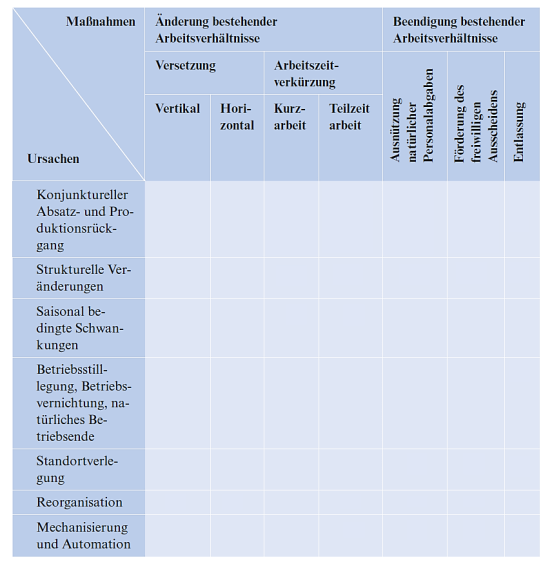
\includegraphics[width=0.55\textwidth]{figures/7_7.png} % Replace with your graphic path
\end{figure}
\solution{
\textbf{a) Maßnahmen bei Personalfreistellung:}
\begin{figure}[H]
    \centering
    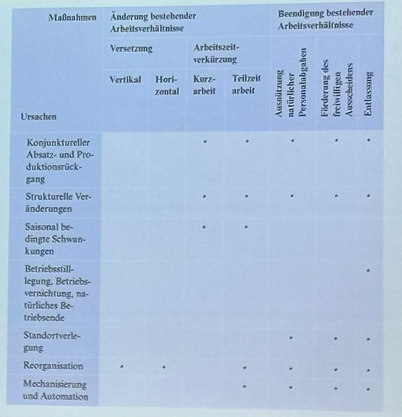
\includegraphics[width=\textwidth]{figures/7_7_2.png}
    \caption{Maßnahmen bei Personalfreistellung}
\end{figure}

\textbf{b) Folgen einer unfreiwilligen Kündigung:}

\textbf{Für die Arbeitnehmer:}
\begin{itemize}
    \item Senkung des Lebensstandards
    \item Verlust der beruflichen Anerkennung
    \item Verlust sozialer Kontakte (Familie, Freundeskreis)
    \item Mögliche Langzeitarbeitslosigkeit
    \item Gesundheitliche Probleme (psychisch oder physisch)
\end{itemize}

\textbf{Für die Arbeitgeber:}
\begin{itemize}
    \item Imageverlust für das Unternehmen
    \item Verschlechterung des Betriebsklimas
    \item Kosten für den Sozialplan
    \item Die genannten negativen Folgen machen die Notwendigkeit eines Outplacement deutlich.
\end{itemize}
}

\exercise{8|1}{Grundlagen der Organisation}

Nennen Sie Gründe und Anlässe, die dazu führen, dass in einem Unternehmen organisiert wird.

\solution{
\textbf{Gründe für die Organisation in Unternehmen:}
\begin{itemize}
    \item Arbeitsteilung
    \item verschiedene Aufgabenarten
    \item hohe Anzahl an Mitarbeitern
\end{itemize}

\textbf{Notwendigkeit zur Organisation:}  
In einem Unternehmen entsteht die Notwendigkeit zur Organisation immer dann, wenn sich die für die formale Organisationsstruktur relevanten Entscheidungsstabstellen und Einflussfaktoren verändert haben.

\textbf{Einflussfaktoren:}  
Diese können in unternehmensinterne und unternehmensexterne Faktoren unterteilt werden:

\begin{itemize}
    \item \textbf{Unternehmensinterne Faktoren, wie z. B.:}
    \begin{itemize}
        \item Wachstum (Eintritt in neue Märkte, Erweiterung des bestehenden Leistungsprogramms, Diversifikation)
        \item Straffung des Leistungsprogramms
        \item Kooperationen
        \item neue EDV-Systeme
        \item neue Technologien
        \item Kosten- und Synergieüberlegungen (z. B. Zusammenlegung von Standorten)
    \end{itemize}
    \item \textbf{Unternehmensexterne Faktoren, wie z. B.:}
    \begin{itemize}
        \item rechtliche Regelungen (z. B. in den Bereichen Arbeits- und Wirtschaftsrecht)
        \item Einfluss der Anspruchsgruppen (z. B. ökologische Aspekte)
        \item wirtschaftliche Lage (z. B. Rezession)
    \end{itemize}
\end{itemize}
}

\exercise{8|2}{Aufbau- und Ablauforganisation}

Jedes Unternehmen steht vor dem Problem, Strukturen und Prozesse festzulegen. Dazu dienen die Aufbau- und Ablauforganisation.

\begin{enumerate}[label=\alph*)]
    \item Zeigen Sie allgemein die Zusammenhänge zwischen der Aufbau- und der Ablauforganisation.
    \item Beschreiben Sie an einem selbst gewählten Beispiel die Zusammenhänge zwischen der Aufbau- und der Ablauforganisation.
\end{enumerate}

\solution{
\begin{enumerate}[label=\alph*)]
    \item \textbf{Allgemeine Zusammenhänge zwischen Aufbau- und Ablauforganisation:}
    \begin{itemize}
        \item Aufbau- und Ablauforganisation hängen sehr eng zusammen.
        \item Beide betrachten das gleiche Objekt, wenn auch unter verschiedenen Aspekten.
        \item Sie bedingen sich gegenseitig und bauen aufeinander auf.
        \item Die Aufbauorganisation liefert den organisatorischen Rahmen, innerhalb dessen die erforderlichen Prozesse der Ablauforganisation vollziehen.
        \item Ausgangspunkt der Ablauforganisation stellen die durch die Aufgabenanalyse gewonnenen Elementaraufgaben dar.
        \item Die Arbeitsanalyse und -synthese als Aspekte der Ablauforganisation bauen auf den Ergebnissen der Aufgabenanalyse auf.
        \item Als erster Schritt steht die Aufgabenanalyse, welche die Gesamtaufgabe in einzelne Elementaraufgaben gliedert.
        \item Darauf aufbauend werden aus einem mithilfe der Aufgabenanalyse gewonnenen Aufgabenkomplex gebildete Einheiten (z. B. Abteilungen oder anderen Aufgabenträgern) zugeordnet (Aufbauorganisation).
        \item Zur Ausführung kommen die in der Arbeitsanalyse auf die Elementaraufgaben zerlegten Aufgaben in Form der Ablauforganisation, d. h. Tätigkeiten zur Erfüllung einer Aufgabe werden unter Berücksichtigung des Arbeitsablaufs, der Arbeitszeit und der Arbeitsmittel zusammengefasst.
    \end{itemize}

    \item \textbf{Beispiel für die Zusammenhänge:}\\
    (Hier kann ein beliebiges Beispiel eingefügt werden, das die Zusammenhänge zwischen Aufbau- und Ablauforganisation verdeutlicht, z. B. die Organisation eines Produktionsprozesses in einem Unternehmen.)
\end{enumerate}
}

\exercise{8|3}{Formale vs. informale Organisation}
In jeder Organisation existieren neben der bewusst gestalteten formalen Organisationsstruktur auch informale Strukturen.

\begin{enumerate}[label=\alph*)]
    \item Wie erkennen Sie formale und informale Organisationsstrukturen? Geben Sie Beispiele für informale Organisationssituationen.
    \item Welche Bedeutung hat die informale Organisation in Bezug auf die Erreichung der Unternehmensziele?
\end{enumerate}

\solution{
\begin{enumerate}[label=\alph*)]
    \item 
    \textbf{Formale Organisationsstruktur:}
    \begin{itemize}
        \item Bei der formalen Struktur handelt es sich um die bewusst gestaltete Organisation.
        \item Hier werden die Abläufe und der Aufbau (Stellenbildung) beschrieben.
    \end{itemize}
    \textbf{Informale Organisationsstruktur:}
    \begin{itemize}
        \item Informale Strukturen bilden sich aus der betrieblichen Wirklichkeit heraus und treten neben oder anstelle der formalen Organisation.
        \item Als Ursache dieser Erscheinung können menschliche Eigenheiten (z. B. Sympathie, gemeinsame Interessen), der soziale Status der Mitglieder des Unternehmens (z. B. Management- vs. Facharbeiterebene), die Arbeitsbedingungen (z. B. Zeitdruck) oder die zu lösende Aufgabe (z. B. ein spezielles Projekt) genannt werden.
        \item Über die informale Organisation gibt es zumeist keine Dokumentation, da sie schwieriger zu erfassen und zu dokumentieren ist als die formale.
        \item Manchmal ist sie auch Ausdruck von Unzufriedenheit der Mitarbeitenden gegenüber der formalen Organisation, respektive von mangelnder Praktikabilität in der betrieblichen Realität.
    \end{itemize}
    
    \item 
    \textbf{Bedeutung der informalen Organisation:}
    \begin{itemize}
        \item Über die Auswirkungen der informalen Struktur kann keine allgemeingültige Aussage gemacht werden.
        \item Eine informale Struktur kann die Kommunikation und somit die Zusammenarbeit der Mitarbeitenden fördern, was sich wiederum positiv auf die Erreichung der Unternehmensziele auswirkt.
        \item Sie kann aber auch negative Auswirkungen in Form von ineffizienten Abläufen haben.
        \item Wichtig ist in jedem Fall, sich der informalen Struktur bewusst zu werden, um positive Wirkungen zu fördern und Konflikte zu beseitigen.
    \end{itemize}
\end{enumerate}
}

\exercise{8|4}{Dilemma der Ablaufplanung}
Erläutern Sie das Dilemma der Ablaufplanung.  
In welchen Unternehmen spielt diese Problematik eine besonders große Rolle?

\solution{
\begin{itemize}
    \item Bei der Ablaufplanung sind folgende Grundsätze einzuhalten:
    \begin{itemize}
        \item Prinzip der Termineinhaltung
        \item Prinzip der Zeitminimierung
        \item Prinzip der Kapazitätsauslastung
    \end{itemize}
    \item Die letzten beiden Grundsätze lassen sich nur selten gleichzeitig verwirklichen.
    \item Gutenberg spricht in diesem Fall vom Dilemma der Ablaufplanung.
    \item Das eigentliche Ziel der Ablauforganisation besteht somit in der optimalen Abstimmung dieser beiden Forderungen.
    \item Es geht darum, die Durchlaufzeit des Materials und die Leerzeiten von Maschinen und Menschen gleichzeitig zu minimieren.
    \item Dieses Dilemma spielt vor allem in großen Unternehmen mit Fließbandproduktion eine große Rolle.
    \item Durch die Digitalisierung gelingt es Unternehmen heute immer besser, mit dem Dilemma der Ablaufplanung umzugehen.
    \item Durch den Einsatz Künstlicher Intelligenz und die digitale Vernetzung der Wertschöpfungsprozesse (z. B. durch Internet of Things) gelingt es, Zeitminimierung und Kapazitätsauslastung optimal aufeinander abzustimmen.
\end{itemize}
}

\exercise{8|5}{Organisationsformen in der Praxis}
Beschreiben Sie, um welche Formen der Aufbauorganisation es sich in den folgenden Fällen jeweils handelt. Begründen Sie Ihre Entscheidung.

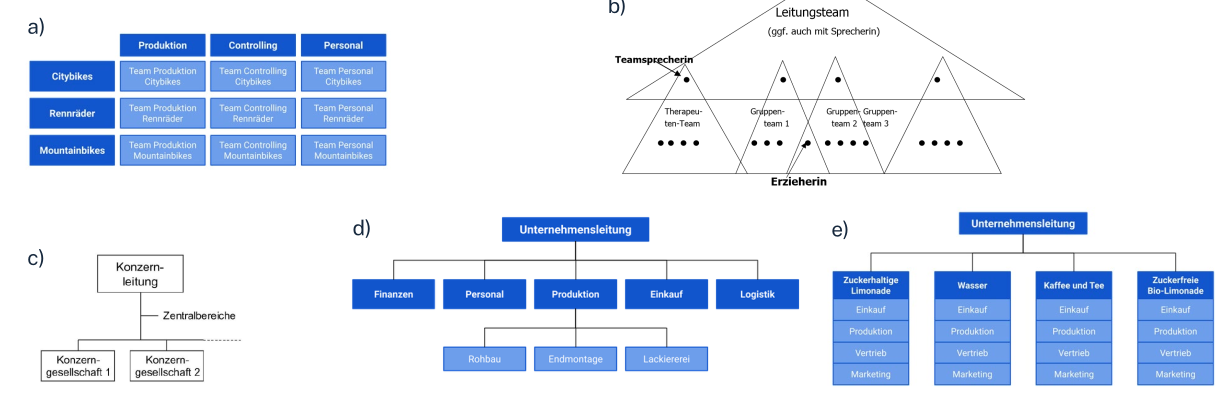
\includegraphics[width=\textwidth]{figures/8_5.png}

\solution{
\begin{itemize}
    \item \textbf{a) Matrixorganisation:} \\
    Beschreibung und Begründung der Entscheidung für die Matrixorganisation.
    \item \textbf{b) Teamorganisation eines Kindergartens:} \\
    Beschreibung und Begründung der Entscheidung für die Teamorganisation.
    \item \textbf{c) Holding:} \\
    Beschreibung und Begründung der Entscheidung für die Holding-Struktur.
    \item \textbf{d) Funktionale Organisation:} \\
    Beschreibung und Begründung der Entscheidung für die Funktionale Organisation.
    \item \textbf{e) Spartenorganisation:} \\
    Beschreibung und Begründung der Entscheidung für die Spartenorganisation.
\end{itemize}
}


\exercise{9\textbar 1}{Entscheidung bei Handlungsalternativen}
Ein Unternehmen muss sich zwischen den beiden folgenden Handlungsalternativen entscheiden:

\begin{itemize}
    \item \textbf{A:} Beibehaltung des bisherigen Sortiments
    \item \textbf{B:} Ergänzung des bisherigen Sortiments durch ein neues Produkt
\end{itemize}

Alternative A bringt mit absoluter Sicherheit einen Gewinn von 50 €.
Der Erfolg der Alternative B dagegen ist ungewiss. Mit einer Eintrittswahrscheinlichkeit von $g = 0,20$ wird ein Gewinn in Höhe von 2.000 € erwartet. Mit größerer Wahrscheinlichkeit ($v = 0,80$) muss dagegen mit einem Verlust in Höhe von 400 € gerechnet werden.

\begin{enumerate}[label=(\alph*)]
    \item Wie groß ist der mathematische Erwartungswert des Erfolges aus Handlungsalternative B?
    \item Soll sich der Betrieb für Alternative A oder B entscheiden? Begründen Sie Ihre Antwort.
\end{enumerate}

\solution{

\begin{enumerate}[label=(\alph*)]
    \item \textbf{Mathematischer Erwartungswert für Alternative B:}

    Der mathematische Erwartungswert $E(B)$ wird berechnet, indem die möglichen Gewinne und Verluste mit ihren jeweiligen Wahrscheinlichkeiten gewichtet und anschließend summiert werden:

    \[
    E(B) = g \cdot \text{Gewinn} + v \cdot \text{Verlust}
    \]

    Einsetzen der Werte:

    \[
    E(B) = 0,20 \cdot 2.000 + 0,80 \cdot (-400)
    \]

    Berechnung:

    \[
    E(B) = 400 - 320 = 80
    \]

    Der mathematische Erwartungswert für Alternative B beträgt 80 €.

    \item \textbf{Entscheidung zwischen Alternative A und B:}

    Alternative A bietet einen sicheren Gewinn von 50 €.
    Alternative B hat einen mathematischen Erwartungswert von 80 €, jedoch ist der Erfolg unsicher, da auch ein Verlust von 400 € möglich ist.

    \textbf{Empfehlung:} Der Betrieb sollte sich für Alternative B entscheiden, da der mathematische Erwartungswert höher ist als der sichere Gewinn aus Alternative A. Allerdings hängt die Entscheidung auch von der Risikobereitschaft des Unternehmens ab. Ein risikoscheues Unternehmen könnte aufgrund der Unsicherheit Alternative A bevorzugen.
\end{enumerate}
}

\exercise{9\textbar 2}{Entscheidungsregeln (A1)}
Die verantwortlichen Stellen eines Unternehmens stehen oft vor dem Problem, dass sie Entscheidungen treffen müssen, ohne über die dazu notwendige Sicherheit in Bezug auf deren Auswirkungen zu verfügen.\\
Für solche Situationen sind Regeln entwickelt worden, die eine Entscheidung erleichtern sollen.

\begin{enumerate}[label=(\alph*)]
    \item Erklären Sie mit dem obenstehenden Beispiel die folgenden Entscheidungsregeln:
    \begin{itemize}
        \item Maximierung des Gesamterwartungswertes
        \item Minimax-Regel
        \item Maximax-Regel
        \item Pessimismus-Optimismus-Regel
        \item Minimax-Risiko-Regel
    \end{itemize}
    \item Welche Einwände können gegen die Entscheidungsregeln vorgebracht werden?
\end{enumerate}
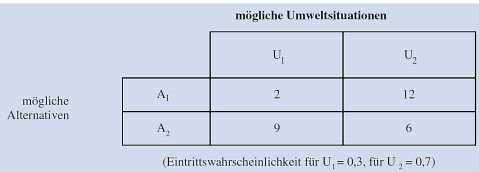
\includegraphics[width=0.6\textwidth]{figures/9_2.png}

\exercise{9\textbar 3}{Entscheidungsregeln (A2)}
Herr Unschlüssig will ein neues Produkt herstellen. Zur Wahl stehen drei Produkte, wobei Herr Unschlüssig sowohl den minimalen als auch den maximalen Gewinn kennt, der aus dem Verkauf dieser Produkte resultieren könnte.

\begin{table}[h!]
\centering
\begin{tabular}{|c|c|c|}
\hline
\textbf{Produkt} & \textbf{Minimaler Gewinn} & \textbf{Maximaler Gewinn} \\
\hline
Produkt 1 & 390 & 430 \\
\hline
Produkt 2 & 410 & 410 \\
\hline
Produkt 3 & 400 & 420 \\
\hline
\end{tabular}
\caption{Mögliche Gewinne der Produkte}
\end{table}

\begin{enumerate}[label=(\alph*)]
    \item Treffen Sie die optimale Wahl mithilfe des Hurwicz-Kriteriums (Pessimismus-Optimismus-Kriterium), wenn der Pessimismus-Optimismus-Faktor \( \alpha = 0{,}2 \) beträgt.
    \item Bestimmen Sie den kritischen Wert des Pessimismus-Optimismus-Faktors, bei dem die Alternativen „Produkt 1“ und „Produkt 2“ gerade gleichwertig sind.
    \item Beurteilen Sie dieses Verfahren.
\end{enumerate}

\solution{

\begin{enumerate}[label=(\alph*)]
    \item \textbf{Berechnung der optimalen Wahl mit dem Hurwicz-Kriterium:}

    Für das Hurwicz-Kriterium wird die Formel \( H = \alpha \cdot \text{minimaler Gewinn} + (1 - \alpha) \cdot \text{maximaler Gewinn} \) verwendet.
    
    \begin{align*}
        H_{\text{Produkt 1}} &= 0{,}8 \cdot 390 + 0{,}2 \cdot 430 = 398 \\
        H_{\text{Produkt 2}} &= 0{,}8 \cdot 410 + 0{,}2 \cdot 410 = 410 \\
        H_{\text{Produkt 3}} &= 0{,}8 \cdot 400 + 0{,}2 \cdot 420 = 404
    \end{align*}
    
    \textbf{Ergebnis:} Produkt 2 ist die optimale Wahl.

    \item \textbf{Bestimmung des kritischen Wertes von \( \alpha \):}

    Zwei Alternativen sind gleichwertig, wenn ihre Hurwicz-Werte identisch sind. Für „Produkt 1“ und „Produkt 2“ gilt:
    
    \[
    390 \cdot \alpha + 430 \cdot (1 - \alpha) = 410 \cdot \alpha + 410 \cdot (1 - \alpha)
    \]
    
    Auflösen ergibt:
    \[
    \alpha = 0{,}5
    \]

    \item \textbf{Beurteilung des Verfahrens:}
    \begin{itemize}
        \item Problem der unsicheren Informationen (Erfassung, Gewichtung) 
        \item keine Berücksichtigung der individuellen Lage des Unternehmens
        \item Risikofaktoren nur schwer einzuschätzen (nicht quantifizierbar)
        \item Keine Berücksichtigung irrationaler Faktoren
        \item Besstimmung des Pessimisum-Optimismus-Faktors ist sehr subjektiv
    \end{itemize}
\end{enumerate}
}

\exercise{9\textbar 4}{Entscheidungsregeln (A3)}
Die Möbel AG steht vor der schwierigen Entscheidung, wie sie ihr Sortiment in Zukunft gestalten soll. Drei Strategien sind möglich:

\begin{itemize}
    \item Produktion und Vertrieb von nachgebauten antiken Möbeln erster Qualität.
    \item Produktion und Vertrieb von modernen Designermöbeln der obersten Preisklasse.
    \item Produktion und Vertrieb von klassischen Möbeln mit mittlerem Preisniveau.
\end{itemize}

Die Entwicklung des Absatzes für den Möbelmarkt wird von den Marktforschungsexperten wie folgt beurteilt:
\begin{enumerate}
    \item Stetiges Wachstum des Bedarfs an Möbeln, gleiche Anbieterstruktur.
    \item Absatz wird sich wegen einer wirtschaftlichen Stagnation verringern.
    \item Stetiges Wachstum, aber verschärfte Konkurrenz unter den Anbietern.
\end{enumerate}

Die durchschnittlichen Jahresgewinne in Abhängigkeit der verschiedenen zukünftigen Marktsituationen werden wie in der unten stehenden Tabelle geschätzt (Gewinne in 1.000 €).

\begin{table}[h!]
    \centering
    \begin{tabular}{|l|c|c|c|}
        \hline
        \textbf{Strategie} & \textbf{Marktsituation 1} & \textbf{Marktsituation 2} & \textbf{Marktsituation 3} \\
        \hline
        Antike Möbel & 85 & 35 & 58 \\
        \hline
        Designermöbel & 94 & 45 & 86 \\
        \hline
        Klassische Möbel & 76 & 58 & 68 \\
        \hline
    \end{tabular}
    \caption{Gewinne je nach Marktsituation (in 1.000 €)}
    \label{tab:moebel_gewinn}
\end{table}

\begin{enumerate}[label=(\alph*)]
    \item Welche Strategie würde nach dem Minimax-Prinzip gewählt werden?
    \item Welche Strategie wählen Sie mithilfe des Maximax-Prinzips?
    \item Beurteilen Sie die beiden Verfahren.
\end{enumerate}

\solution{

\begin{enumerate}[label=(\alph*)]
    \item \textbf{Minimax-Prinzip:}
    \begin{itemize}
        \item Schritt 1: Minimalen Gewinn pro Strategie bestimmen:
        \begin{itemize}
            \item Antike Möbel: 35
            \item Designermöbel: 45
            \item Klassische Möbel: 58
        \end{itemize}
        \item Schritt 2: Variante mit dem höchsten minimalen Gewinn auswählen. Es wird die Strategie \textbf{Klassische Möbel} ausgewählt.
    \end{itemize}

    \item \textbf{Maximax-Prinzip:}
    \begin{itemize}
        \item Schritt 1: Maximalen Gewinn pro Strategie bestimmen:
        \begin{itemize}
            \item Antike Möbel: 85
            \item Designermöbel: 94
            \item Klassische Möbel: 76
        \end{itemize}
        \item Schritt 2: Variante mit dem höchsten maximalen Gewinn auswählen. Es wird die Strategie \textbf{Designermöbel} ausgewählt.
    \end{itemize}

    \item \textbf{Beurteilung der Verfahren:}
    \begin{itemize}
        \item \textbf{Allgemeine Nachteile der Entscheidungsregeln:}
        \begin{itemize}
            \item Problem der unsicheren Informationen (Erfassung, Gewichtung).
            \item Keine Berücksichtigung der individuellen Lage des Unternehmens.
            \item Risikofaktoren nur schwer einzuschätzen (nicht quantifizierbar).
            \item Keine Berücksichtigung irrationaler Faktoren.
        \end{itemize}

        \item \textbf{Spezielle Nachteile der Entscheidungsregeln:}
        \begin{itemize}
            \item \textbf{Minimax-Regel:}
            \begin{itemize}
                \item Das Risiko der Entscheidungssituation wird nicht berücksichtigt, da die verschiedenen Umweltsituationen nicht gewichtet werden.
                \item Es kann zwar das schlechteste mögliche Ergebnis eintreten, jedoch wird selten das bestmögliche Ergebnis erreicht.
            \end{itemize}
            \item \textbf{Maximax-Regel:}
            \begin{itemize}
                \item Das Risiko der Entscheidungssituation wird ebenfalls nicht berücksichtigt.
                \item Es kann zwar die Alternative mit dem bestmöglichen Ergebnis erreicht werden, jedoch meistens nur unter hohem Risiko.
            \end{itemize}
        \end{itemize}
    \end{itemize}
\end{enumerate}
}
\exercise{9\textbar 5}{Produkt-Markt-Strategien}
Beschreiben Sie am Beispiel eines Herstellers von Gummib\"archen die vier Produkt-Markt-Strategien.

\solution{

\begin{enumerate}
    \item \textbf{Marktdurchdringung:} Der Hersteller k\"onnte seine bestehenden Gummib\"archen intensiver vermarkten, z.\,B. durch Rabattaktionen oder Werbung, um die Verkaufszahlen zu steigern.
    
    \item \textbf{Marktentwicklung:} Das Unternehmen k\"onnte neue M\"arkte erschlie\"sen, indem es Gummib\"archen in L\"ander exportiert, in denen sie bisher noch nicht angeboten wurden.
    
    \item \textbf{Produktentwicklung:} Der Hersteller k\"onnte neue Varianten der Gummib\"archen entwickeln, z.\,B. mit exotischen Geschmacksrichtungen oder in Form von zuckerfreien Produkten.
    
    \item \textbf{Diversifikation:} Das Unternehmen k\"onnte komplett neue Produkte einf\"uhren, die nichts mit Gummib\"archen zu tun haben, z.\,B. Schokolade oder Snacks.
\end{enumerate}
}
\exercise{9\textbar 6}{Produkt-Markt-Strategien vs. Wettbewerbsstrategien}
Wodurch unterscheiden sich Produkt-Markt-Strategien von Wettbewerbsstrategien?

\solution{

\begin{itemize}
    \item \textbf{Produkt-Markt-Strategien:}
    \begin{itemize}
        \item Produkt-Markt-Strategien konzentrieren sich darauf, wie ein Unternehmen neue oder bestehende Produkte in bestehenden oder neuen Märkten positionieren kann.
        \item Die vier zentralen Ansätze sind:
        \begin{itemize}
            \item \textbf{Marktdurchdringung:} Steigerung des Absatzes bestehender Produkte in bestehenden Märkten.
            \item \textbf{Marktentwicklung:} Einführung bestehender Produkte in neue Märkte.
            \item \textbf{Produktentwicklung:} Entwicklung neuer Produkte für bestehende Märkte.
            \item \textbf{Diversifikation:} Einführung neuer Produkte in neue Märkte.
        \end{itemize}
    \end{itemize}

    \item \textbf{Wettbewerbsstrategien:}
    \begin{itemize}
        \item Wettbewerbsstrategien legen den Schwerpunkt darauf, wie ein Unternehmen sich gegenüber seinen Mitbewerbern in einem Markt differenzieren und positionieren kann.
        \item Die drei grundlegenden Strategien nach Porter sind:
        \begin{itemize}
            \item \textbf{Kostenführerschaft:} Minimierung der Kosten, um Produkte zu einem niedrigeren Preis als die Konkurrenz anbieten zu können.
            \item \textbf{Differenzierung:} Schaffung eines einzigartigen Wertes für Kunden, beispielsweise durch Qualität, Marke oder Service.
            \item \textbf{Fokussierung:} Konzentration auf eine spezielle Nische, entweder durch Kostenführerschaft oder Differenzierung in einem begrenzten Marktsegment.
        \end{itemize}
    \end{itemize}

    \item \textbf{Unterschiede:}
    \begin{itemize}
        \item Produkt-Markt-Strategien zielen darauf ab, Wachstumschancen zu identifizieren und Produkte und Märkte strategisch auszurichten.
        \item Wettbewerbsstrategien richten den Fokus auf die Positionierung gegenüber Wettbewerbern und die Schaffung von Wettbewerbsvorteilen.
        \item Während Produkt-Markt-Strategien primär auf die Kombination von Märkten und Produkten abzielen, betrachten Wettbewerbsstrategien die Methoden, um in diesen Märkten erfolgreich zu agieren.
    \end{itemize}
\end{itemize}
}
\exercise{9\textbar 7}{Strategische Erfolgspositionen}
Um langfristig überleben zu können, muss ein Unternehmen strategische Erfolgspositionen aufbauen.

\begin{enumerate}[label=(\alph*)]
    \item Was versteht man unter einer strategischen Erfolgsposition?
    \item Welche Bedingungen müssen erfüllt sein, damit man von einer strategischen Erfolgsposition sprechen kann?
    \item Geben Sie Beispiele für strategische Erfolgspositionen Ihnen bekannter Unternehmen.
\end{enumerate}

\solution{
\textbf{Lösung:}

\begin{enumerate}[label=(\alph*)]
    \item \textbf{Definition einer strategischen Erfolgsposition:}
    \begin{itemize}
        \item Eine strategische Erfolgsposition (SEP) beschreibt einen einzigartigen und langfristigen Wettbewerbsvorteil, den ein Unternehmen gegenüber seinen Mitbewerbern besitzt.
        \item Dieser Vorteil ermöglicht es dem Unternehmen, nachhaltig höhere Gewinne zu erzielen, indem es seine Marktposition sichert und ausbaut.
        \item SEPs basieren häufig auf schwer imitierbaren Ressourcen, Fähigkeiten oder Technologien.
    \end{itemize}

    \item \textbf{Bedingungen für eine strategische Erfolgsposition:}
    \begin{itemize}
        \item \textbf{Einzigartigkeit:} Die Position muss sich signifikant von der Konkurrenz unterscheiden.
        \item \textbf{Nachhaltigkeit:} Der Vorteil muss langfristig bestehen und schwer kopierbar sein.
        \item \textbf{Relevanz für den Kunden:} Der Vorteil muss für Kunden einen erkennbaren Mehrwert bieten.
        \item \textbf{Wirtschaftliche Rentabilität:} Die Position muss zu einem Wettbewerbsvorteil führen, der sich in höheren Gewinnen widerspiegelt.
    \end{itemize}

    \item \textbf{Beispiele für strategische Erfolgspositionen:}
    \begin{itemize}
        \item \textbf{Apple:} 
        \begin{itemize}
            \item Starkes Markenimage und hohe Kundenbindung.
            \item Innovationsführerschaft in Design und Technologie (z. B. iPhone, MacBook).
        \end{itemize}
        \item \textbf{Tesla:}
        \begin{itemize}
            \item Führende Position in der Elektromobilität.
            \item Überlegenes Batterie- und Ladesystem sowie eine starke Marke.
        \end{itemize}
        \item \textbf{Coca-Cola:}
        \begin{itemize}
            \item Weltweite Bekanntheit und Markentreue.
            \item Starkes Vertriebsnetzwerk und kontinuierliche Innovationen im Marketing.
        \end{itemize}
        \item \textbf{IKEA:}
        \begin{itemize}
            \item Effiziente Wertschöpfungskette mit Fokus auf Selbstmontage.
            \item Kombination aus niedrigen Preisen und ansprechendem skandinavischen Design.
        \end{itemize}
    \end{itemize}
\end{enumerate}
}

\exercise{9\textbar 8}{Lernkurve vs. Erfahrungskurve}
Sowohl die Lern- als auch die Erfahrungskurve ermöglichen Kostensenkungen im Betrieb.

\begin{enumerate}[label=(\alph*)]
    \item Welches ist der Unterschied zwischen der Lern- und der Erfahrungskurve?
    \item Welchen Zusammenhang sehen Sie zwischen der Erfahrungskurve und den Economies of Scale?
\end{enumerate}

\solution{

\begin{enumerate}[label=(\alph*)]
    \item \textbf{Unterschied zwischen Lern- und Erfahrungskurve:}
    \begin{itemize}
        \item \textbf{Lernkurve:}
        \begin{itemize}
            \item Beschreibt die Kostensenkung, die durch die Steigerung individueller Fähigkeiten und Effizienz bei der Wiederholung einer Tätigkeit erreicht wird.
            \item Fokus liegt auf der Produktivität der Mitarbeiter und der kontinuierlichen Verbesserung der Arbeitsabläufe.
            \item Beispiel: Ein Mitarbeiter benötigt für die Montage eines Produkts weniger Zeit, je häufiger er die Aufgabe wiederholt.
        \end{itemize}
        \item \textbf{Erfahrungskurve:}
        \begin{itemize}
            \item Betrachtet die gesamte Wertschöpfungskette und berücksichtigt Skaleneffekte, Technologieverbesserungen und organisatorisches Lernen.
            \item Besagt, dass mit jeder Verdopplung der kumulierten Produktionsmenge die Stückkosten um einen konstanten Prozentsatz sinken.
            \item Umfasst mehr Faktoren als die Lernkurve, wie zum Beispiel Automatisierung, bessere Ressourcennutzung und Innovationsprozesse.
        \end{itemize}
        \item \textbf{Zusammenfassung des Unterschieds:}
        \begin{itemize}
            \item Die Lernkurve fokussiert sich auf individuelle und arbeitsbezogene Verbesserungen.
            \item Die Erfahrungskurve bezieht sich auf unternehmensweite Effizienzsteigerungen entlang der gesamten Wertschöpfungskette.
        \end{itemize}
    \end{itemize}

    \item \textbf{Zusammenhang zwischen Erfahrungskurve und Economies of Scale:}
    \begin{itemize}
        \item Die Erfahrungskurve und die Economies of Scale sind eng miteinander verbunden, da beide Mechanismen auf Kostensenkungen durch Produktionssteigerungen abzielen.
        \item \textbf{Economies of Scale:}
        \begin{itemize}
            \item Kostenvorteile, die durch die Steigerung des Produktionsvolumens erreicht werden.
            \item Fixkosten werden auf eine größere Menge an Produkten verteilt, was die Stückkosten senkt.
        \end{itemize}
        \item \textbf{Erfahrungskurve:}
        \begin{itemize}
            \item Geht über die Economies of Scale hinaus, da sie auch Lern- und Effizienzsteigerungen durch technologische Innovationen und organisatorisches Wissen berücksichtigt.
        \end{itemize}
        \item \textbf{Zusammenhang:}
        \begin{itemize}
            \item Beide Konzepte wirken oft gemeinsam: Höhere Produktionsmengen führen zu Skaleneffekten (Economies of Scale) und fördern gleichzeitig das Sammeln von Erfahrungen, die zusätzliche Kostensenkungen ermöglichen.
            \item Beispiel: In der Automobilproduktion können große Stückzahlen (Economies of Scale) die Fixkosten senken, während gleichzeitig Prozessinnovationen (Erfahrungskurve) die variablen Kosten reduzieren.
        \end{itemize}
    \end{itemize}
\end{enumerate}
}

\exercise{9\textbar 9}{Wettbewerbsstrategien}
Wettbewerbsstrategien sollen es dem Unternehmen ermöglichen, sich gegenüber der Konkurrenz im Markt zu behaupten, indem sie einen erfolgreichen Umgang mit den Wettbewerbskräften erlauben.

\begin{enumerate}[label=(\alph*)]
    \item Welche Wettbewerbsstrategien unterscheidet Porter?
    \item Zeigen Sie, welche Gefahren und Risiken mit den verschiedenen Wettbewerbsstrategien verbunden sind.
\end{enumerate}

\solution{
\textbf{Lösung:}

\begin{enumerate}[label=(\alph*)]
    \item \textbf{Wettbewerbsstrategien nach Porter:}
    Michael E. Porter unterscheidet in seinem Modell drei generische Wettbewerbsstrategien, die Unternehmen nutzen können, um Wettbewerbsvorteile zu erzielen:
    \begin{itemize}
        \item \textbf{Kostenführerschaft:}
        \begin{itemize}
            \item Ziel ist es, durch geringe Kosten und eine effiziente Produktion die niedrigsten Preise im Markt anzubieten.
            \item Beispiele: Einsatz von Skaleneffekten, Standardisierung, Automatisierung.
        \end{itemize}
        \item \textbf{Differenzierung:}
        \begin{itemize}
            \item Ziel ist es, sich durch einzigartige Produkte oder Dienstleistungen von der Konkurrenz abzuheben.
            \item Beispiele: Markenbildung, Produktinnovationen, hoher Kundenservice.
        \end{itemize}
        \item \textbf{Fokussierung:}
        \begin{itemize}
            \item Konzentration auf eine bestimmte Nische oder ein Marktsegment.
            \item Ziel ist es, in diesem Bereich entweder Kostenführerschaft oder Differenzierung zu erreichen.
        \end{itemize}
    \end{itemize}

    \item \textbf{Gefahren und Risiken der Wettbewerbsstrategien:}
    \begin{itemize}
        \item \textbf{Kostenführerschaft:}
        \begin{itemize}
            \item \textbf{Gefahr der Preiskriege:} Wettbewerber können ebenfalls die Preise senken, wodurch die Margen stark schrumpfen.
            \item \textbf{Qualitätsprobleme:} Starke Kostenreduktionen können zu einer Verschlechterung der Produkt- oder Servicequalität führen.
            \item \textbf{Abhängigkeit von Skaleneffekten:} Ein Rückgang der Nachfrage kann die Kostenvorteile gefährden.
        \end{itemize}
        \item \textbf{Differenzierung:}
        \begin{itemize}
            \item \textbf{Hohe Kosten:} Differenzierung erfordert oft erhebliche Investitionen in Forschung, Entwicklung und Marketing.
            \item \textbf{Nachahmung durch Wettbewerber:} Einzigartige Merkmale können kopiert werden, wodurch der Differenzierungsvorteil verloren geht.
            \item \textbf{Marktveränderungen:} Kundenpräferenzen können sich ändern, wodurch die Differenzierungsstrategie unwirksam wird.
        \end{itemize}
        \item \textbf{Fokussierung:}
        \begin{itemize}
            \item \textbf{Begrenztes Marktpotenzial:} Die Zielgruppe ist oft klein, was das Wachstum einschränkt.
            \item \textbf{Abhängigkeit von der Nische:} Veränderungen in der Nische können existenzbedrohend sein.
            \item \textbf{Angriffe durch größere Unternehmen:} Große Anbieter können die Nische ebenfalls bedienen und kleinere Wettbewerber verdrängen.
        \end{itemize}
    \end{itemize}
\end{enumerate}
}

\exercise{9\textbar 10}{Wettbewerbskräfte, Wettbewerbsstrategie und Preisstrategie}
Die Panorama AG ist im Pharmabereich tätig. 40~\% des Umsatzes werden mit Erkältungsmitteln, weitere 35~\% mit Schlafmitteln und die restlichen 25~\% mit Aufbaupräparaten erzielt.

Mit 250 Mitarbeitenden wird ein Jahresumsatz von 32 Mio. € erzielt, der zu fast 100~\% in Deutschland erarbeitet wird. Der Cashflow beträgt 4,2 Mio. €.

Das Unternehmen beabsichtigt, ein von ihm selbst entwickeltes Medikament zu lancieren. Das neue Produkt dient der Vorbeugung gegen Erkältungskrankheiten und kann das ganze Jahr hindurch eingenommen werden.

Marktuntersuchungen haben ergeben, dass zwei bis drei Jahre nach der Lancierung mit einem Marktanteil von 5~\% gerechnet werden kann. Es ist nicht damit zu rechnen, dass der Marktanteil in ferner Zukunft wesentlich vergrößert werden kann.

\begin{enumerate}[label=(\alph*)]
    \item Welchen Wettbewerbskräften sieht sich das Unternehmen bei der Markteinführung seines neuen Produktes gegenüber?
    \item Welche Wettbewerbsstrategie für das neue Produkt würden Sie dem Unternehmen empfehlen?
    \item Auf welche Erhebungstechnik könnte die Panorama AG ihre Marktforschung gestützt haben?
    \item Nach welchen Kriterien wird die Preisstrategie für das neue Medikament zu wählen sein?
\end{enumerate}

\solution{
\textbf{Lösung:}

\begin{enumerate}[label=(\alph*)]
    \item \textbf{Wettbewerbskräfte nach Porter:}
    Die Panorama AG sieht sich bei der Markteinführung des neuen Produkts den folgenden Wettbewerbskräften gegenüber:
    \begin{itemize}
        \item Verhandlungsmacht der Abnehmer.
        \item Verhandlungsmacht der Lieferanten.
        \item Bedrohung durch Ersatzprodukte und -dienste.
        \item Bedrohung durch neue Konkurrenten.
        \item Rivalität unter den bestehenden Unternehmen.
    \end{itemize}

    \item \textbf{Empfohlene Wettbewerbsstrategie:}
    \begin{itemize}
        \item Die Panorama AG betreibt bereits eine Nischenstrategie in Bezug auf ihre bisherigen Produkte.
        \item Da mit dem neuen Produkt nur ein Marktanteil von 5~\% zu rechnen ist und das Unternehmen bereits im Marktsegment „Erkältungsmittel“ tätig ist, bietet sich eine \textbf{Nischenstrategie} für das neue Produkt in diesem Segment an.
        \item Gleichzeitig könnte eine \textbf{Differenzierungsstrategie} verfolgt werden, da die geringe Größe des Marktanteils wenig Raum für Economies of Scale lässt und damit die Kostenführerschaft erschwert wird.
        \item Zusätzliche Faktoren wie kartellähnliche Strukturen in der Medikamentenbranche könnten die Wahl einer Kostenführerschaft-Strategie zusätzlich einschränken.
    \end{itemize}

    \item \textbf{Erhebungsmethoden:}
    Die Panorama AG könnte ihre Marktforschung auf folgende Erhebungsansätze gestützt haben:
    \begin{itemize}
        \item \textbf{Primärforschung:}
        \begin{itemize}
            \item Befragungen von Endverbrauchern, um die Akzeptanz des neuen Medikaments zu ermitteln.
            \item Interviews mit Fachleuten, z. B. Ärzten oder Apothekern, die die Verschreibung und Empfehlung beeinflussen.
        \end{itemize}
        \item \textbf{Sekundärforschung:}
        \begin{itemize}
            \item Analyse von bestehenden Marktstudien und Daten zur Nachfrage nach Erkältungsmedikamenten.
            \item Untersuchung von Wettbewerbsprodukten und deren Marktposition.
        \end{itemize}
    \end{itemize}

    \item \textbf{Kriterien zur Preisstrategie:}
    Die Preisstrategie für das neue Medikament sollte auf den folgenden Kriterien basieren:
    \begin{itemize}
        \item \textbf{Kostenbasierte Preisgestaltung:}
        \begin{itemize}
            \item Berücksichtigung der Produktionskosten sowie Forschung und Entwicklung.
        \end{itemize}
        \item \textbf{Wettbewerbsorientierte Preisgestaltung:}
        \begin{itemize}
            \item Analyse der Preise vergleichbarer Produkte auf dem Markt.
            \item Positionierung des Preises, um sich von Konkurrenzprodukten abzuheben.
        \end{itemize}
        \item \textbf{Wertorientierte Preisgestaltung:}
        \begin{itemize}
            \item Wahrnehmung des Kundennutzens, z. B. Prävention von Erkältungskrankheiten und einfache Anwendung.
        \end{itemize}
    \end{itemize}
\end{enumerate}
}

\exercise{9\textbar 11}{Kurzfristige Planung bei unsicherer Wirtschaftslage}
Nehmen Sie zur folgenden Aussage Stellung:
\begin{quote}
    „Je unsicherer die Wirtschaftslage ist, umso kurzfristiger muss die Planung sein.“
\end{quote}

\solution{

Die Aussage, „Je unsicherer die Wirtschaftslage ist, umso kurzfristiger muss die Planung sein“, lässt sich wie folgt bewerten:

\begin{itemize}
    \item \textbf{Begründung für kurzfristige Planung:}
    \begin{itemize}
        \item \textbf{Flexibilität:} Unsichere Wirtschaftslagen erfordern schnelle Reaktionen auf Änderungen in den Marktbedingungen, wie z. B. Schwankungen der Nachfrage oder Rohstoffpreise.
        \item \textbf{Risikominimierung:} Längerfristige Planungen bergen ein höheres Risiko von Fehlentscheidungen, da unvorhergesehene Ereignisse (z. B. Krisen oder wirtschaftliche Einbrüche) die Planungsgrundlage verändern können.
        \item \textbf{Kostenkontrolle:} Kurzfristige Planung ermöglicht es, Budgets und Investitionen besser an aktuelle Gegebenheiten anzupassen und so unnötige Kosten zu vermeiden.
    \end{itemize}

    \item \textbf{Gegenargumente:}
    \begin{itemize}
        \item \textbf{Langfristige Perspektive:} Auch in unsicheren Zeiten ist eine langfristige Planung wichtig, um strategische Ziele nicht aus den Augen zu verlieren. Dies betrifft insbesondere Investitionen in Forschung und Entwicklung oder den Aufbau neuer Märkte.
        \item \textbf{Planungsunsicherheit:} Kurzfristige Planungen können dazu führen, dass Entscheidungen zu oft geändert werden müssen, was wiederum zu Instabilität und Ineffizienz führt.
    \end{itemize}

    \item \textbf{Kombination aus kurz- und langfristiger Planung:}
    \begin{itemize}
        \item \textbf{Szenarioplanung:} Unsichere Wirtschaftslagen können mit einer Kombination aus kurz- und langfristigen Plänen bewältigt werden, indem alternative Szenarien berücksichtigt werden.
        \item \textbf{Rollierende Planung:} Ein Ansatz, der regelmäßige Anpassungen der langfristigen Planung vorsieht, kann Unsicherheiten besser abfedern.
    \end{itemize}

    \item \textbf{Fazit:}
    Die Aussage ist nicht uneingeschränkt gültig. Während eine kurzfristige Planung in unsicheren Wirtschaftslagen Vorteile bietet, bleibt eine langfristige Perspektive für die Sicherung der Wettbewerbsfähigkeit und strategischen Ausrichtung des Unternehmens essenziell. Eine ausgewogene Kombination aus beiden Ansätzen ist der effektivste Weg, um Unsicherheiten zu begegnen.
\end{itemize}
}


\section{VWL}
\exercise{1\textbar 1}{Open-Book-Prinzip}
In manchen Klausuren wird nach dem Prinzip des „Open Book“ vorgegangen, d. h. die Studierenden können ihre Lehrbücher mit in die Klausur nehmen. 

Student Hubert findet, das ist eine tolle Sache. Er kann es überhaupt nicht verstehen, dass seine Kommilitonin Sarah es lieber hätte, wenn die Bücher zu Hause gelassen werden müssten.

\begin{quote}
    Wer hat Recht?
\end{quote}

\solution{

Beide Ansichten spiegeln unterschiedliche Herangehensweisen an die Prüfungsstrategie wider, aber das zugrunde liegende Problem könnte das sogenannte **Konkurrenz-Paradoxon** sein:
\begin{itemize}
    \item \textbf{Pro Open-Book (Hubert):}
    \begin{itemize}
        \item Hubert freut sich über den Zugang zu Lehrbüchern, da sie ihm die Möglichkeit geben, schwierige Details nachzuschlagen und seine Konzentration auf das Verständnis und die Anwendung zu legen.
        \item Das Open-Book-Prinzip kann Prüfungsstress reduzieren, indem Studierende nicht alles auswendig lernen müssen.
    \end{itemize}
    
    \item \textbf{Kontra Open-Book (Sarah):}
    \begin{itemize}
        \item Sarah könnte befürchten, dass durch das Open-Book-Prinzip alle Studierenden die gleiche "Hilfestellung" haben, wodurch das individuelle Verständnis weniger ins Gewicht fällt.
        \item Das Paradoxon besteht darin, dass alle Studierenden theoretisch Zugang zu den gleichen Ressourcen haben. Der Wettbewerbsvorteil verschwindet, und es kommt stärker darauf an, wer besser mit den Ressourcen umgehen kann.
    \end{itemize}
\end{itemize}

\textbf{Fazit:} 
Das Open-Book-Prinzip kann helfen, den Fokus auf Verständnis und Problemlösungsfähigkeiten zu legen. Es stellt jedoch andere Anforderungen an die Studierenden, wie z. B. die Fähigkeit, effizient relevante Informationen zu finden. Es bleibt ein Balanceakt zwischen Chancengleichheit und der Fähigkeit, aus gleichen Ressourcen Vorteile zu ziehen.
}

\exercise{1\textbar 2}{Mikro- und Makroökonomie}
Mikro- und Makroökonomie sind die beiden zentralen Teilgebiete der Volkswirtschaftslehre.

Ordnen Sie die folgenden Fragestellungen in das entsprechende Teilgebiet ein:
\begin{enumerate}
    \item Ist das Zinsniveau in Euroland derzeit zu hoch?
    \item Sollte die Deutsche Post wieder vom Staat betrieben werden?
    \item Soll sich die Bundesregierung bemühen, weiterhin einen ausgeglichenen Haushalt vorzulegen?
    \item Ist es richtig, dass die Europäische Union die Landwirtschaft subventioniert?
    \item Sollte die Leiharbeit in Deutschland ausgeweitet werden?
    \item Sollte für Studentenwohnungen ein Höchstpreis eingeführt werden?
    \item Welche Auswirkungen hat ein Kurseinbruch an den Aktienmärkten?
    \item Soll die Ökosteuer noch weiter erhöht werden?
    \item Kommt es im nächsten Jahr zu einem kräftigen Wirtschaftswachstum in Deutschland?
    \item Soll der Zahnersatz von den Gesetzlichen Krankenkassen vollständig bezahlt werden?
\end{enumerate}

\solution{

\begin{itemize}
    \item \textbf{Mikroökonomie:} Untersuchung einzelner Märkte, Entscheidungen einzelner Akteure und deren Einfluss auf Angebot und Nachfrage.
    \begin{itemize}
        \item 2. Sollte die Deutsche Post wieder vom Staat betrieben werden?
        \item 5. Sollte die Leiharbeit in Deutschland ausgeweitet werden?
        \item 6. Sollte für Studentenwohnungen ein Höchstpreis eingeführt werden?
        \item 10. Soll der Zahnersatz von den Gesetzlichen Krankenkassen vollständig bezahlt werden?
    \end{itemize}

    \item \textbf{Makroökonomie:} Untersuchung gesamtwirtschaftlicher Zusammenhänge wie Inflation, Arbeitslosigkeit und Wirtschaftswachstum.
    \begin{itemize}
        \item 1. Ist das Zinsniveau in Euroland derzeit zu hoch?
        \item 3. Soll sich die Bundesregierung bemühen, weiterhin einen ausgeglichenen Haushalt vorzulegen?
        \item 4. Ist es richtig, dass die Europäische Union die Landwirtschaft subventioniert?
        \item 7. Welche Auswirkungen hat ein Kurseinbruch an den Aktienmärkten?
        \item 8. Soll die Ökosteuer noch weiter erhöht werden?
        \item 9. Kommt es im nächsten Jahr zu einem kräftigen Wirtschaftswachstum in Deutschland?
    \end{itemize}
\end{itemize}
}


\exercise{3\textbar 2}{Xetra-Handel: Bubble-Tech Aktie}
Zu einem Auktionszeitpunkt im Xetra-Handel liegen für die Aktie der Bubble-Tech folgende Orders vor:

\begin{table}[h!]
    \centering
    \begin{tabular}{|l|c|c|}
        \hline
        \textbf{Käufer} & \textbf{Kauforder Stück/Kurs} & \textbf{Verkaufsorder Stück/Kurs} \\
        \hline
        Herr Meier & 100 billigst & - \\
        Herr Müller & - & 30 zu 6 \\
        Frau Schmidt & 90 zu 4 & - \\
        Herr Reibach & - & 80 zu 7 \\
        Frau Klein & 80 zu 5 & - \\
        Frau Himmeltreu & 50 zu 6 & - \\
        Herr Gehlen & - & 70 zu 5 \\
        Frau Becker & 40 zu 7 & - \\
        Herr Frey & - & 30 zu 4 \\
        \hline
    \end{tabular}
    \caption{Orders für Bubble-Tech Aktie}
    \label{tab:orders_bubble_tech}
\end{table}

\begin{enumerate}[label=(\alph*)]
    \item Erstellen Sie auf der Grundlage der obigen Aufträge ein Orderbuch!
    \item Bestimmen Sie die angebotene und die nachgefragte Menge bei unterschiedlichen Kursniveaus!
    \item Ermitteln Sie die zu den einzelnen Kursniveaus gehandelten Stückzahlen sowie die sich jeweils hieraus ergebenden Nachfrage- und Angebotsüberhänge! Wo liegt der markträumende Preis?
    \item Berechnen Sie den „Handelsgewinn“, den jeder einzelne Marktteilnehmer für sich verbuchen kann! Gehen Sie davon aus, dass der Wert immer um eine Einheit unter dem Verkaufspreis bzw. über dem Kaufpreis liegt. Für Gebote mit billigst oder bestens kann der Gewinn nicht ermittelt werden.
\end{enumerate}

\solution{

\begin{enumerate}[label=(\alph*)]
    \item \textbf{Orderbuch:}
    \begin{table}[H]
        \centering
        \begin{tabular}{|c|c|c|c|}
            \hline
            \textbf{Nachfrage (Käufer)} & \textbf{St\"uck} & \textbf{Preis} & \textbf{Summe} \\
            \hline
            Meier & 100 & billigst & 100 \\
            Becker & 40 & 7 & 140 \\
            Himmeltreu & 50 & 6 & 190 \\
            Klein & 80 & 5 & 270 \\
            Schmidt & 90 & 4 & 360 \\
            \hline
        \end{tabular}
        \quad
        \begin{tabular}{|c|c|c|c|}
            \hline
            \textbf{Angebot (Verkäufer)} & \textbf{St\"uck} & \textbf{Preis} & \textbf{Summe} \\
            \hline
            Hinterhuber & 75 & bestens & 75 \\
            Frey & 30 & 4 & 105 \\
            Gehlen & 70 & 5 & 175 \\
            Müller & 30 & 6 & 205 \\
            Reibach & 80 & 7 & 285 \\
            \hline
        \end{tabular}
        \caption{Orderbuch für Nachfrage und Angebot}
        \label{tab:orderbuch}
    \end{table}

    \item \textbf{Aggregierte Nachfrage und Angebot:}
    \begin{table}[H]
        \centering
        \begin{tabular}{|c|c|c|}
            \hline
            \textbf{Kursniveau} & \textbf{Aggregierte Nachfrage} & \textbf{Aggregiertes Angebot} \\
            \hline
            Unter 4 & 360 & 75 \\
            4 & 360 & 105 \\
            5 & 270 & 175 \\
            6 & 190 & 205 \\
            7 & 140 & 285 \\
            Über 7 & 100 & 285 \\
            \hline
        \end{tabular}
        \caption{Aggregierte Nachfrage und Angebot nach Kursniveau}
        \label{tab:aggregiert}
    \end{table}

    \item \textbf{Gehandelte Volumen und Überhänge:}
    \begin{table}[H]
        \centering
        \begin{tabular}{|c|c|c|c|}
            \hline
            \textbf{Kursniveau} & \textbf{Gehandeltes Volumen} & \textbf{Nachfrageüberhang} & \textbf{Angebotsüberhang} \\
            \hline
            Unter 4 & 75 & 285 & - \\
            4 & 105 & 255 & - \\
            5 & 175 & 95 & - \\
            6 & 190 & - & 15 \\
            7 & 140 & - & 145 \\
            Über 7 & 100 & - & 185 \\
            \hline
        \end{tabular}
        \caption{Gehandeltes Volumen und Überhänge}
        \label{tab:volumen_ueberhaenge}
    \end{table}
    Der markträumende Preis liegt bei einem Kursniveau von \textbf{6}.

    \item \textbf{Handelsgewinn:}
    \begin{table}[H]
        \centering
        \begin{tabular}{|c|c|c|c|c|}
            \hline
            \textbf{Nachfrageseite} & \textbf{Vorbehaltspreis} & \textbf{Marktpreis} & \textbf{Rente/St\"uck} & \textbf{Konsumentenrente} \\
            \hline
            Meier & billigst & 6 & - & - \\
            Becker & 7 & 6 & 1 & 40 \\
            Himmeltreu & 6 & 6 & 0 & 0 \\
            Klein & - & - & - & -\\
            Schmidt & - & 6 & - & -\\
            Summe & - & - & - & 40 \\
            \hline
        \end{tabular}
        \quad
        \begin{tabular}{|c|c|c|c|c|}
            \hline
            \textbf{Angebotsseite} & \textbf{Vorbehaltspreis} & \textbf{Marktpreis} & \textbf{Rente/St\"uck} & \textbf{Produzentenrente} \\
            \hline
            Hinterhuber & bestens & 6 & - & - \\
            Frey & 4 & 6 & 2 & 60 \\
            Gehlen & 5 & 6 & 1 & 70 \\
            Müller & 6 & 6 & 0 & 0 \\
            Summe & - & - & - & 130\\
            \hline
        \end{tabular}
        \caption{Handelsgewinne}
        \label{tab:handelsgewinne}
    \end{table}
    Die Gesamtkonsumentenrente beträgt \textbf{40} und die Produzentenrente \textbf{130}.
\end{enumerate}
}


\exercise{4\textbar 1}{Deutsche Vereinigung von 1990}
Die in diesem Kapitel dargestellte Theorie der internationalen Arbeitsteilung besagt, dass es für eine erfolgreiche Arbeitsteilung \textbf{nicht} auf das absolute Niveau der Produktivität eines Landes ankommt.

\begin{enumerate}[label=(\alph*)]
    \item Erklären Sie die Theorie der internationalen Arbeitsteilung.
    \item Wieso konnte sich die Industrie in Ostdeutschland nach der Wiedervereinigung nicht mehr behaupten?
\end{enumerate}

\solution{

\begin{itemize}
    \item Die in diesem Kapitel dargestellte \textbf{Theorie der internationalen Arbeitsteilung} besagt, dass es für eine erfolgreiche Arbeitsteilung nicht auf das absolute Niveau der Produktivität eines Landes ankommt.
    \item Da also die absoluten Kostenvorteile für die Arbeitsteilung ohne Bedeutung sind, konnten sich Länder wie Polen oder Ungarn im internationalen Wettbewerb behaupten, auch wenn ihre Produktivität bei der Herstellung aller Güter geringer ist als die ihrer Konkurrenten im Westen.
    \item Entscheidend für die Arbeitsteilung sind allein die \textbf{komparativen Kostenvorteile}.
    \item Das bedeutet, ein Land kann international erfolgreich sein, wenn es bei der Produktion eines Gutes A im Vergleich zum Ausland \textbf{relativ produktiver} ist als bei der Herstellung eines Gutes B.
    \item In Polen und Tschechien sind dies vor allem \textbf{Güter mit geringerer Technologie} (z. B. Möbel, Textilien).
    \item Nach diesem Theorem hätte nun \textbf{eigentlich auch die Industrie in Ostdeutschland} in der Lage sein müssen, sich auf dem Weltmarkt zu behaupten.
    \item Dabei ist jedoch eine wichtige \textbf{Nebenbedingung} für die Anwendung des Theorems der komparativen Kosten zu berücksichtigen.
    \item Es kommt dabei in der Praxis nur dann zum Warenaustausch, wenn die Güter aus den Ländern mit niedriger Produktivität \textbf{auch vom Preis her wettbewerbsfähig} sind.
    \item Dazu ist es erforderlich, dass dort das \textbf{Lohnniveau insgesamt unter dem Niveau der Länder mit höherer Produktivität} liegt, wobei die Unterschiede in den Lohnniveaus in etwa den Unterschieden in der absoluten Produktivität entsprechen müssen.
    \item Konkret lagen im Jahr 2001 die \textbf{Arbeitskosten pro Stunde in Polen bei 3,76 Euro} und in Tschechien bei \textbf{3,30 Euro}.
    \item In Ostdeutschland kostet die Arbeitsstunde \textbf{18,86 Euro} und ist damit nicht mehr sehr weit vom Niveau in Westdeutschland entfernt, wo für eine Arbeitsstunde ein Preis von \textbf{26,16 Euro} zu zahlen ist.
    \item Da also in Polen und Tschechien die Löhne nur etwa \textbf{15 \% des westdeutschen Niveaus} ausmachen, sind dort also Unternehmen noch wettbewerbsfähig geblieben, deren Produktivität bei beispielsweise etwa \textbf{20 \% der westdeutschen Produktivität} liegt.
    \item In Ostdeutschland ging man 1990 davon aus, dass die Unternehmen etwa \textbf{ein Drittel ihrer westdeutschen Konkurrenten} aufweisen.
    \item Bei dem rasch erreichten hohen Lohnniveau in den neuen Bundesländern war daher \textbf{ein Großteil der Unternehmen nicht mehr wettbewerbsfähig}.
\end{itemize}
}


\exercise{5\textbar 1}{Outsourcing}

\textbf{Aufgabe:}  
Als Manager stehen Sie vor der Frage, ob Sie die bisher in Ihrem Unternehmen angesiedelte Druckerei schließen und die anfallenden Druckarbeiten extern ausführen lassen sollen.

\textbf{Fragestellung:}  
Von welchen Faktoren wird Ihre Entscheidung abhängen?

\solution{
\textbf{Lösung:}

\begin{itemize}
    \item Die Neue Institutionenökonomie lehrt, dass die Transaktionskosten die zentrale Determinante für solche organisatorischen Fragen darstellen.
    \item Ob Sie sich für das Outsourcing entscheiden oder nicht, hängt also davon ab, wie hoch Sie die Transaktionskosten bei den alternativen Lösungen einschätzen.
    \item Bei der Alternative \textbf{"Hierarchie"} (d. h. dem Beibehalten der hauseigenen Druckerei) sind die Transaktionskosten des Aushandelns der Verträge relativ gering.
    \begin{itemize}
        \item Es reicht, einen oder mehrere Arbeitsverträge mit den Arbeitnehmern in der Druckerei abzuschließen, die in der Regel eine längerfristige Laufzeit aufweisen.
    \end{itemize}
    \item Bei der Alternative \textbf{"Markt"} (d. h. dem externen Ausführen von Druckarbeiten) muss für jeden Auftrag ein neuer Vertrag abgeschlossen werden, was mit höheren Transaktionskosten des Vertragsschließens verbunden ist.
    \begin{itemize}
        \item Zu den Transaktionskosten zählen aber auch die Kosten der Überwachung der Leistungserbringung.
        \item Bei der externen Lösung kann durch den Vergleich mit unterschiedlichen Anbietern relativ einfach ermittelt werden, ob man die optimale Lösung gefunden hat.
    \end{itemize}
    \item Bei der hauseigenen Druckerei ist ein solcher Vergleich sehr viel schwieriger, sodass eine stärkere interne Überwachung erforderlich ist.
    \item Für die definitive Entscheidung kommt es neben dem Vergleich dieser Kostenkomponenten auch noch auf die sozialpolitischen Regeln eines Landes an.
\end{itemize}

\note{Hinweis:} Diese werden in Aufgabe 5\textbar 2 noch ausführlicher diskutiert.
}
\exercise{5\textbar 2}{Scheinselbstständigkeit}

\textbf{Aufgabe:}  
Zur Finanzierung der deutschen Einheit wurde in den 1990er-Jahren das System der sozialen Sicherungssysteme missbraucht.

\begin{itemize}
    \item Mit den Sozialabgaben wurden also teilweise verdeckte Steuern erhoben.
    \item Gleichzeitig konnte man in dieser Phase beobachten, dass die Anzahl der „Scheinselbstständigen“ deutlich anstieg.
    \item Dabei handelt es sich um Beschäftigte, die formal als Selbstständige Tätigkeiten wahrnehmen, die bisher in der Form eines Arbeitsvertrags organisiert waren.
\end{itemize}

\textbf{Aufgabe:} Erklären Sie diese Entwicklung.  
\textit{Hinweis:} Berücksichtigen Sie die Transaktionskosten einer arbeitsteiligen Wirtschaft.

\solution{

\begin{itemize}
    \item Dem Mikrozensus des Statistischen Bundesamts kann man eindrucksvolle Veränderungen in der Struktur der Beschäftigung entnehmen.
    \item Wie das Schaubild verdeutlicht, ist die Zahl der Vollzeit-Beschäftigten um 11 \% zurückgegangen, während die Teilzeitarbeit um 44 \% gestiegen ist.
    \item Auch die Zahl der Selbstständigen ist um 27 \% gestiegen, die der Selbstständigen ohne Mitarbeiter (d.h. Vorformen der „Ich-AG“) sogar um 32 \%.
    \item Diese Entwicklung ist wesentlich auf die Veränderungen in den Transaktionskosten zurückzuführen:
    \begin{itemize}
        \item Die Belastung des Vollzeitarbeitsplatzes durch steigende Sozialabgaben hat die Transaktionskosten dieser Form der Arbeitsteilung massiv erhöht.
        \item Deshalb ist der Markt auf Organisationsformen ausgewichen, die wie die Schein-Selbstständigkeit von dieser verdeckten Form der Besteuerung nicht betroffen wurden.
    \end{itemize}
\end{itemize}

\vspace{0.5cm}
\textbf{Grafik:} Veränderung ausgewählter Erwerbsformen (Mikrozensus 2001)  
\begin{figure}[H]
    \centering
    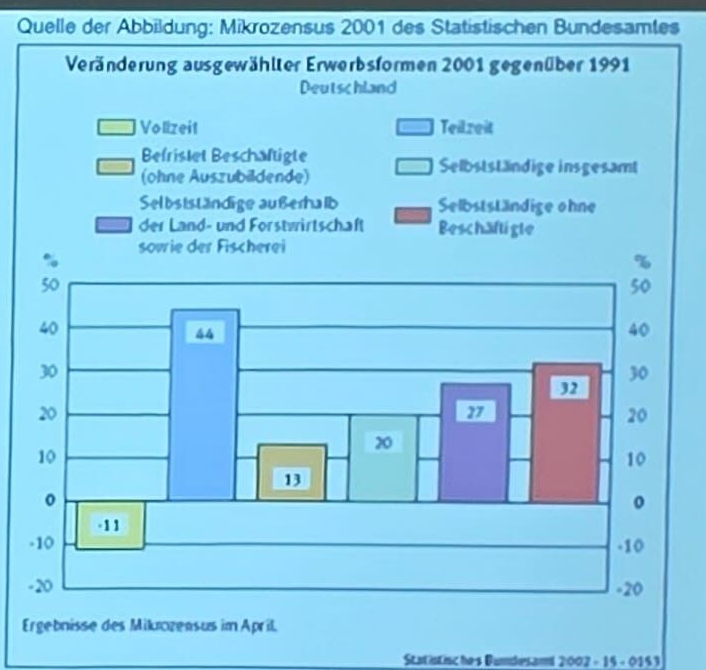
\includegraphics[width=0.8\textwidth]{figures/5_2.png} % Platzhalter für die Grafik
    \caption{Quelle: Statistisches Bundesamt, Mikrozensus 2001}
    \label{fig:scheinselbststaendigkeit}
\end{figure}
}
\exercise{5\textbar 3}{„Small is beautiful“}

\textbf{Aufgabe:}  
In Deutschland gibt es viele kleine und mittlere Unternehmen, die auf den Weltmärkten sehr erfolgreich sind.  
Wie kann man erklären, dass Großunternehmen nicht grundsätzlich wettbewerbsfähiger sind als kleine Unternehmen?

\solution{

\begin{itemize}
    \item Ein \textbf{großes Unternehmen} hat viele \textbf{Vorteile} gegenüber einem kleinen:
    \begin{itemize}
        \item So können die Durchschnittskosten bei einer steigenden Produktionsmenge sinken (\textit{„steigende Skalenerträge“}).
        \item Auch verfügt ein Großunternehmen oft über eine \textbf{bessere Verhandlungsposition} bei Abnehmern wie auch bei Lieferanten.
    \end{itemize}
    
    \item Der \textbf{Nachteil} eines großen Unternehmens besteht jedoch darin, dass dort die \textbf{Arbeitsteilung überwiegend nach dem Prinzip der Hierarchie} organisiert ist.
    \begin{itemize}
        \item Dabei stellt sich das Problem, dass hohe Transaktionskosten durch das \textit{„Principal-Agent“-Problem} geschaffen werden, die man auch als \textit{„Motivation Costs“} bezeichnet.
    \end{itemize}
    
    \item Das kleine Unternehmen führt sehr viele Transaktionen nach dem \textbf{Prinzip des Marktes} durch, womit solche Kosten vermieden werden können.
    
    \item Die Problematik einer zu weitgehenden Unternehmenskonzentration wurde besonders deutlich in den Ländern Osteuropas und der ehemaligen Sowjetunion, in denen die Wirtschaft bis 1990 nach dem Prinzip eines einzigen Großunternehmens organisiert war.
\end{itemize}
}


\exercise{6\textbar 1}{Gleichgewicht am Markt für Speiseeis}

\textbf{Aufgabe:}  
Stellen Sie sich vor, dass in einer kleinen deutschen Stadt ein harter Konkurrenzkampf auf dem Markt für italienisches Speiseeis tobt.  

\begin{enumerate}[label=\alph*)]
    \item Das Angebot der zahlreichen Eisdielen ist beschrieben durch folgende Funktion: $p^a(x) = 2 + 0,1x$.
    \item Die Nachfrage, die vor allem durch die Studierenden der Stadt entfaltet wird, ist gegeben durch: $p^n(x) = 12 - 0,1x$.
\end{enumerate}

Da Sie selbst häufig Eisdielen besuchen, haben Sie sich vorgenommen, diesen Markt einmal etwas genauer unter die Lupe zu nehmen:

\begin{enumerate}[label=\alph*)]
    \item Berechnen Sie nun zunächst den markträumenden Preis sowie die gleichgewichtige Menge für italienisches Speiseeis.
    \item Wie hoch sind die Produzentenrente und die Konsumentenrente? Skizzieren Sie die Lösung!
\end{enumerate}

\solution{

\begin{enumerate}[label=\alph*)]
    \item \textbf{Markträumender Preis und gleichgewichtige Menge:}
    \begin{itemize}
        \item Im Marktgleichgewicht muss gelten, dass das aggregierte Angebot der aggregierten Nachfrage entspricht:
        \[
        p^a(x) = p^n(x)
        \]
        \item Setzen der Funktionen:
        \[
        2 + 0,1x = 12 - 0,1x
        \]
        \item Auflösen nach $x$:
        \[
        0,2x = 10 \implies x = 50
        \]
        (Das ist die \textbf{gleichgewichtige Menge}!)
        \item Der \textbf{markträumende Preis} kann auf zwei Arten berechnet werden:
        \[
        p^a(50) = 2 + 0,1 \cdot 50 = 7
        \]
        oder
        \[
        p^n(50) = 12 - 0,1 \cdot 50 = 7
        \]
    \end{itemize}
    \item \textbf{Konsumentenrente und Produzentenrente:}
    \begin{itemize}
        \item Konsumentenrente:
        \[
        \text{Konsumentenrente} = (12 - 7) \cdot 50 \cdot 0,5 = 125 \, \text{€}
        \]
        \item Produzentenrente:
        \[
        \text{Produzentenrente} = (7 - 2) \cdot 50 \cdot 0,5 = 125 \, \text{€}
        \]
    \end{itemize}
\end{enumerate}

\begin{figure}[H]
    \centering
    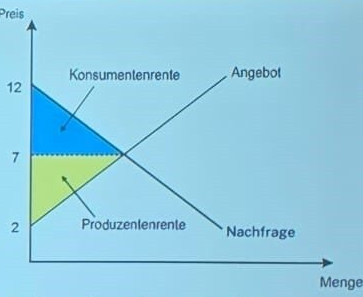
\includegraphics[width=0.5\textwidth]{figures/6_1.png}
    \caption{Marktgleichgewicht von Angebot und Nachfrage für Speiseeis}
    \label{fig:ice_market}
\end{figure}
}
\exercise{6\textbar 2}{Schocks am Markt für Speiseeis}

\textbf{Aufgabe:}  
In diesem Jahr haben zahlreiche Ereignisse Einfluss auf den Markt für italienisches Speiseeis genommen:

\begin{itemize}
    \item Eine neue Fachhochschule wird eröffnet.
    \item Der Preis für Langnese-Eis sinkt.
    \item Der Stundenlohn für Eisverkäufer steigt aufgrund gestiegener Krankenkassenbeiträge.
    \item Die Hygieneanforderungen werden verschärft.
    \item Die BAföG-Sätze werden gesenkt.
\end{itemize}

Skizzieren Sie jeweils die Effekte, die hiervon auf die Angebots- und Nachfragekurve ausgehen!

\solution{

Die Lösung visualisiert die Auswirkungen auf Angebots- und Nachfragekurven in den gegebenen Szenarien. Die entsprechenden Diagramme sind in Abbildung \ref{fig:ice_market_shocks} dargestellt.

\begin{figure}[H]
    \centering
    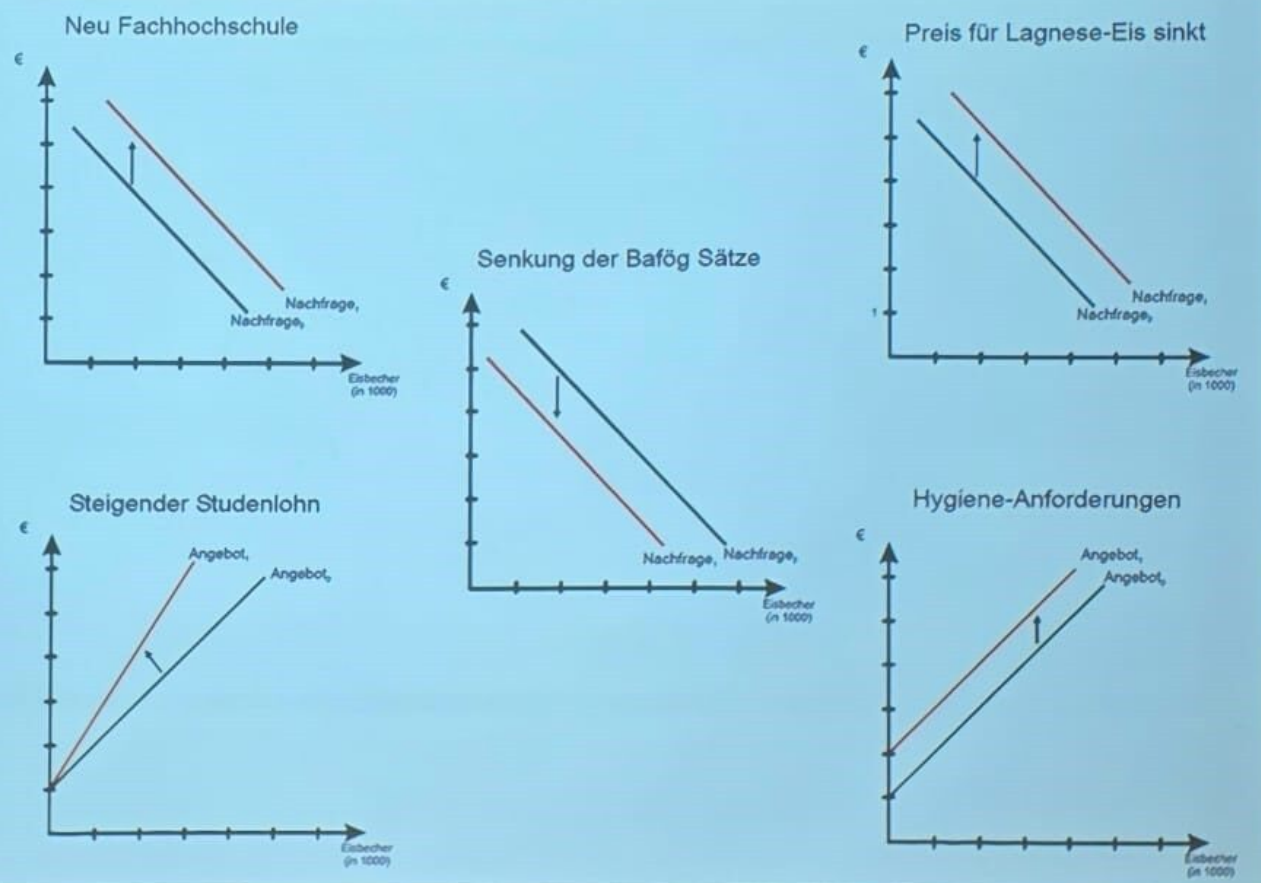
\includegraphics[width=0.8\textwidth]{figures/6_2.png}
    \caption{Einfluss verschiedener Schocks auf den Markt für Speiseeis}
    \label{fig:ice_market_shocks}
\end{figure}
}


\exercise{7\textbar 1}{Wettbewerbspolitik}

\textbf{Aufgabe:}

\begin{enumerate}[label=(\alph*)]
    \item Welche Motive haben Unternehmen, wettbewerbsbeschränkende Maßnahmen zu verfolgen?
    \item Wie wahrscheinlich ist es, dass es zu Kartellabsprachen unter den Unternehmen kommt?
    \item Was unterscheidet eine horizontale von einer vertikalen Fusion?
    \item Was versteht man unter einer „marktbeherrschenden Stellung“?
    \item Unter welchen Voraussetzungen sind in Europa staatliche Subventionen an Unternehmen erlaubt, sodass diese nicht unter das Beihilfeverbot fallen?
\end{enumerate}

\solution{
\begin{enumerate}[label=(\alph*)]
    \item \textbf{Motive für wettbewerbsbeschränkende Maßnahmen:}
    \begin{itemize}
        \item Reduktion des Konkurrenzdrucks und Vermeidung von Unsicherheiten.
        \item Sicherung höherer Gewinne durch mehr Marktmacht und höhere Markteintrittsbarrieren.
        \item Realisierung von Kosteneinsparungen (Economies of Scale) und Synergieeffekten.
        \item Erreichen einer dominierenden Marktposition oder Abschreckung potenzieller Konkurrenten.
        \item Persönliche Vorteile der Unternehmensführung wie Einkommenssteigerungen oder Prestigegewinne.
    \end{itemize}

    \item \textbf{Wahrscheinlichkeit von Kartellabsprachen:}
    \begin{itemize}
        \item Höhere Wahrscheinlichkeit bei:
        \begin{itemize}
            \item Wenigen Anbietern auf dem Markt.
            \item Hohen Markteintrittsbarrieren.
            \item Homogenen Gütern.
            \item Unelastischer Nachfrage.
        \end{itemize}
        \item Kartelle dienen der Reduktion der Wettbewerbsintensität und langfristigen Planbarkeit (z. B. Mitarbeiter, Investitionen).
    \end{itemize}

    \item \textbf{Unterschied zwischen horizontaler und vertikaler Fusion:}
    \begin{itemize}
        \item \textbf{Horizontale Fusion:}
        \begin{itemize}
            \item Zusammenschluss von Unternehmen derselben Branche und Produktions- oder Handelsstufe.
        \end{itemize}
        \item \textbf{Vertikale Fusion:}
        \begin{itemize}
            \item Zusammenschluss von Unternehmen entlang vor- oder nachgelagerter Wertschöpfungsstufen.
            \item Übernahme von Zulieferern oder Abnehmern.
        \end{itemize}
    \end{itemize}

    \item \textbf{Definition einer marktbeherrschenden Stellung:}
    \begin{itemize}
        \item Ein Unternehmen ist marktbeherrschend, wenn es die Fähigkeit besitzt, Preise, Produktionsmengen oder Marktbedingungen ohne wirksamen Wettbewerb zu beeinflussen.
        \item Dies schließt die Beherrschung eines wesentlichen Teils des Marktes ein.
    \end{itemize}

    \item \textbf{Voraussetzungen für staatliche Subventionen in Europa:}
    \begin{itemize}
        \item Staatliche Beihilfen sind grundsätzlich nach Art. 107 Abs. 1 AEUV verboten, wenn sie den Wettbewerb im Binnenmarkt verfälschen oder zu verfälschen drohen.
        \item Ausnahmen sind möglich, wenn Subventionen:
        \begin{itemize}
            \item Zur Förderung benachteiligter Regionen dienen.
            \item Forschung und Entwicklung unterstützen.
            \item Den Umweltschutz verbessern.
            \item Kleine und mittlere Unternehmen fördern.
            \item Ausbildungsprogramme oder Arbeitsplätze für Arbeitslose schaffen.
        \end{itemize}
        \item Beispiel: Die EU-Kommission verpflichtete Irland, 13 Mrd. Euro an illegal gewährte Steuervergünstigungen von Apple zurückzufordern.
    \end{itemize}
\end{enumerate}
}
\exercise{7\textbar 2}{Marktversagen versus Staatsversagen}
\begin{itemize}
    \item \textbf{Fragestellung:} Was versteht man unter Staatsversagen und was könnten die Gründe dafür sein?
\end{itemize}

\solution{
\textbf{Marktversagen versus Staatsversagen}
\begin{itemize}
    \item Auch wenn Marktversagen vorliegt, ist dies keine hinreichende Bedingung für staatliche Eingriffe.
    \item Es besteht die Möglichkeit, dass der Staat bzw. die staatliche Politik versagt.
    \item Marktversagen muss gegenüber dem Staatsversagen abgewogen werden, bevor gehandelt wird.
    \item \textbf{Definition:}
        \begin{itemize}
            \item Staatsversagen liegt vor, wenn staatliche Eingriffe ins Marktgeschehen zu neuen Problemen führen oder selbst mit Mängeln behaftete Marktlösungen verursachen.
        \end{itemize}
    \item \textbf{Beispiele für Staatsversagen:}
        \begin{itemize}
            \item Geregelte Marktzugangsbeschränkungen und Verzerrungen des Wettbewerbs durch Subventionen für bestimmte Marktteilnehmer.
            \item Sozialwohnungen, bei denen marktwirtschaftlich bessere Lösungen ignoriert werden.
        \end{itemize}
    \item Ineffizienzen bzw. Wohlstandsverluste durch staatliche Aktivitäten haben unterschiedliche Ursachen.
    \item Häufig sind politische Entscheidungsträger nicht in der Lage, die Präferenzen der Bürger ausreichend zu ermitteln.
    \item \textbf{Weitere Gründe:}
        \begin{itemize}
            \item Staatliche Leistungen werden zu „unentgeltlich“ oder zu nicht kostendeckenden Preisen angeboten.
            \item Unvollständige Informationen der Politiker eröffnen Interessengruppen überproportionalen Einfluss.
            \item Politiker handeln oft im Sinne von Wiederwahlwahrscheinlichkeit, Macht und Prestige.
            \item Konjunkturelle Schwankungen können durch staatliches Verhalten verstärkt werden.
        \end{itemize}
\end{itemize}
}

\exercise{7\textbar 3}{Höchstpreise}
\begin{enumerate}[label=(\alph*)]
    \item Wozu dienen Höchstpreise?
    \item Was passiert, wenn ein Höchstpreis über dem Marktpreis festgelegt wird?
    \item Wer bestimmt die gehandelte Menge bei einem festgelegten Höchstpreis?
    \item Welche Konsequenzen ergeben sich bei einem Nachfrageüberhang bei Festlegung eines Höchstpreises?
    \item Warum kann sich die Situation auf dem offiziellen Markt bei Festlegung eines Höchstpreises noch verschärfen?
    \item Welche Maßnahmen kann der Staat ergreifen, um die negativen Folgen einer Höchstpreisregelung zu mildern bzw. zu verhindern?
\end{enumerate}

\solution{
\begin{enumerate}[label=(\alph*)]
    \item \textbf{Wozu dienen Höchstpreise?}\\
    Höchstpreise sollen die Nachfrager besserstellen als bei freier Marktpreisbildung. Sie werden deshalb vor allem für lebensnotwendige Güter (z. B. Brot oder Wohnungsmieten) seitens des Staates angeordnet.

    \item \textbf{Was passiert, wenn ein Höchstpreis über dem Marktpreis festgelegt wird?}\\
    In diesem Fall kommt der Marktpreis zur Anwendung. Damit Höchstpreise ihre gewünschte Wirkung entfalten, müssen die Höchstpreise unter dem Gleichgewichtspreis liegen.

    \item \textbf{Wer bestimmt die gehandelte Menge bei einem festgelegten Höchstpreis?}\\
    Die Anbieter des Gutes bestimmen über die von ihnen festgelegte Menge des Angebots.\\
    \textbf{Hintergrund:}
    \begin{itemize}
        \item Ein Höchstpreis, der unterhalb des Gleichgewichtspreises liegt, führt dazu, dass die nachgefragte Menge steigt, während die angebotene Menge sinkt.
        \item Der Grund liegt darin, dass bei einem niedrigeren maximalen Preis einige Unternehmen ihre Grenzkosten nicht mehr decken können und aus dem Markt austreten.
        \item Es kommt zu einem Nachfrageüberhang, sodass viele Nachfrager leer ausgehen, da sich im Marktgleichgewicht immer nur die kürzere Marktseite durchsetzt.
    \end{itemize}

    \item \textbf{Welche Konsequenzen ergeben sich bei einem Nachfrageüberhang bei Festlegung eines Höchstpreises?}\\
    Vorausgesetzt, der Staat belässt es allein bei der Festsetzung eines Höchstpreises, kommt es zu einer Reihe von negativen Wirkungen:
    \begin{itemize}
        \item Nur die Nachfrager, die am schnellsten auf dem Markt sind (Windhundverfahren), oder die geduldigsten in der Warteschlange werden bedient.
        \item Es bildet sich ein Schwarzmarkt heraus, auf dem sich der illegale Preis als Marktpreis einstellt.
    \end{itemize}

    \item \textbf{Warum kann sich die Situation auf dem offiziellen Markt bei Festlegung eines Höchstpreises noch verschärfen?}\\
    Ist der Schwarzmarkt einmal etabliert:
    \begin{itemize}
        \item Unternehmen halten mehr und mehr Güter vom offiziellen Markt zurück, um sie auf dem Schwarzmarkt zu höheren Preisen zu verkaufen.
        \item Nachfrager nutzen den offiziellen Markt nur, um Güter auf dem Schwarzmarkt gewinnbringend weiterzuverkaufen.
        \item Das Angebotsdefizit auf dem offiziellen Markt verschärft sich.
    \end{itemize}

    \item \textbf{Welche Maßnahmen kann der Staat ergreifen, um die negativen Folgen einer Höchstpreisregelung zu mildern bzw. zu verhindern?}\\
    \begin{itemize}
        \item Staatliche Maßnahmen können das Angebot ausweiten (z. B. Subventionen, Zollsenkungen, staatliche Unternehmen).
        \item Alternativ kann die Nachfrage reduziert werden (z. B. Subventionen für Substitutionsgüter).
    \end{itemize}
    \begin{figure}[H]
        \centering
        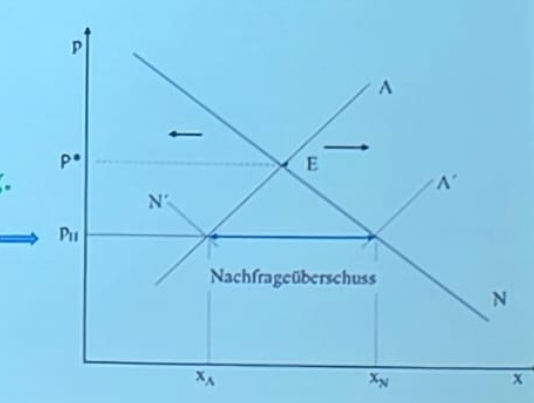
\includegraphics[width=0.4\textwidth]{figures/7_2.png}
        \caption{Marktmechanismen bei Höchstpreisen}
    \end{figure}
\end{enumerate}
}
\exercise{7\textbar 4}{Mindestpreise}
\begin{enumerate}[label=(\alph*)]
    \item Wozu dienen Mindestpreise?
    \item Muss ein Mindestpreis immer über dem Gleichgewichtspreis liegen?
\end{enumerate}

\solution{

\begin{enumerate}[label=(\alph*)]
    \item \textbf{Wozu dienen Mindestpreise?}
    \begin{itemize}
        \item Mit der Einführung von Mindestpreisen sollen die Anbieter besser gestellt werden.
        \item Die Festlegung von Mindestpreisen bedeutet, dass der Marktpreis für ein Gut eine bestimmte Höhe nicht unterschreiten, wohl aber überschreiten darf.
        \item Eingesetzt wird er hauptsächlich dort, wo den Anbietern ein bestimmtes Einkommen gesichert werden soll (z. B. in der Landwirtschaft).
    \end{itemize}

    \item \textbf{Muss ein Mindestpreis immer über dem Gleichgewichtspreis liegen?}
    \begin{itemize}
        \item Ja, der Mindestpreis muss über dem Gleichgewichtspreis liegen.
        \item Ihn darunter festzulegen, bliebe ohne praktische Auswirkung, da dann der höher liegende Marktpreis verwirklicht würde.
    \end{itemize}
\end{enumerate}
}



\end{document}

